
%%%%%%%%%%%%%%%%%%%%%%% file template.tex %%%%%%%%%%%%%%%%%%%%%%%%%
%
% This is a general template file for the LaTeX package SVJour3
% for Springer journals.          Springer Heidelberg 2010/09/16
%
% Copy it to a new file with a new name and use it as the basis
% for your article. Delete % signs as needed.
%
% This template includes a few options for different layouts and
% content for various journals. Please consult a previous issue of
% your journal as needed.
%
%%%%%%%%%%%%%%%%%%%%%%%%%%%%%%%%%%%%%%%%%%%%%%%%%%%%%%%%%%%%%%%%%%%
%
% First comes an example EPS file -- just ignore it and
% proceed on the \documentclass line
% your LaTeX will extract the file if required
\begin{filecontents*}{example.eps}
%!PS-Adobe-3.0 EPSF-3.0
%%BoundingBox: 19 19 221 221
%%CreationDate: Mon Sep 29 1997
%%Creator: programmed by hand (JK)
%%EndComments
gsave
newpath
  20 20 moveto
  20 220 lineto
  220 220 lineto
  220 20 lineto
closepath
2 setlinewidth
gsave
  .4 setgray fill
grestore
stroke
grestore
\end{filecontents*}
%
\RequirePackage{fix-cm}
%
\documentclass{svjour3}                     % onecolumn (standard format)
%\documentclass[smallcondensed]{svjour3}     % onecolumn (ditto)
%\documentclass[smallextended]{svjour3}       % onecolumn (second format)
%\documentclass[twocolumn]{svjour3}          % twocolumn
%
\smartqed  % flush right qed marks, e.g. at end of proof
%
\usepackage{graphicx}
\usepackage{caption}    
\usepackage{subfig} 
\usepackage{todonotes}
\usepackage{amsmath}
%
% \usepackage{mathptmx}      % use Times fonts if available on your TeX system
%
% insert here the call for the packages your document requires
%\usepackage{latexsym}
% etc.
%
% please place your own definitions here and don't use \def but
% \newcommand{}{}
%
% Insert the name of "your journal" with
% \journalname{myjournal}
%
\begin{document}

\title{The Pandora multi-algorithm approach to automated pattern recognition of cosmic-ray muon and test beam particle interactions in the ProtoDUNE-SP detector
%\thanks{Grants or other notes
%about the article that should go on the front page should be
%placed here. General acknowledgments should be placed at the end of the article.}
}
%\subtitle{Do you have a subtitle?\\ If so, write it here}

\author{S. Green \and
        J. Marshall \and 
        L. Escudero Sanchez \and 
        A. Blake
}

\titlerunning{The Pandora Reconstruction for ProtoDUNE-SP}
%\authorrunning{Short form of author list} % if too long for running head

\institute{S. Green \at
            University of Cambridge, Cambridge, CB3 0HE, United Kingdom
%           \emph{Present address:} of F. Author  %  if needed
            \and
            J. Marshall \at
            University of Warwick
            \and 
            L. Escudero Sanchez \at
            University of Cambridge, Cambridge, CB3 0HE, United Kingdom
            \and 
            A. Blake \at 
            University of Lancaster
}

\date{Received: date / Accepted: date}
% The correct dates will be entered by the editor

\maketitle

\begin{abstract}
Pattern recognition is an essential aspect of event reconstruction at Liquid-Argon Time-Projection Chamber detectors.  The Pandora software package has been developed and successfully applied to several ongoing neutrino LArTPC detector experiments.  Now Pandora is being applied to ProtoDUNE-SP, a test beam experiment prototyping detector technologies for use at the DUNE far detector.  The Pandora multi-algorithm approach to pattern recognition enables complex, high energy test beam particle interaction topologies to be reconstructed successfully and the interaction hierarchy determined.  This paper gives an overview of the Pandora reconstruction algorithms used for ProtoDUNE-SP and evaluates the performance for both simulation and data.
\keywords{Pattern recognition \and Event reconstruction \and Neutrino detectors \and Time-projection chambers \and DUNE \and ProtoDUNE-SP}
% \PACS{PACS code1 \and PACS code2 \and more}
% \subclass{MSC code1 \and MSC code2 \and more}
\end{abstract}

\section{Introduction}
\label{sec:intro}
ProtoDUNE-SP is a single phase liquid argon time projection chamber (LArTPC) detector prototype for the DUNE far detector.  It was completed and began taking data in late 2018, recording test beam data at CERNs Neutrino Platform from October to the start of the long shutdown in December.  The detector is continuing to take cosmic-ray muon data during the shutdown.  

The primary engineering goal of the ProtoDUNE-SP detector is to prototype the production of large scale TPCs for use at the DUNE far detector.  Alongside refinement of production procedures, ProtoDUNE-SP has several physics goals related to testing the reconstruction and performing detector calibration in a controlled environment.  Furthermore, measurements of the cross-section for various test beam particle species on a liquid argon target will be crucial for modeling neutrino interactions at the DUNE far detector.

Pandora is a software package that has been developed for event reconstruction in high energy physics and is now in use at ProtoDUNE-SP.  It consists of a framework, the Pandora Software Development Kit (SDK) \cite{pandorasdk}, and a number of different, experiment specific, content libraries containing the pattern recognition logic.  Although originally developed for event reconstruction at future linear $e^{+}e^{-}$ colliders, Pandora has been successfully applied for event reconstruction at LArTPC experiments including the MicroBooNE experiment \cite{pandorauboone}.  Pandora brings a multi-algorithm philosophy to event reconstruction, whereby algorithms are sequentially applied to build up the reconstruction from the raw inputs.  Each algorithm is designed to be simple and conservative in order to not introduce errors that would require resolving by subsequent algorithms.  Pandora now also incorporates machine learning techniques, such as Boosted Decision Trees (BDTs) and support vector machines, to drive key decisions that have to be made at certain junctions of the reconstruction. 

The Pandora reconstruction algorithms used at ProtoDUNE-SP mirror those used at MicroBooNE, which are extensively described in \cite{pandorauboone}.  Therefore, the aim of this paper is to give an overview of thsoe algorithms, highlighting specific ProtoDUNE-SP related developments, and to evaluate the performance of Pandora for both ProtoDUNE-SP simulation and data.  Section \ref{sec:protodunesp} describes the ProtoDUNE-SP detector and section \ref{sec:patrec} described the Pandora reconstruction.  Section \ref{sec:assesmentpatrec} demonstrate an assessment of the pattern performance for both ProtoDUNE-SP simulation and data.  

%-Abstract and introduction, covering Pandora background, its use across LArTPC programme, ProtoDUNE and aspects of the pattern recognition problem specific to ProtoDUNE.
%-ProtoDUNE details.
%-Pattern recognition. We?d reference the MicroBooNE algorithm description, give an executive summary of PandoraCosmic and explain how PandoraTestBeam differs from PandoraNu. In the MicroBooNE paper, we used a two-pass reconstruction, but explicitly said that this would become more sophisticated soon. This then allows us to explain the consolidated reconstruction properly, making this a major communication goal of the paper. Includes stitching, more on slicing, beam particle id.
%-Performance assessment, using MC and metrics consistent with MicroBooNE paper to assess quality of pattern recognition, understand contributions to efficiency, etc., but then moving into real data plots. Inclusion of all of the latest and greatest plots, with (ideally!) explanation of the key features.
%-Concluding comments (short).

\section{ProtoDUNE-SP}
\label{sec:protodunesp}
The ProtoDUNE-SP detector is a single phase liquid argon time projection chamber that is extensively described in \cite{pdtdr}.  Only the experiment details related to the pattern recognition side of the reconstruction are discussed in the following section.

The detector is a single-phase LArTPC with a rectangular cuboid geometry with the following dimensions: 7.4~m (horizontal), 6.0~m (vertical) and 7.0~m (longitudinal).  The ProtoDUNE-SP detector has a total volume of 0.77~kt making it the largest monolithic single phase LArTPC constructed to date.  The cryostat capacity required to accommodate that mass of argon is ~580~$ \text{m}^{3}$.  The nominal electric field in the active volume is 500~V/cm.  This is provided by the Cathode Plane Assembly (CPA), which is held at -180~kV, while the Anode Plane Assemblies (APAs) is effectively grounded due to the presence of a field cage.  The anode plane assembly houses three planes of wires, two induction, hereby referred to as \textit{u} and \textit{v}, and one collection, \textit{w}.  The pitch of \textit{u} and \textit{v} is 4.669~mm, while the pitch of the \textit{w} is 4.790~mm.  The \textit{u} and \textit{v} wire planes are aligned at $\pm35.7^{0}$ to the vertical, while the \textit{w} plane wires are vertical.  A right handed Cartesian coordinate system is used at ProtoDUNE-SP: $x$ defines the drift direction, $y$ the vertical and $z$ the remaining orthogonal direction.  The test beam for ProtoDUNE-SP is directed primarily along the positive $z$ direction.  

Each wire plane measures the drift time, relative to the beam trigger offset, of any induced or collected charge signals.  Hits are then formed from the waveforms produced from each wire by fitting the waveforms with a Gaussian.  Prior to the fitting, various detector effects are removed to reduce the background noise.  Each wire plane yields a 2D image of particle interactions in the LArTPC that forms the input to the pattern recognition.

Figure \ref{fig:inputhits} shows the event topology for a typical ProtoDUNE-SP event in each of the three wire plane views.  In general test beam particle interactions produce complex particle hierarchies involving both track and shower oriented topologies, while cosmic-ray muons produce highly track oriented topologies.  As ProtoDUNE-SP is a surface detector, the majority of the collected charge signals will originate from cosmic-ray muons.  The drift time for any hit produced from a cosmic-ray muon is ambiguous due to drift time being defined relative to the triggered beam time.

\begin{figure}
\centering
\subfloat[]{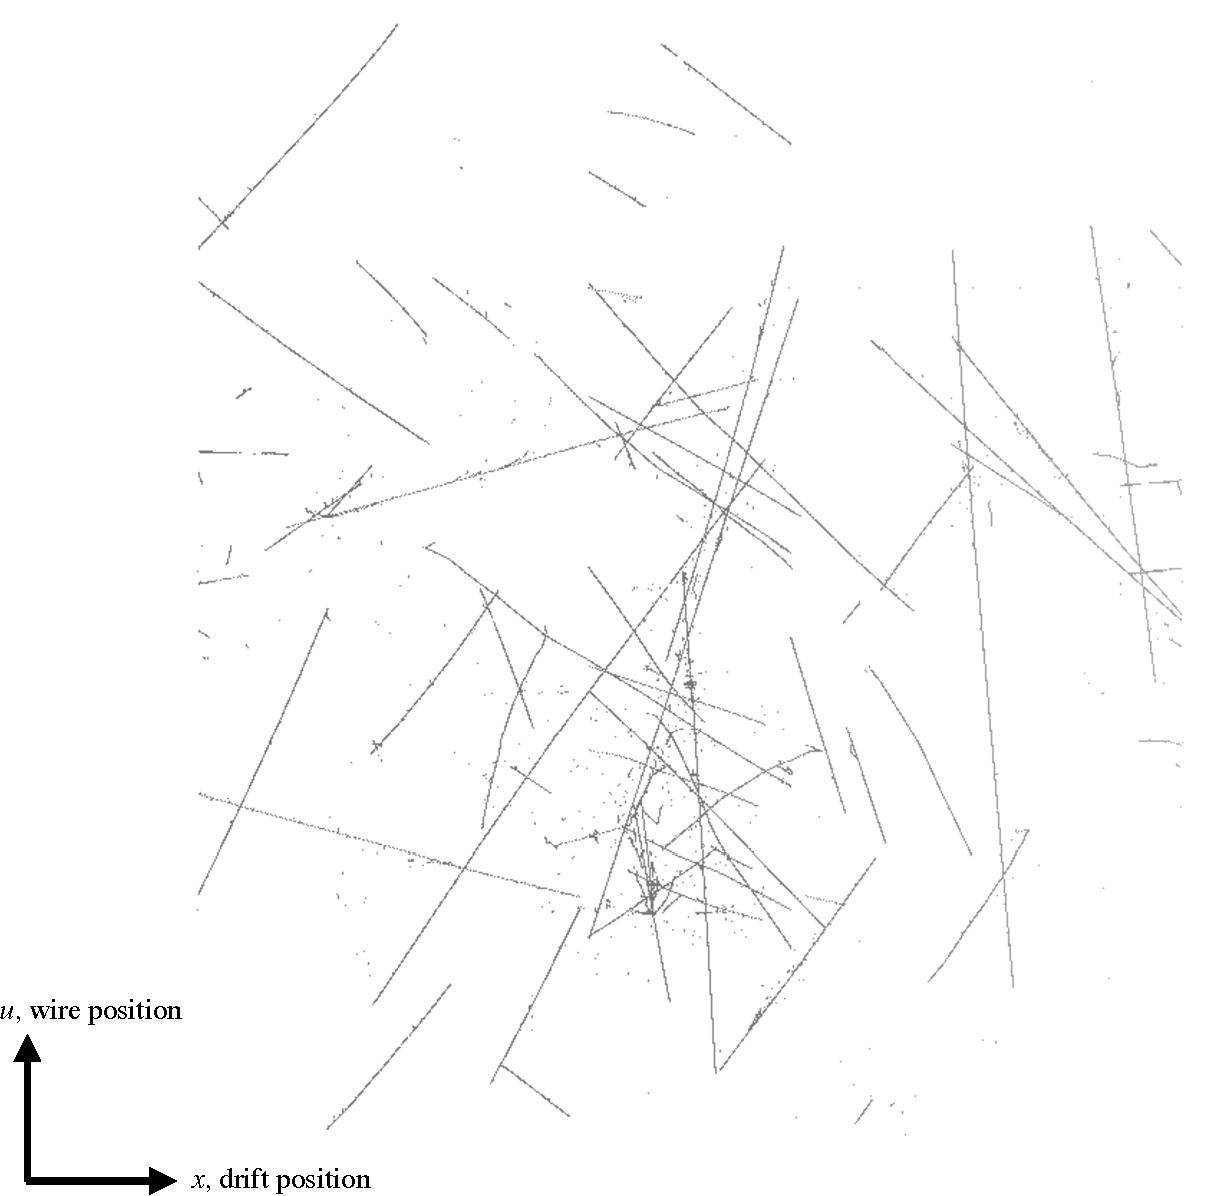
\includegraphics[width=0.3\textwidth]{Figures/EventDisplays/MC/UView.pdf}\label{fig:uview}}
\subfloat[]{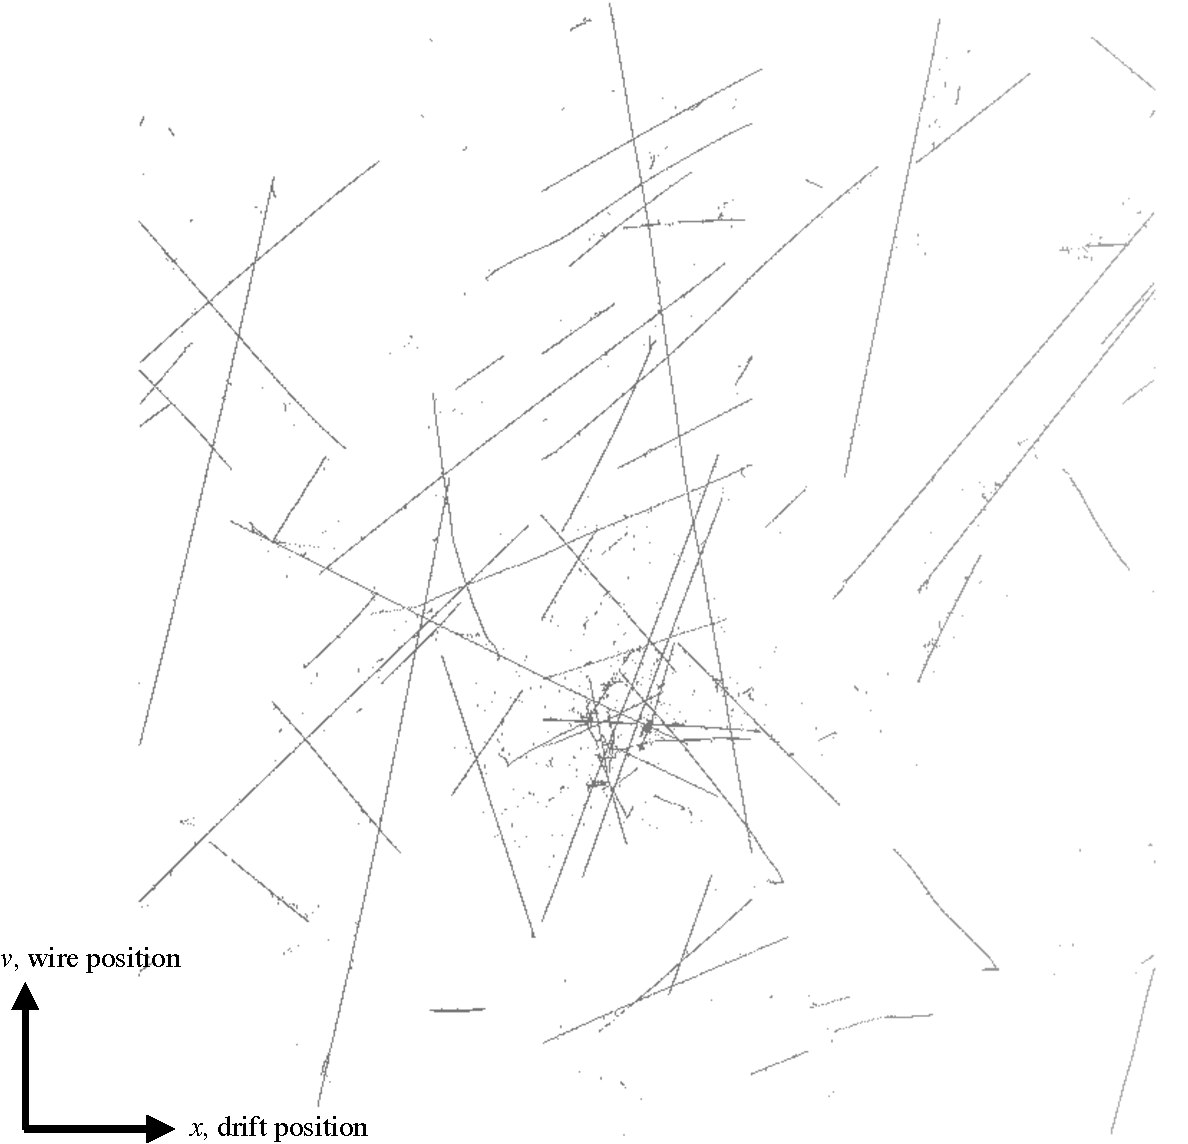
\includegraphics[width=0.3\textwidth]{Figures/EventDisplays/MC/VView.pdf}\label{fig:vview}}
\subfloat[]{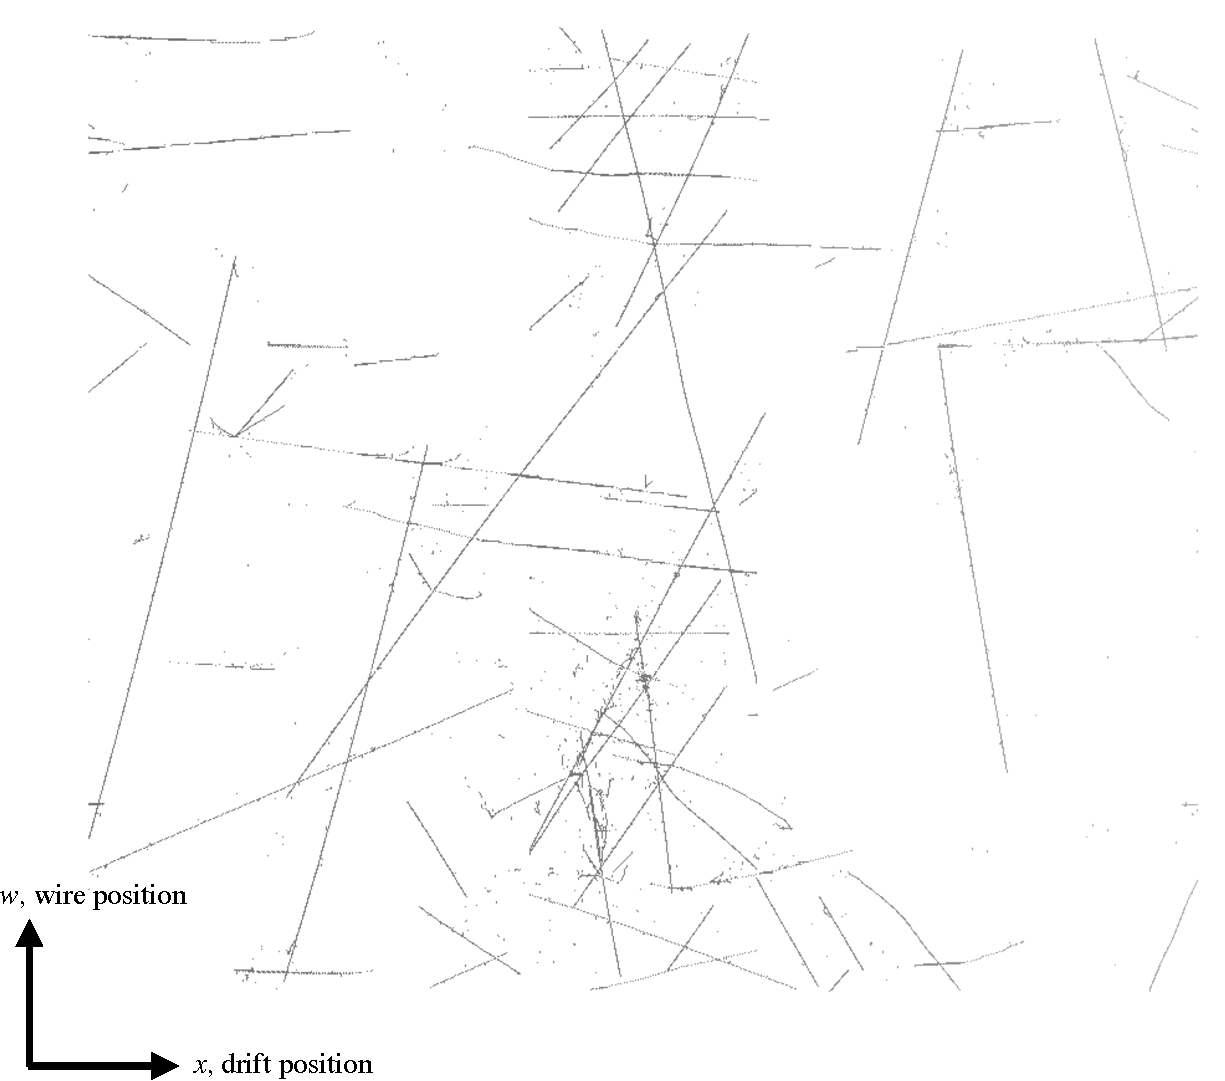
\includegraphics[width=0.3\textwidth]{Figures/EventDisplays/MC/WView.pdf}\label{fig:wview}}
\caption{The input hits on the \protect\subref{fig:uview} $u$, \protect\subref{fig:vview} $v$ and \protect\subref{fig:wview} $w$ wire planes for a simulated 5~GeV $\pi^{+}$ interaction in the ProtoDUNE-SP detector.}
\label{fig:inputhits}
\end{figure}

The CPA and APA planes in ProtoDUNE-SP contain three independent modules giving a total of twelve TPCs in the entire detector.  The outermost six TPCs have no drift field, however, particle depositing charge in these regions can still produce a signal on the wire planes.  Adjacent TPCs sharing a common drift direction are concatenated together inside Pandora to form drift volumes as illustrated in figure \ref{fig:tpcs}.  The drift direction for a given TPC is either along positive or negative $x$ depending on the local CPA and APA orientation.  Drift volumes act as effective TPCs allowing the pattern recognition to correlate inputs between adjacent TPCs trivially.

\begin{figure}
\centering
\subfloat[]{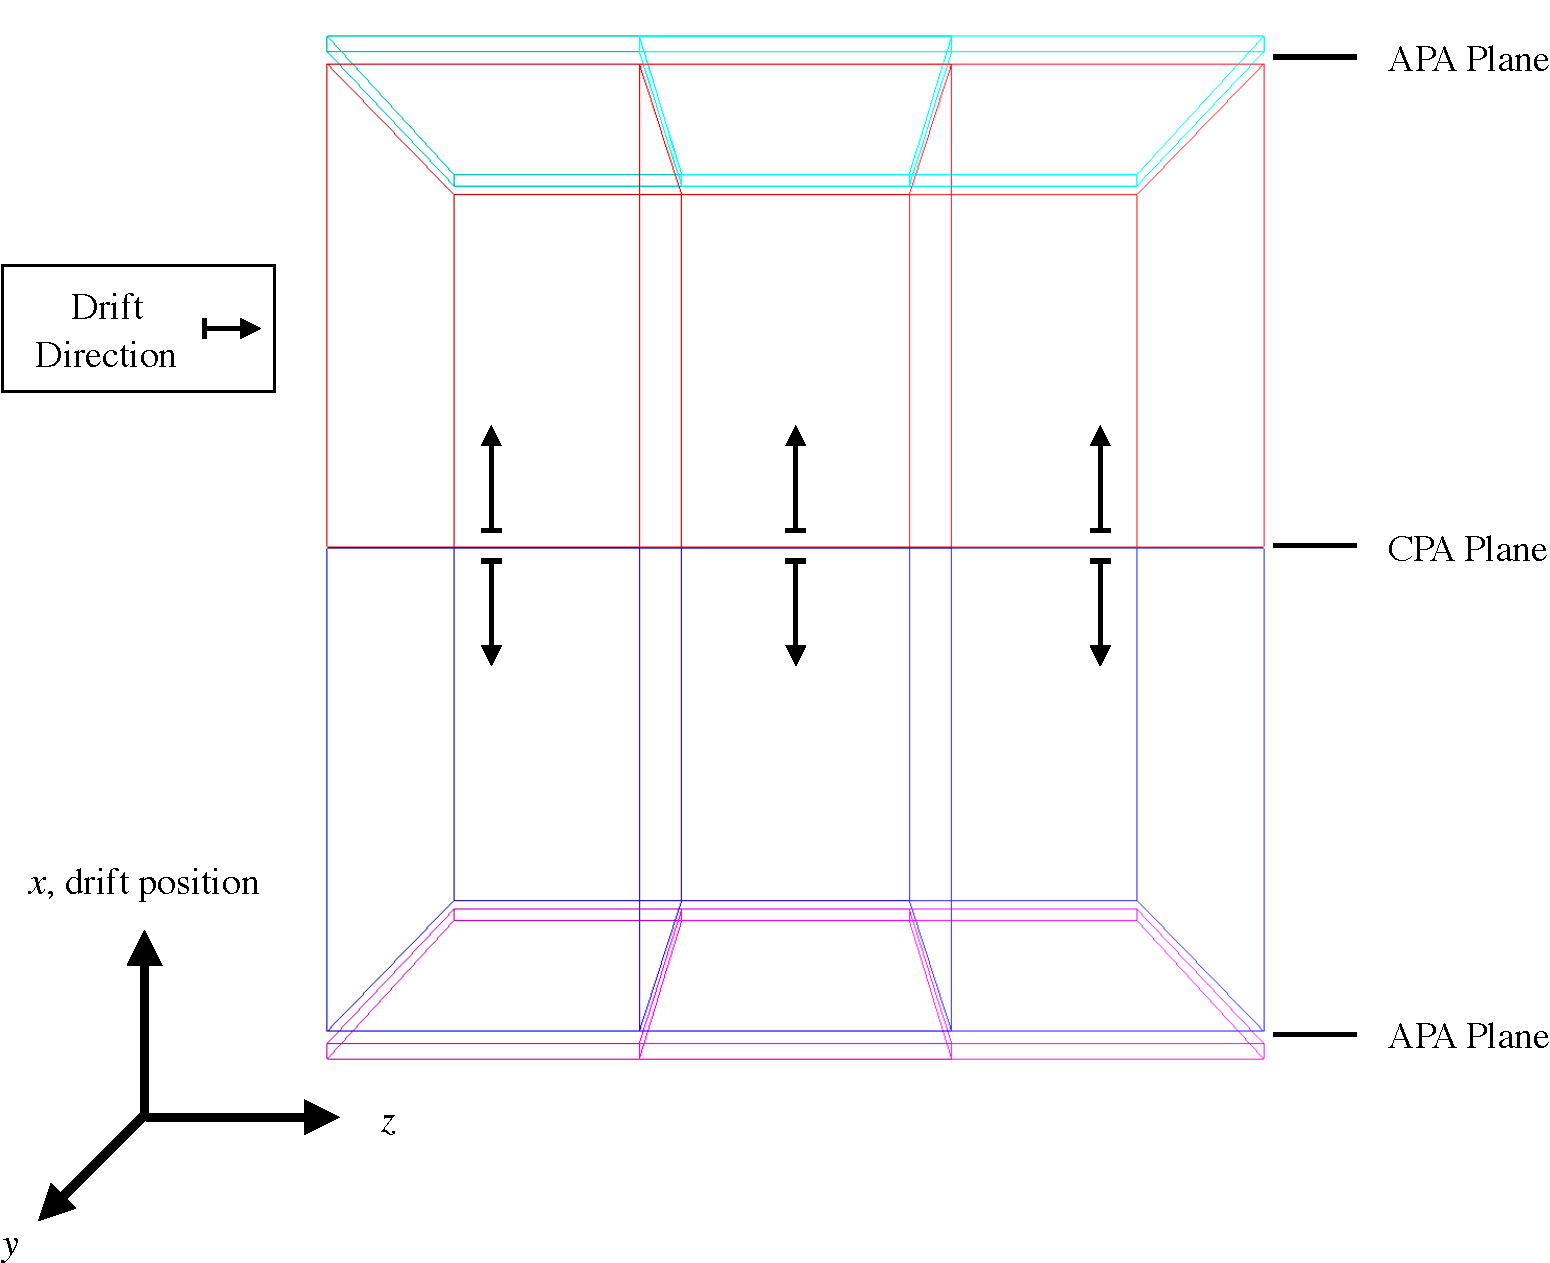
\includegraphics[width=0.5\textwidth]{Figures/Diagram/TPCs.pdf}\label{fig:tpclayout}}
\subfloat[]{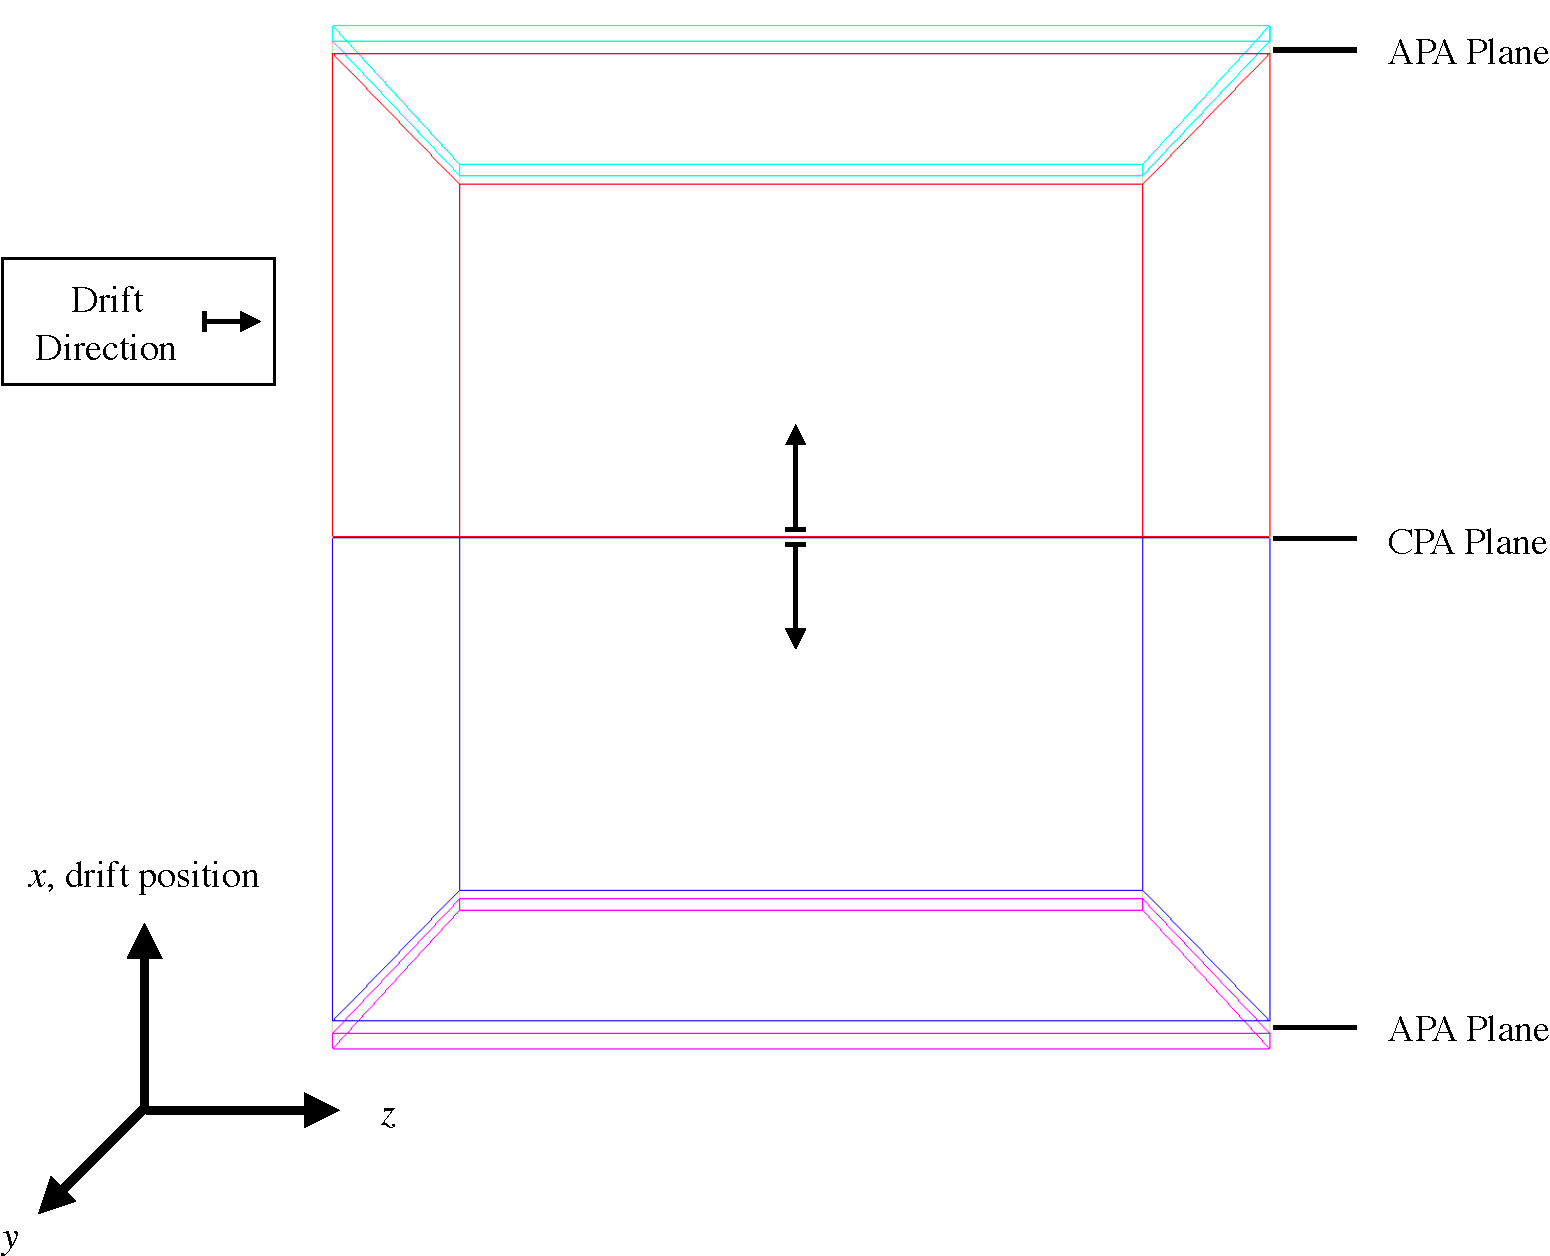
\includegraphics[width=0.5\textwidth]{Figures/Diagram/DriftVolumes.pdf}\label{fig:dvlayout}}
\caption{The layout of \protect\subref{fig:tpclayout} the twelve TPCs in ProtoDUNE-SP and \protect\subref{fig:dvlayout} the drift volumes used by Pandora.  Drift volumes are formed by concatenating adjacent TPCs with common drift direction together into a single volume.}
\label{fig:tpcs}
\end{figure}

The test beam contains a mixture of particle species; $\pi^{+}$, $e^{+}$, $\mu^{+}$, $K^{+}$ and \textit{p}.  The momentum of the beam can be varied from 0.3 to 7~GeV/c with a resolution of $\Delta p/p \leq 3\%$ \cite{pdtdr}.  The test beam enters the LArTPC through the low \textit{z} face and has a transverse beam size in the \textit{x-y} plane of $\approx$~1~cm.

A trigger system is present to identify the particle species and momentum of the test beam particle prior to the particle entering the TPC.  Beam halo particles are also present in the ProtoDUNE-SP test beam.  Beam halo are test beam particles that are produced in the creation of the beam, but that do not have the appropriate momentum to be guided to the expected location in the TPC.  These particles are not measured by the triggered but do appear in the detector surrounding the beam as illustrated in figure \ref{fig:eventdecomp}.

\begin{figure}
\centering
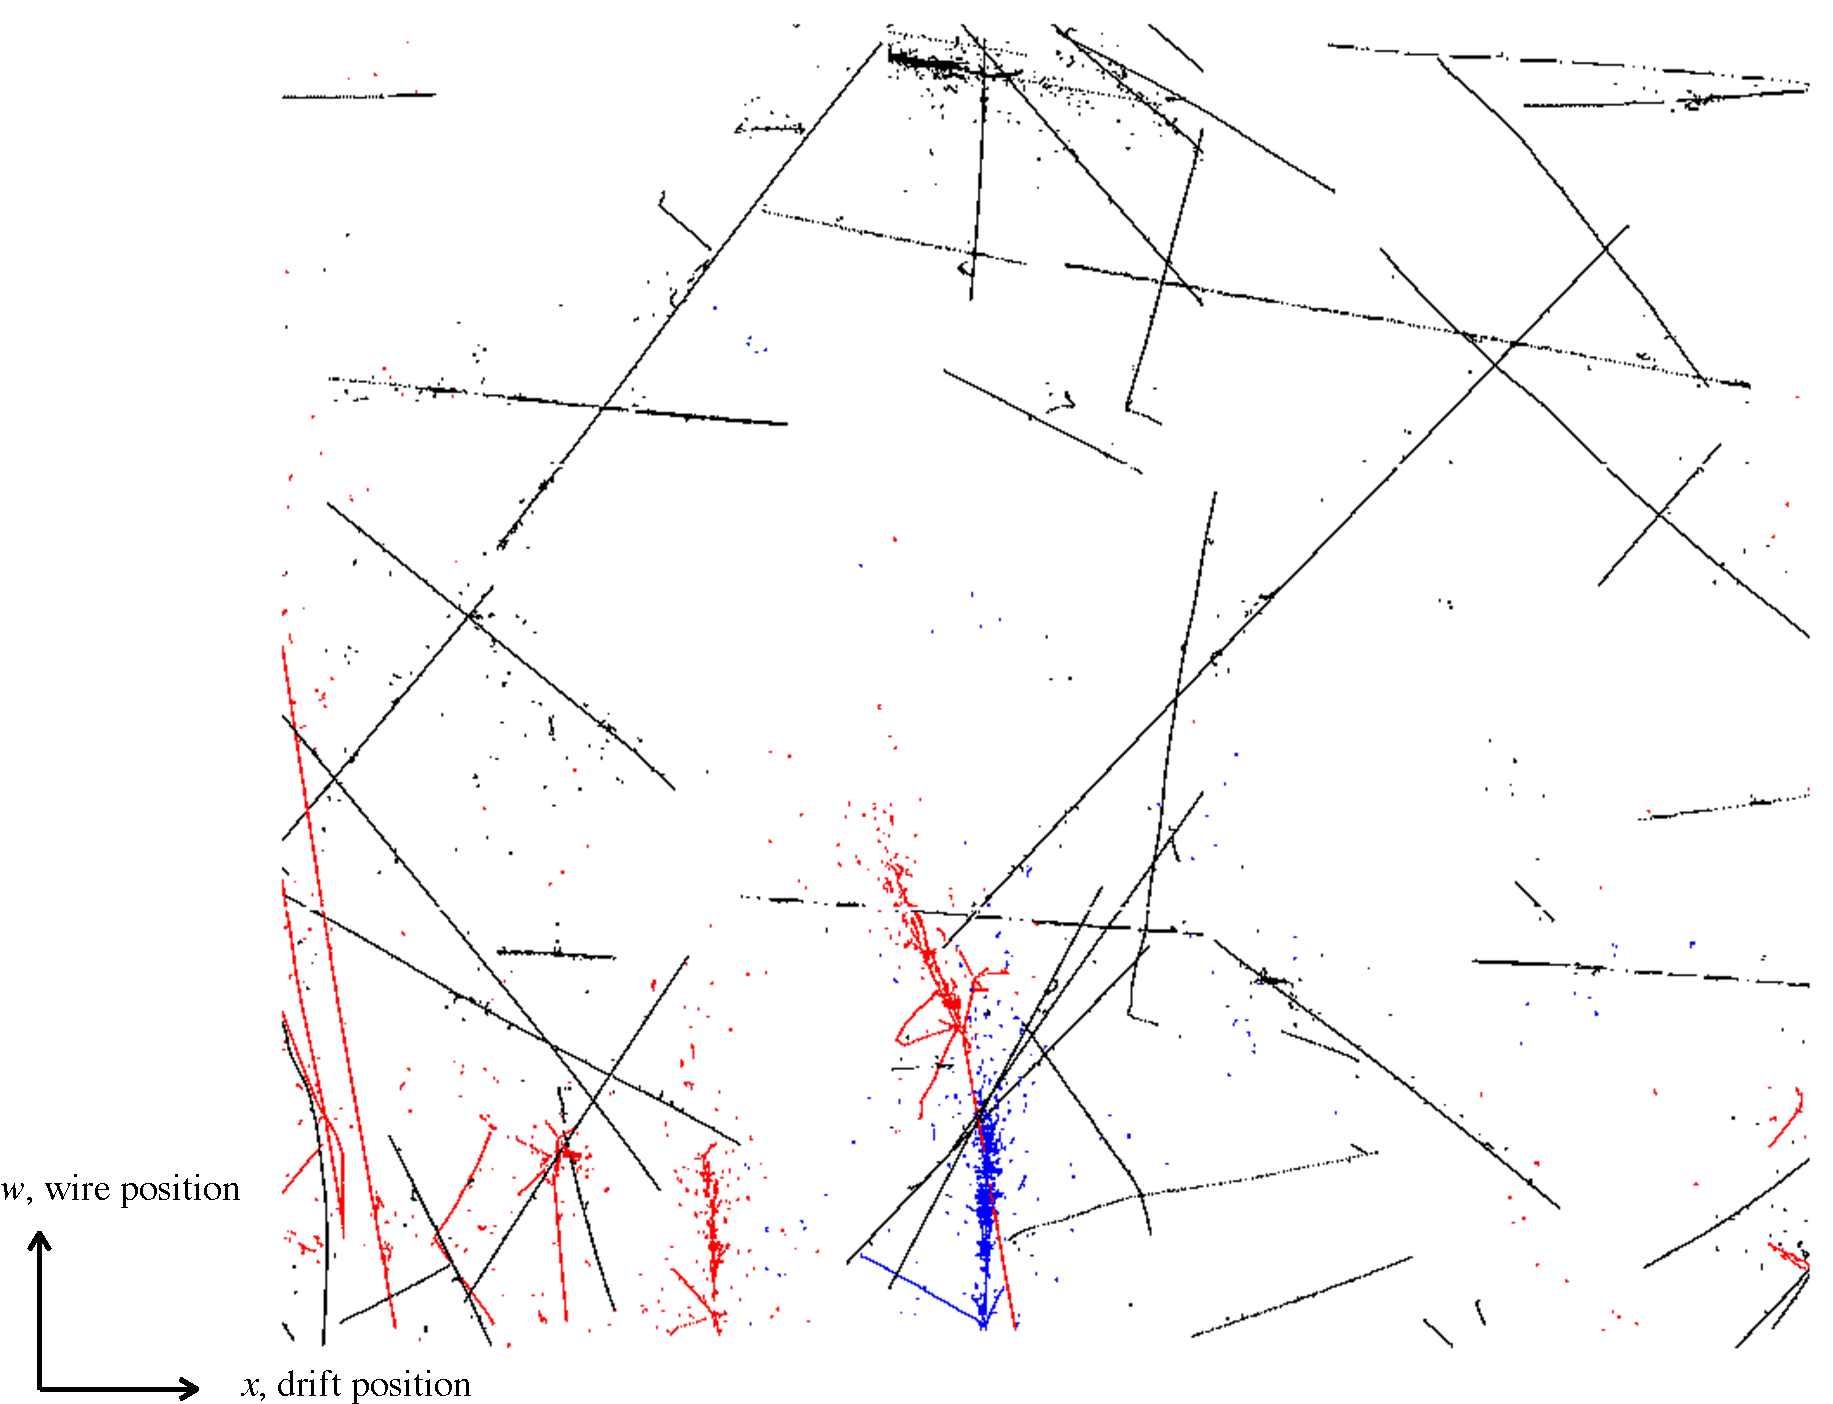
\includegraphics[width=0.5\textwidth]{Figures/EventDisplays/MC/EventComposition.pdf}
\caption{An example of the $w$ view for a simulated 7~GeV $\pi^{+}$ event at ProtoDUNE-SP where the hits have been coloured to indicate their origin; triggered beam particle (blue), beam halo (red) and cosmic-ray muon (black).}
\label{fig:eventdecomp}
\end{figure}

As ProtoDUNE-SP is a surface detector, a crucial pattern recognition goal is to distinguish the cosmic-ray muon backgrounds from the test beam particle signal.  Several other factors also affect the pattern recognition including noise filtering, fitting of the waveform and deconvolution of hit charge deposited on adjacent wires.  

\todo{Reference for noise filtering etc...}

\section{LArTPC Pattern Recognition}
\label{sec:patrec}
In order to fully exploit the imaging capabilities of LArTPCs for particle physics, a paradigm shift in the field of reconstruction is required.  The detailed images of interactions in LArTPCs make it possible to track individual charged particles throughout the detector and to build up a hierarchy describing their interactions.  This presents the reconstruction with the dual challenges of identifying and reconstructing each individual particle in an interaction and building up the hierarchy of that interaction.

The ProtoDUNE-SP LArTPC produces three sets of 2D images (wire number vs drift time) of particle interactions: the \textit{u}, \textit{v} and \textit{w} "views".  Pandora takes the approach of performing 2D reconstruction first in order to group clusters of hits together and then to correlate features of those clusters between all three views.  By correlating features across the three views, features that were obscured in certain views can be recovered.  This correlation and interpretation process is analogous to stereoscopy, whereby the brain is able to interpret the 2D inputs from the eyes into a consistent 3D world view.  It is this fundamental process that Pandora is attempting to replicate for use in LArTPC experiments.  Once consistent matches have been made across all three views, Pandora begins a 3D reconstruction phase.  The reconstruction is completed by ordering the reconstructed particles into a hierarchy. Details of the algorithm chains used in the ProtoDUNE-SP reconstruction can be found in section \ref{sec:algchains}.

\subsection{Algorithm Chains}
\label{sec:algchains}
Inside Pandora, pattern recognition logic is applied through the sequential application of individual algorithms i.e. algorithm chains.  The necessity for distinct algorithm chains relates to the underlying hypothesis that is assumed by reconstruction.  For ProtoDUNE-SP the two algorithm chains in use are Pandora Test Beam and Pandora Cosmic, which run the reconstruction assuming a test beam particle interaction and cosmic-ray muon hypothesis respectively.

The use of algorithm chains enables Pandora to take a multi-algorithm approach to pattern recognition whereby different reconstruction hypotheses are applied at any given point in the reconstruction and only the most appropriate outcome persisted.  This application of this multi-algorithm approach applied to ProtoDUNE-SP is discussed in section \ref{sec:consolidatedreco}.

\subsubsection{Pandora Test Beam}
The Pandora Test Beam algorithm chain was developed from the Pandora Neutrino algorithm chain discussed in \cite{pandorauboone}.  The philosophy of both of these algorithm chains is the identification of a primary interaction vertex, whether that be from a neutrino or a test beam particle interaction, and then reconstruct the "daughter" particles emanating from that vertex.  Once complete, an additional algorithm, the TestBeamParticleCreation algorithm, runs in the Pandora Test Beam algorithm chain to identify the primary incident test beam particle.  The reconstructed particle hierarchy is then adjusted accordingly.  An illustration showing the hierarchy before and after the implementation of this algorithm is shown in figure \ref{fig:testbeamcreation}.

\begin{figure}
\centering
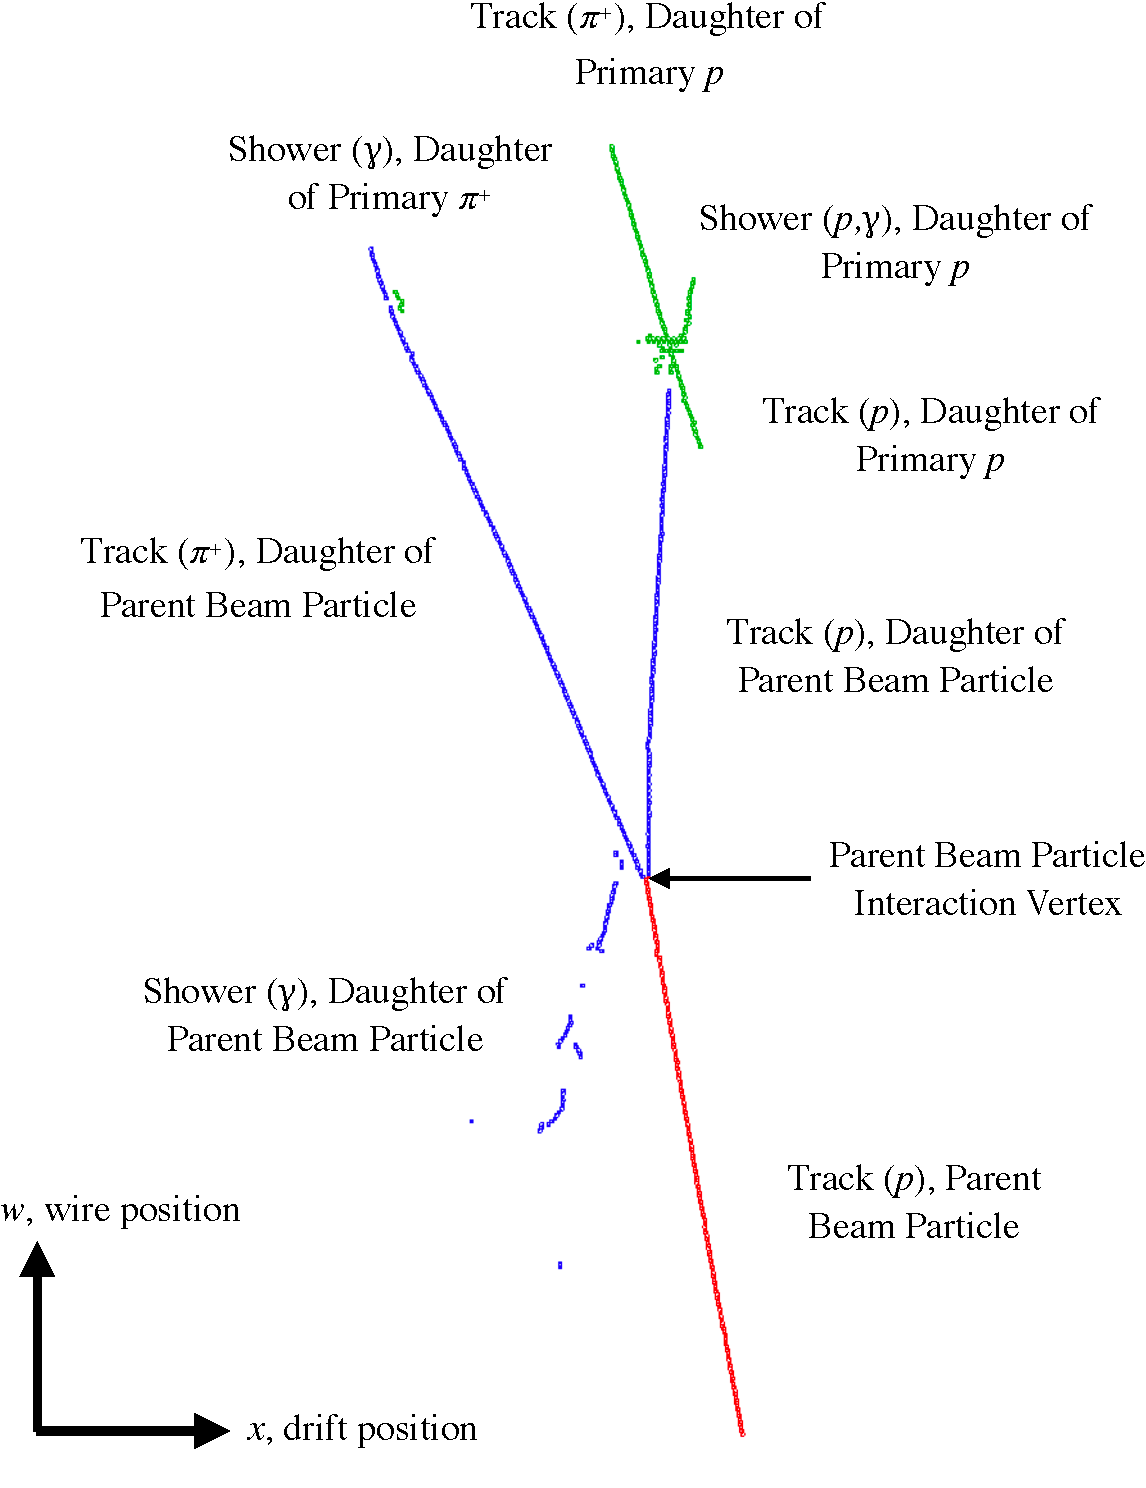
\includegraphics[width=0.5\textwidth]{Figures/EventDisplays/MC/TestBeamParticleCreation.pdf}
\caption{An example of the 2D reconstruction output for a triggered test beam particle.  The particle hierarchy has been modified by the TestBeamParticleCreation algorithm to reflect the presence of an incoming track-like parent particle.  The parent particle (red), daughters (blue) and subsequent daughters (green) have been separately highlighted.}
\label{fig:testbeamcreation}
\end{figure}

\subsubsection{Pandora Cosmic}
\label{sec:pandoracosmic}
The Pandora Cosmic algorithm chain \cite{pandorauboone} was developed to target the reconstruction of track-oriented particles i.e. cosmic-ray muons.  Reconstructed showers are assumed to be delta rays and these are added to the reconstructed hierarchy as daughter particles of the parent track-like particle.  The primary interaction vertex is taken as the highest $y$ point of the track-like parent particle.

As the ProtoDUNE-SP LArTPC detector consists of four adjacent independent drift volumes, it is possible for Pandora to identify the true time that a cosmic-ray muon passed through the detector if it crossed either the CPA or APA planes.  Any deviation from the trigger start time for the detector will result in either an increase or decrease in the effective drift time for the ionization electrons produced by the CPA or APA crossing cosmic-ray muon.  As the drift direction alternates between adjacent drift volumes in ProtoDUNE-SP, the shift in effective drift time results in two reconstructed 3D particles, one per adjacent drift volume bounding the crossed plane, being bodily shifted by equal and opposite amounts in drift position, $x$.  By associating pairs of particles in opposing drift volumes, based on the direction the particles point in and their relative locations in the y-z plane, it is possible to shift them by equal and opposite amounts in drift position until they form a consistent single 3D particle.  This process is known as "stitching" and is demonstrated in figure \ref{fig:stitching}.  The initial hit positions in the 2D view illustrates how a single cosmic-ray muon cluster, if it crosses a CPA or APA boundary and the time it enters the detector differs from the test beam trigger time, can be split up into separate clusters if the triggered test beam time is used as the offset for defining drift position.  Metrics describing the stitching precision can be found in section \ref{sec:crmetrics}.

\begin{figure}
\centering
\subfloat[]{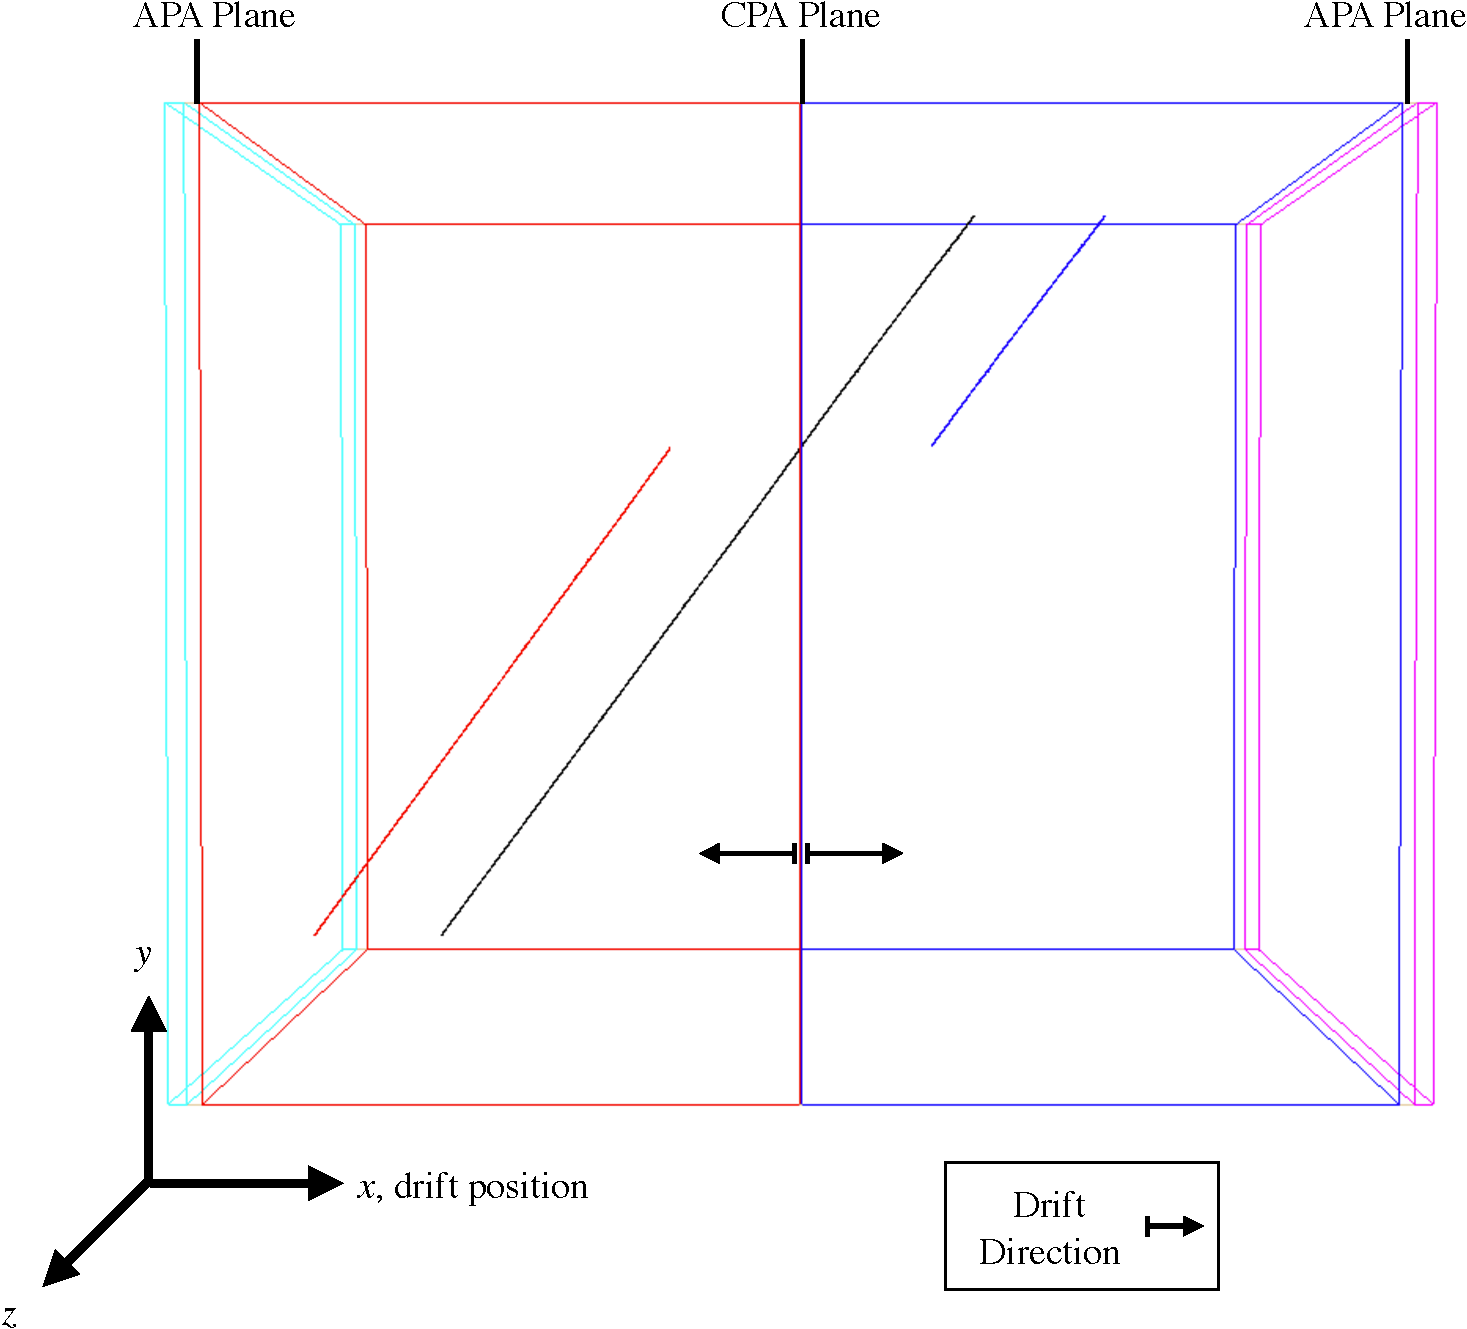
\includegraphics[width=0.5\textwidth]{Figures/EventDisplays/Stitching/Stitching.pdf}\label{fig:stitching3d}} \\
\subfloat[]{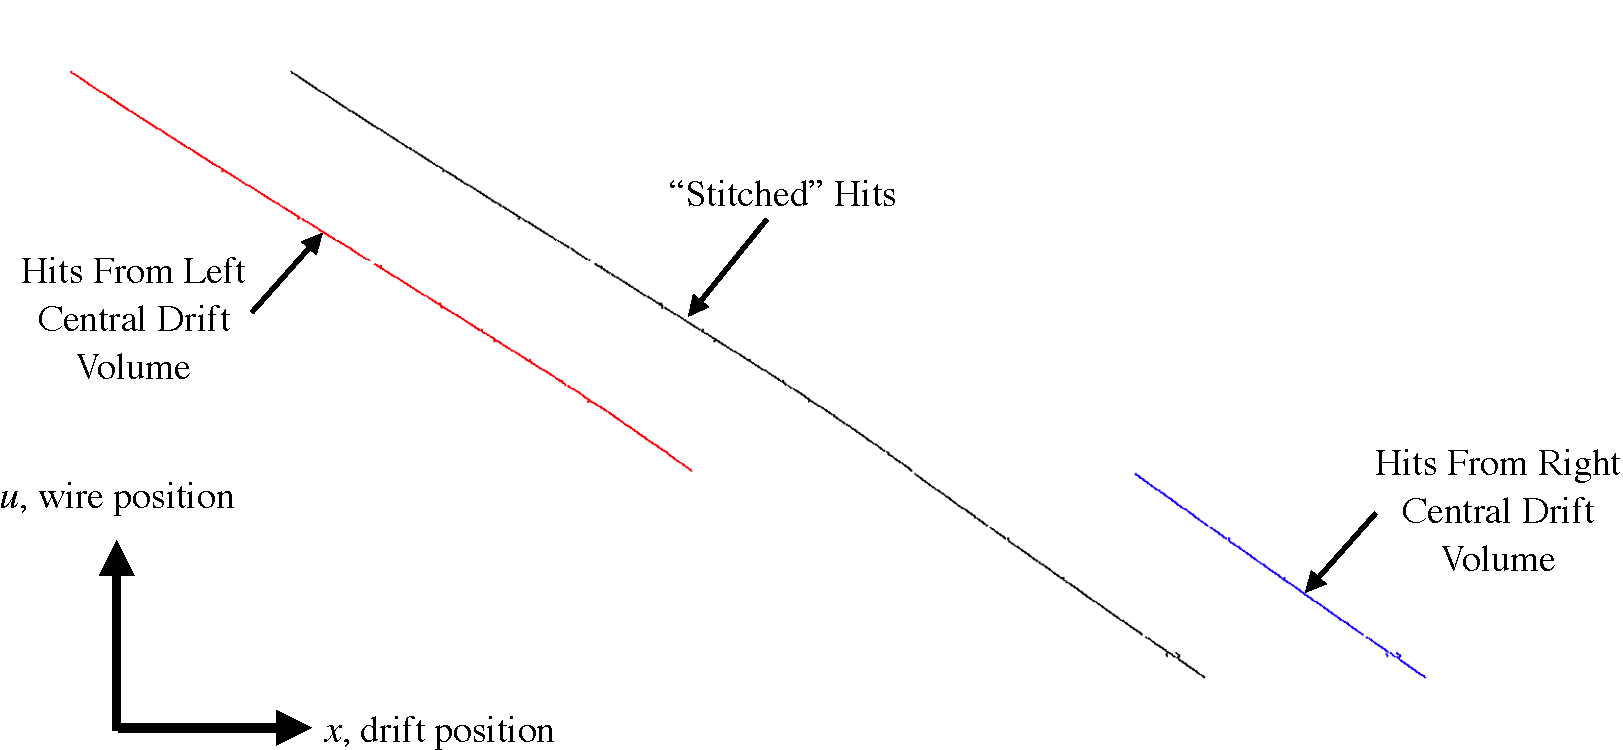
\includegraphics[width=0.5\textwidth]{Figures/EventDisplays/Stitching/Stitching_U.pdf}\label{fig:stitching2d}}
\caption{An example of the "stitching" procedure showing \protect\subref{fig:stitching3d} the 3D hits and \protect\subref{fig:stitching2d} the 2D hits from the $u$ view that were involved.  The initial two particles (red, blue) have been independently reconstructed in the two central drift volumes of ProtoDUNE-SP.  Based on pointing information and the offset in the $y$-$z$ plane, they have been identified as belonging to the same cosmic-ray muon particle.  The final stitched particle (black) is formed by applying a shift in drift position to each of the two initial particles and merging them together.}
\label{fig:stitching}
\end{figure}


\subsection{Consolidated Reconstruction}
\label{sec:consolidatedreco}
As the appropriate algorithm chain to apply to any individual parent particle interaction varies depending on whether that particle is a cosmic-ray muon or a test beam particle, additional logic beyond that contained in the algorithm chains themselves is needed to apply and persist the appropriate reconstruction. This additional logic is applied within the Pandora consolidated reconstruction, which is outlined in figure \ref{fig:consolidatedreco}.

\begin{figure}
\centering
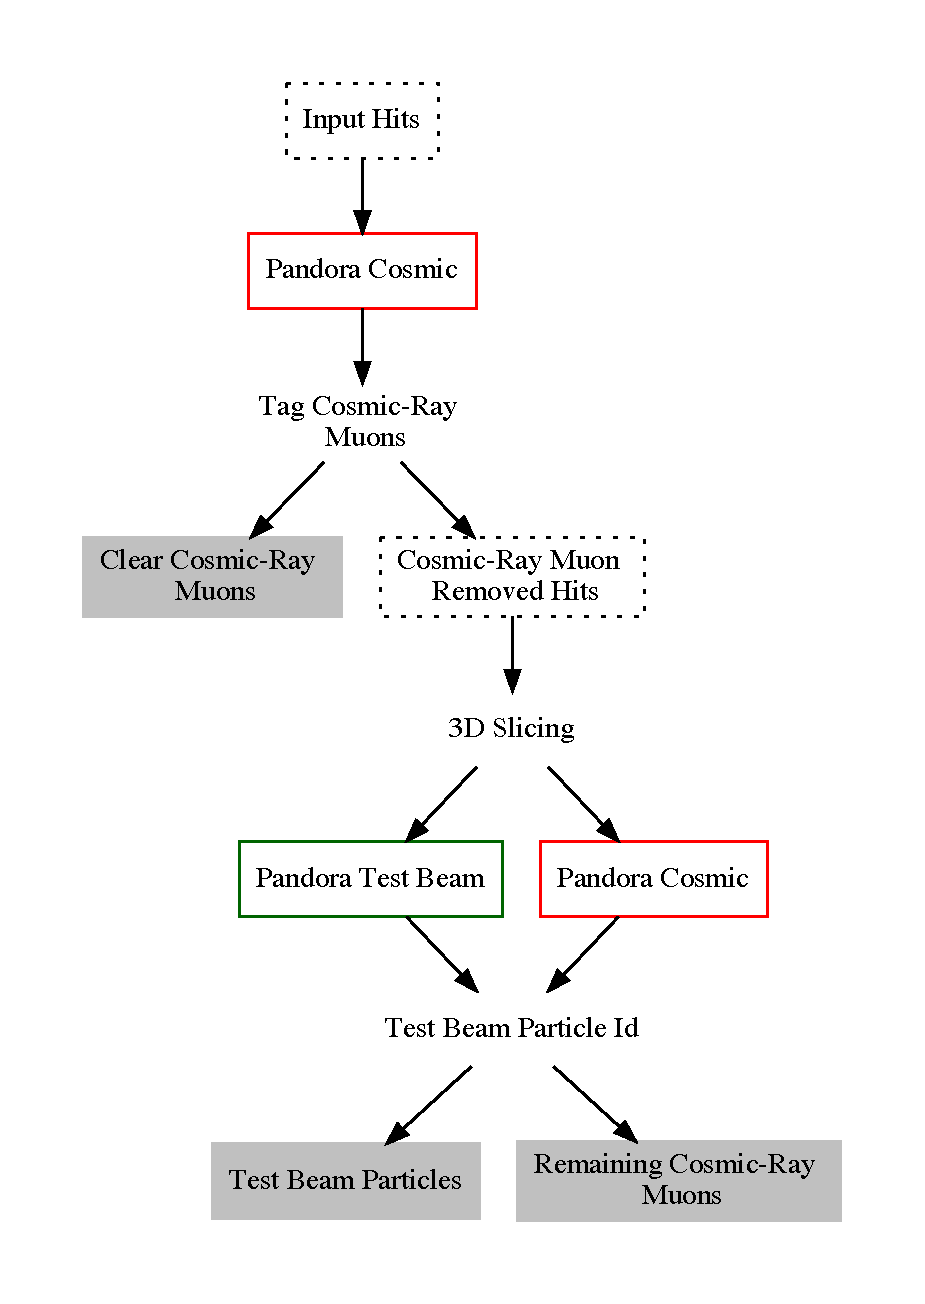
\includegraphics[width=0.75\textwidth]{Figures/Diagram/ConsolidatedReco.pdf}
\caption{Outline of the Pandora consolidated reconstruction.  Running the Pandora Test Beam and Pandora Cosmic algorithm chains on the same input hits in a given slice, a region of the detector containing hits originating from a single parent particle interaction, yields two reconstruction outputs that can be compared and the optimal reconstruction persisted.  This explicitly demonstrates the multi-algorithm approach taken by Pandora.}
\label{fig:consolidatedreco}
\end{figure}

The consolidated reconstruction begins by running the Pandora Cosmic algorithm chain that reconstructs all particles under the cosmic-ray muon particle hypothesis.  The reconstructed particles are then examined in order to determine if they are "clear" cosmic-ray muons.  The definition of a clear reconstructed cosmic-ray muon is a reconstructed particle that is highly unlikely to contain hits that originate from a test beam particle interaction.  Two distinct methods are used for identifying clear cosmic-ray muons:

\begin{itemize}
\item If the cosmic-ray muon crosses the CPA or APA plane and the reconstructed particle was stitched as described in section \ref{sec:pandoracosmic}.
\item If any hits in the reconstructed particle, assuming that the offset in the drift position for the hits is defined using the triggered test beam time, fall outside of the physical drift volume boundary as illustrated in figure \ref{fig:intime}.
\item If the reconstructed particle enters the detector through the top face and exists the lower face as illustrated in figure \ref{fig:crtopbottom}.
\end{itemize}

\begin{figure}
\centering
\subfloat[]{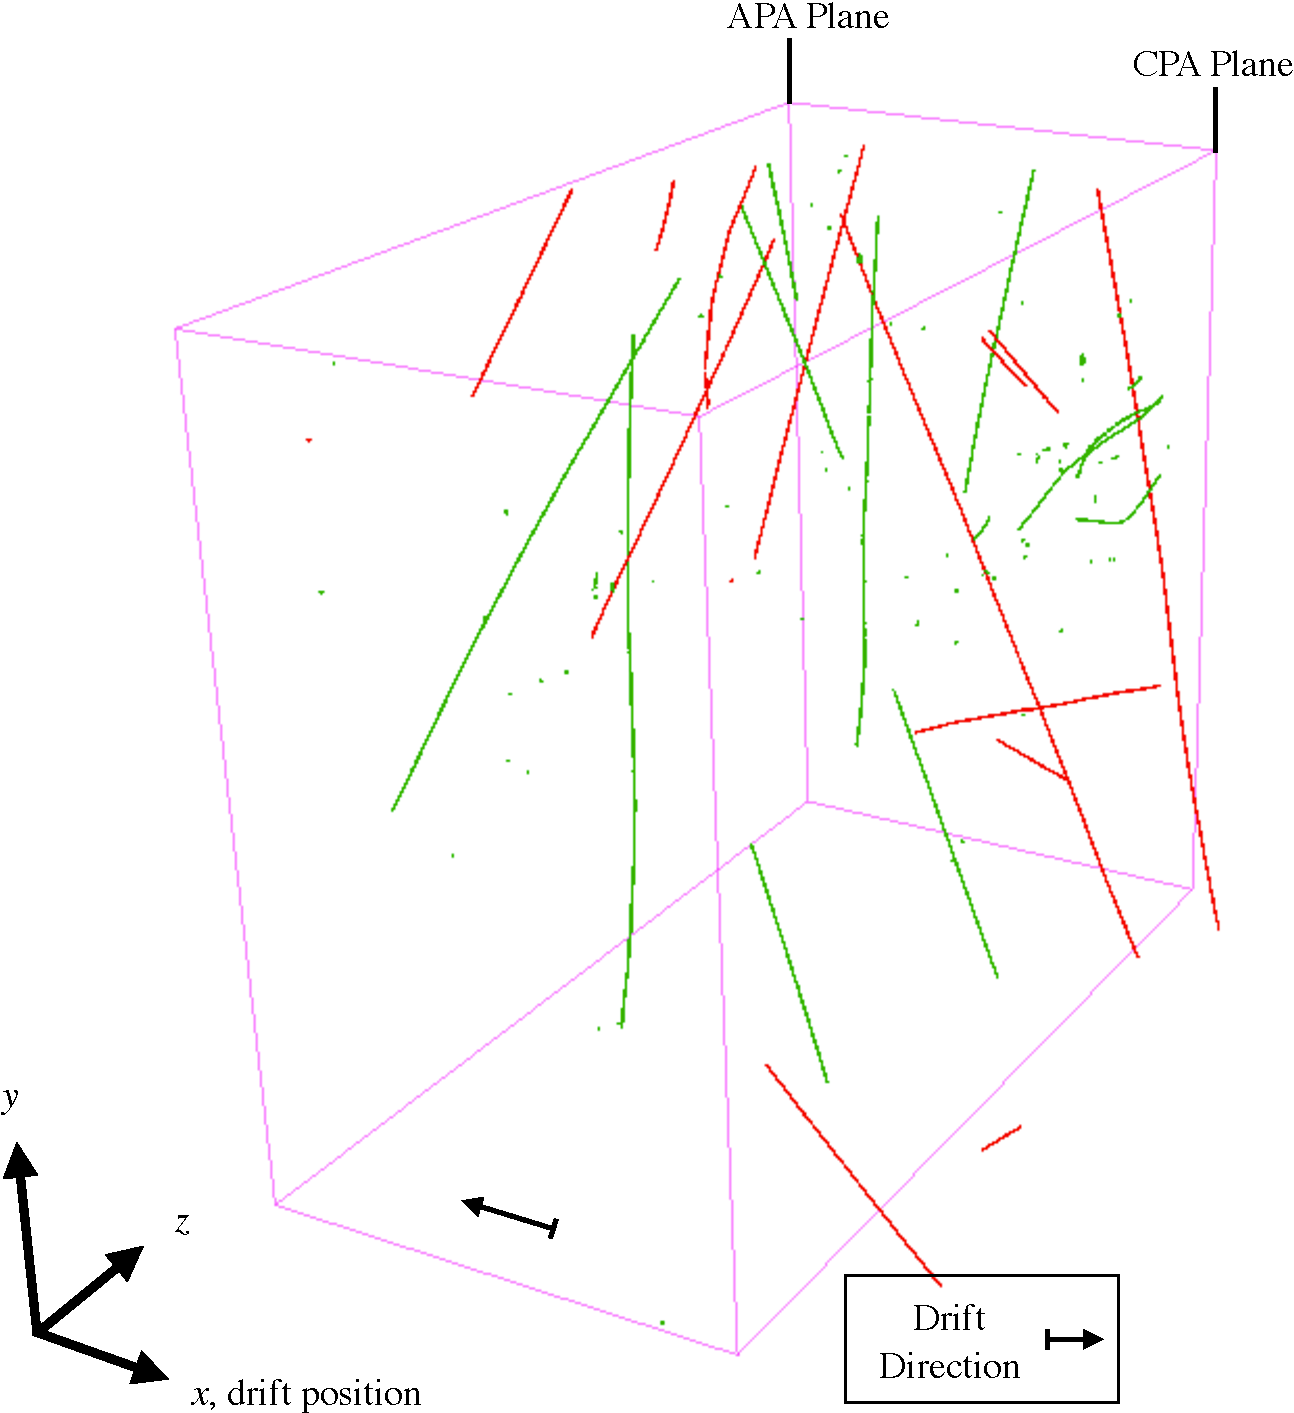
\includegraphics[width=0.3\textwidth]{Figures/Diagram/InTime/InTimeDefinition3D.pdf}\label{fig:intime3d}}
\subfloat[]{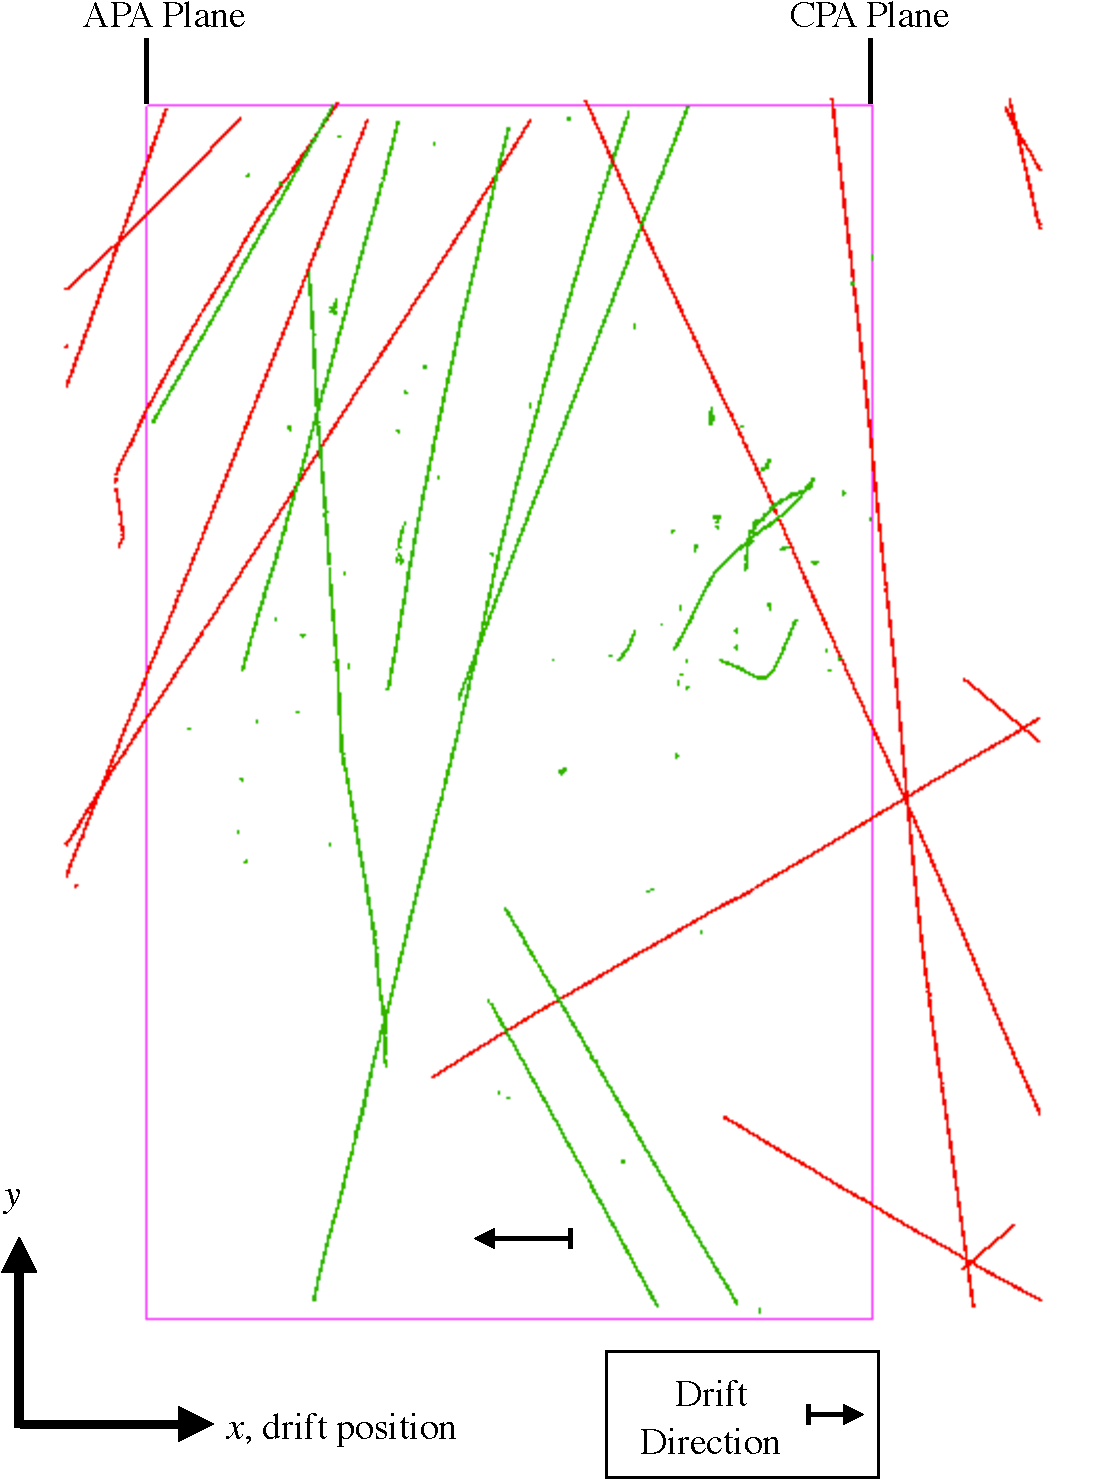
\includegraphics[width=0.3\textwidth]{Figures/Diagram/InTime/InTimeDefinitionXY.pdf}\label{fig:intimexy}}
\subfloat[]{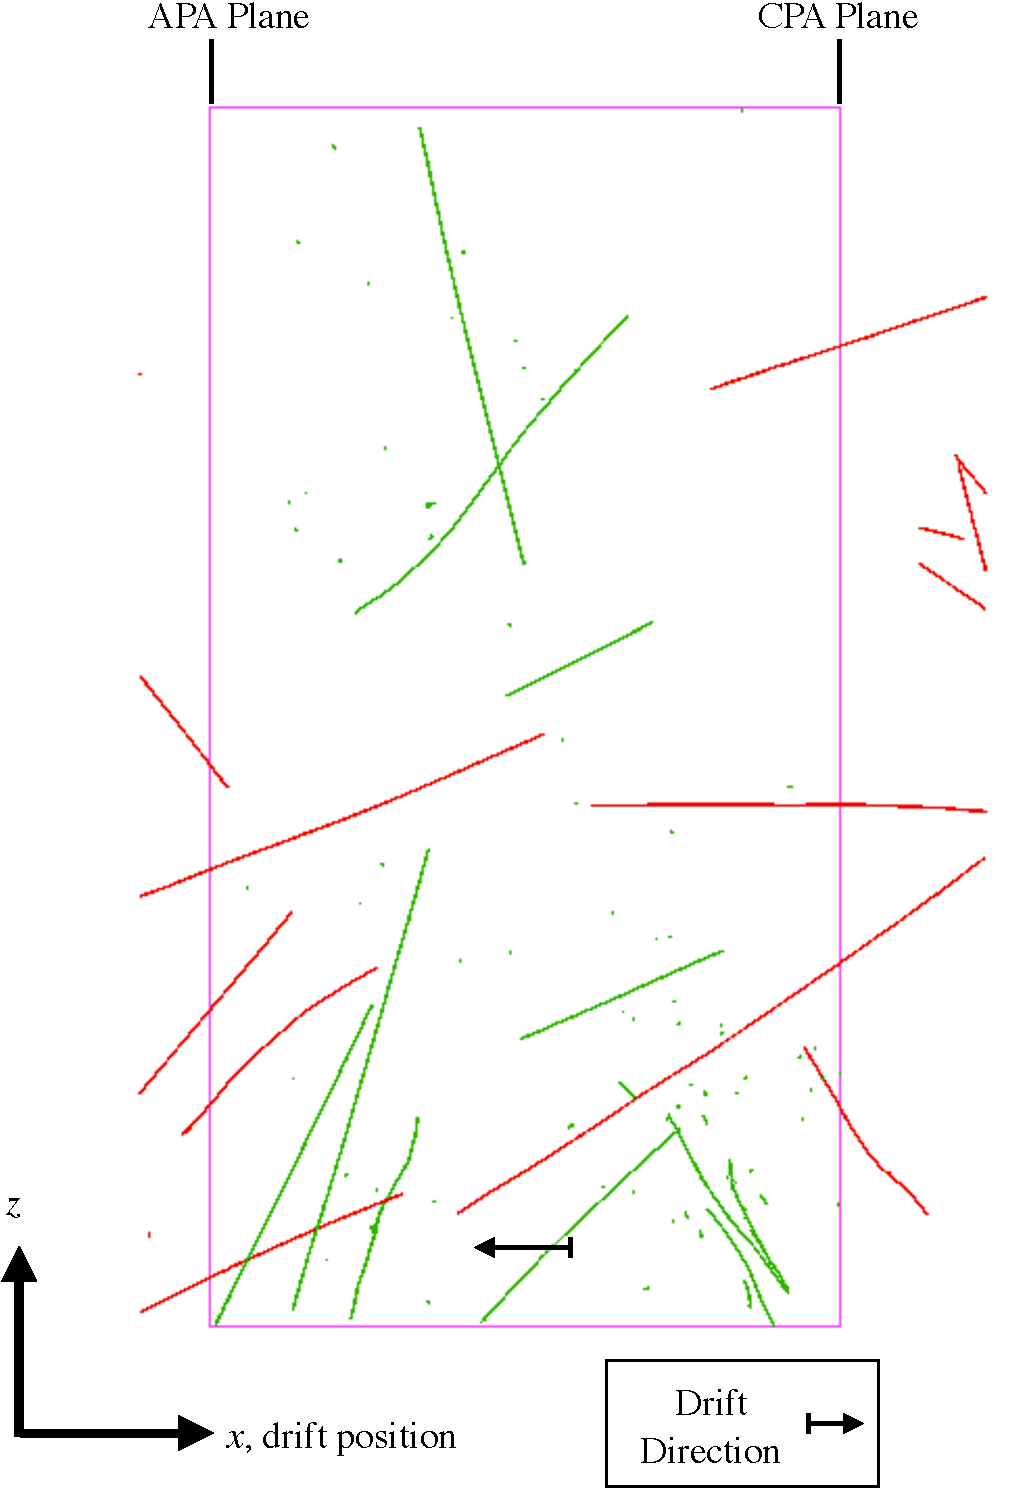
\includegraphics[width=0.28\textwidth]{Figures/Diagram/InTime/InTimeDefinitionXZ.pdf}\label{fig:intimexz}}
\caption{The reconstructed output using the Pandora Cosmic algorithm chain in \protect\subref{fig:intime3d} 3D, \protect\subref{fig:intimexy} the \textit{x-y} plane and \protect\subref{fig:intimexz} the \textit{x-z} plane for a simulated event in ProtoDUNE-SP.  For illustrative purposes only hits appearing in one of the two central drift volumes in ProtoDUNE-SP have been reconstructed.  Particles in red are deemed to be out of time, that is they appear outside the physical boundary of the drift volumes due to an inaccurate offset in the drift position being applied.  Particles in green are those deemed to be in time.  Out of time particles are tagged as cosmic-ray muons.}
\label{fig:intime}
\end{figure}

\begin{figure}
\centering
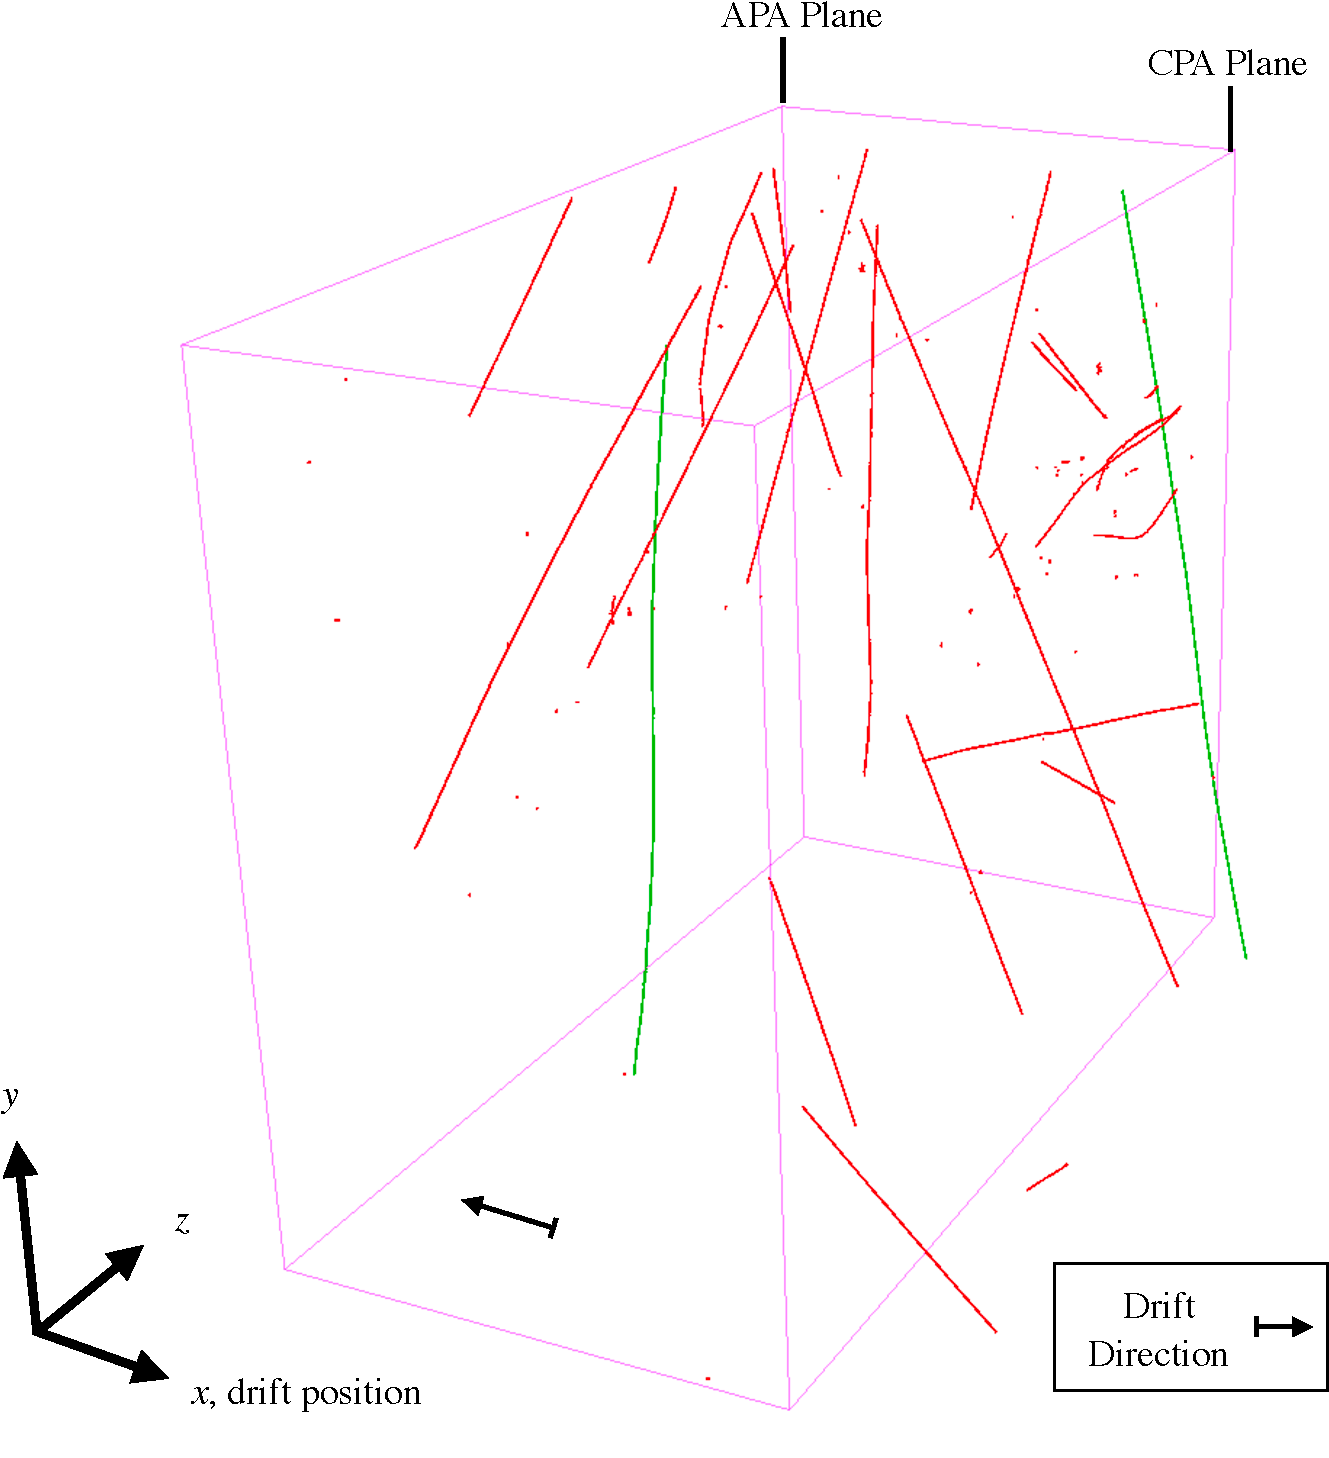
\includegraphics[width=0.3\textwidth]{Figures/Diagram/InTime/TopBottom.pdf}
\caption{The reconstructed output using the Pandora Cosmic algorithm chain in 3D.  For illustrative purposes only hits appearing in one of the two central drift volumes in ProtoDUNE-SP have been reconstructed.  Particles in green are those that have been identified as entering the top face of the detector and exiting the lower face and are tagged as cosmic-ray muons.}
\label{fig:crtopbottom}
\end{figure}

Reconstructed particles identified as clear cosmic-ray muons are then set aside to form one part of the reconstructed event output.  Any input hits not belonging to reconstructed clear cosmic-ray muons form a subset of hits, cosmic-ray muon removed hits, that are then analyzed further.  Other than defining which hits are in the cosmic-ray muon removed hit collection, no information from the initial pass of the Pandora Cosmic algorithm chain is persisted into the remaining reconstruction.  

Following the tagging of reconstructed clear cosmic-ray muons, the cosmic-ray muon removed hits are put through a "slicing" procedure that is designed to group hits together across all three views into regions that contain a single parent particle interaction.  \todo{Picture demonstrating slicing in effect}  Slicing involves running a fast version of the full reconstruction, where particles are reconstructed, but the finesse of particle hierarchies is not considered.  By applying this fast reconstruction, correlations across the three input views are considered when dividing up the event into separate regions, or slices.  This is more powerful than dividing up each view independently.  

For all slices in the event, Pandora Test Beam and Pandora Cosmic algorithm chains are applied to the input hits contained within each slice.  At this stage each slice has two possible reconstructed outputs, based on the test beam and cosmic-ray muon hypotheses respectively.  These reconstruction outputs are then compared in order to determine the most appropriate output to persist.  In ProtoDUNE-SP a BDT is used to drive this decision.  The following features are used as inputs to the boosted decision tree:

\begin{itemize}
\item The eigenvalues of the covariance matrix of the spatial position of the reconstructed 3D hits.
\item The number of reconstructed particles in the slice.
\item The distance of the closest 3D hit to the expected point where the test beam enters the LArTPC.
\item The opening angle between a spatial fit to the 3D hits in a reconstructed particle and the expected direction of the test beam.
\item The vertical distance of the reconstructed 3D hit closest to the top face, high \textit{y}, of the detector.
\end{itemize}

These features are calculated for particles reconstructed using both the Pandora Test Beam and Pandora Cosmic algorithm chains and fed into the BDT.  

The justification for using these features is that the entrance position and direction of the test beam is well understood, cosmic-ray muons typically enter through the top face of the detector and cosmic-ray muons produce highly track oriented topologies in the detector in contrast to typical test beam particle interactions. 

The distribution of the output BDT scores for signal, triggered beam particles, and background, cosmic-ray muons and beam halo, is shown in figure \ref{fig:bdtid} alongside distributions of the selected variables used in the BDT.  There is a clear separation between triggered test beam particles, peaking around a BDT score of zero, and the backgrounds, peaking strongly at minus one.  The distribution of non-triggered particles does have a small peak in the same region as the triggered particles because certain non-triggered beam particles, halo particles from the beam, look topologically similar to signal.  For triggered particles, the supplementary angle to the beam has a narrow peak close to zero, while the cosmic ray distribution is much broader with a peak around $\pi/2$, i.e. the vertical.  The maximum \textit{y} 3D hit position distribution has a tight peak at the top face of the ProtoDUNE-SP detector, $y \approx 600$~cm, while the peak for the triggered beam particles is closer to 400~cm, which is approximately the height of the location where the test beam enters the LArTPC.

Any slice with a BDT score greater than -0.225 is classified as a test beam particle and the Pandora Test Beam reconstruction output is persisted, while all other slices are reconstructed by persisting the Pandora Cosmic hypothesis.  This cut yields a signal efficiency of $99.5 \pm 0.2$\% and a background rejection of $95.3 \pm 0.1$\% in ProtoDUNE-SP simulation.

\begin{figure}
\centering
\subfloat[]{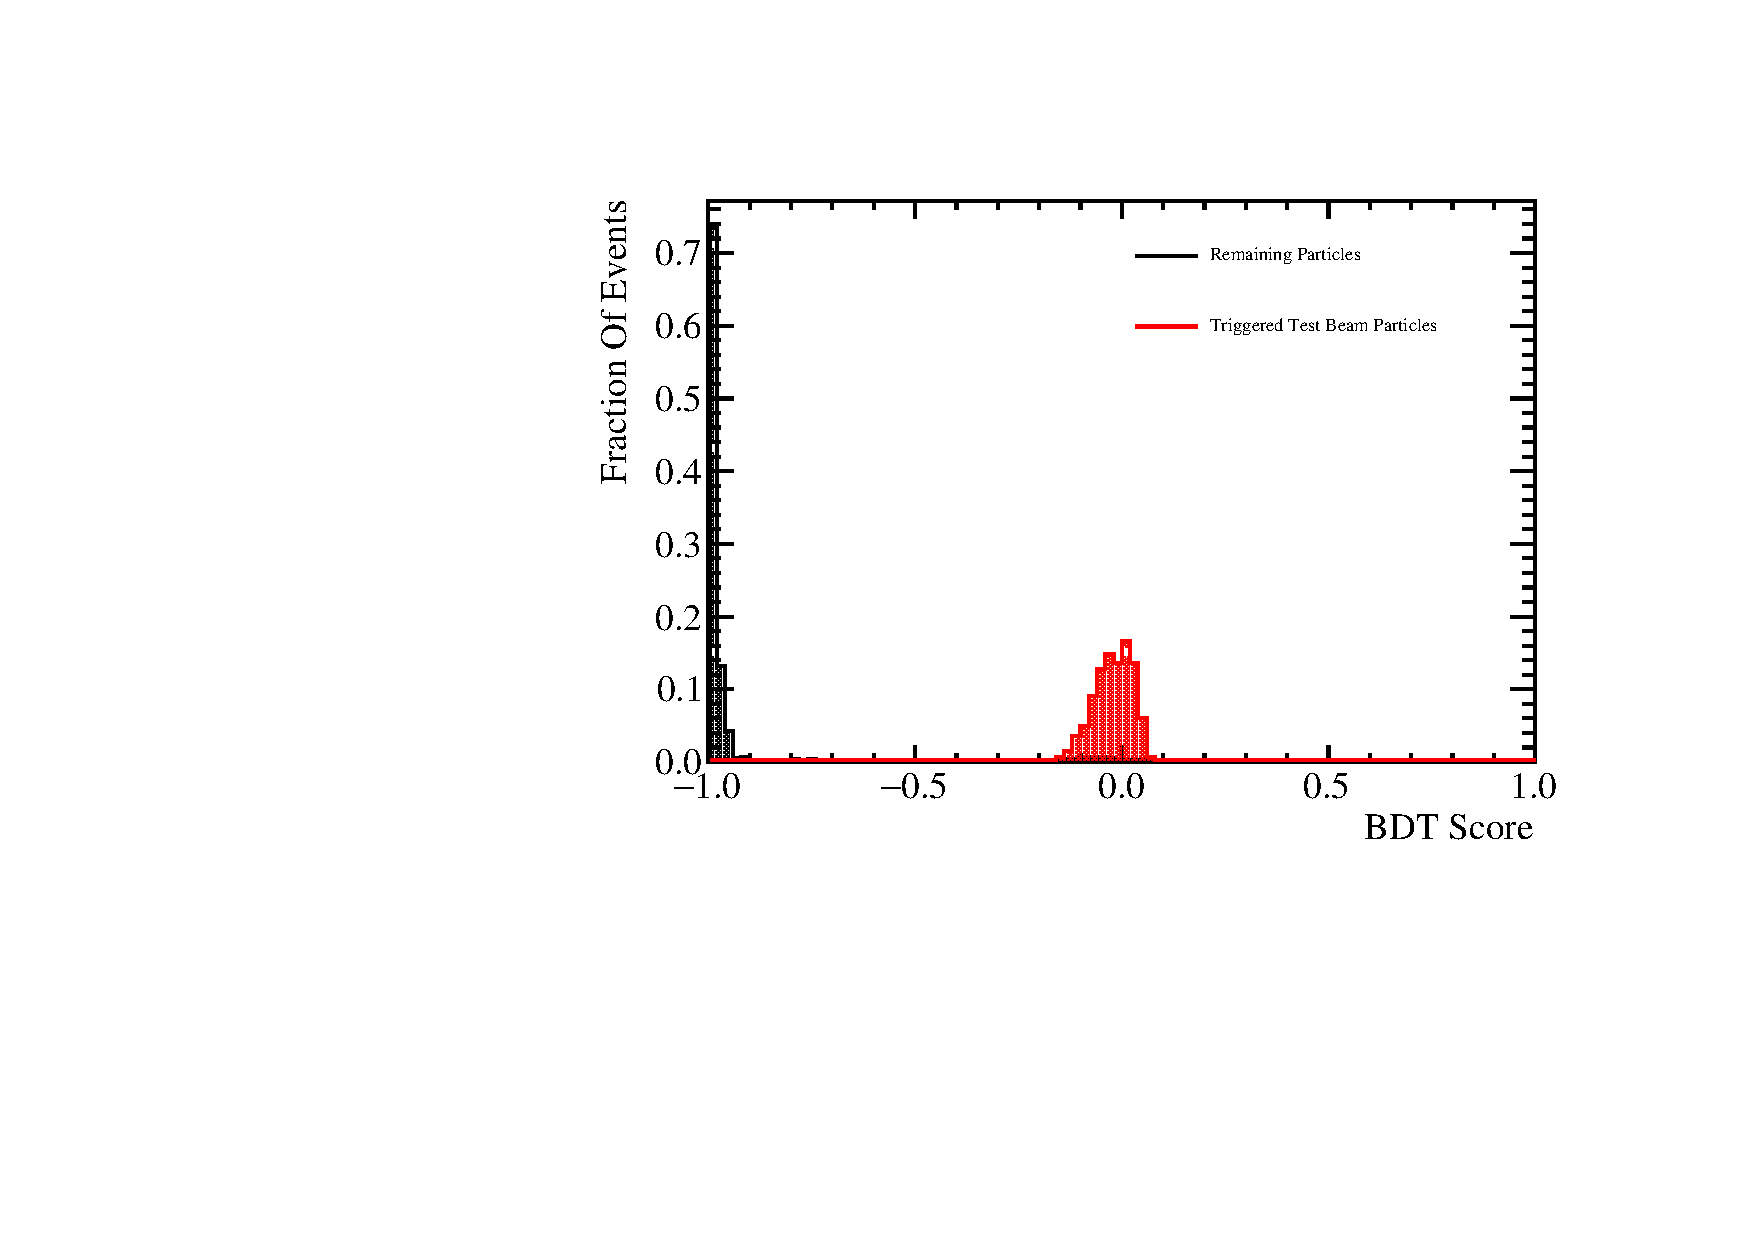
\includegraphics[width=0.75\textwidth]{Figures/TestBeamId/BDTScore.pdf}\label{fig:bdtidscore}} \\
\subfloat[]{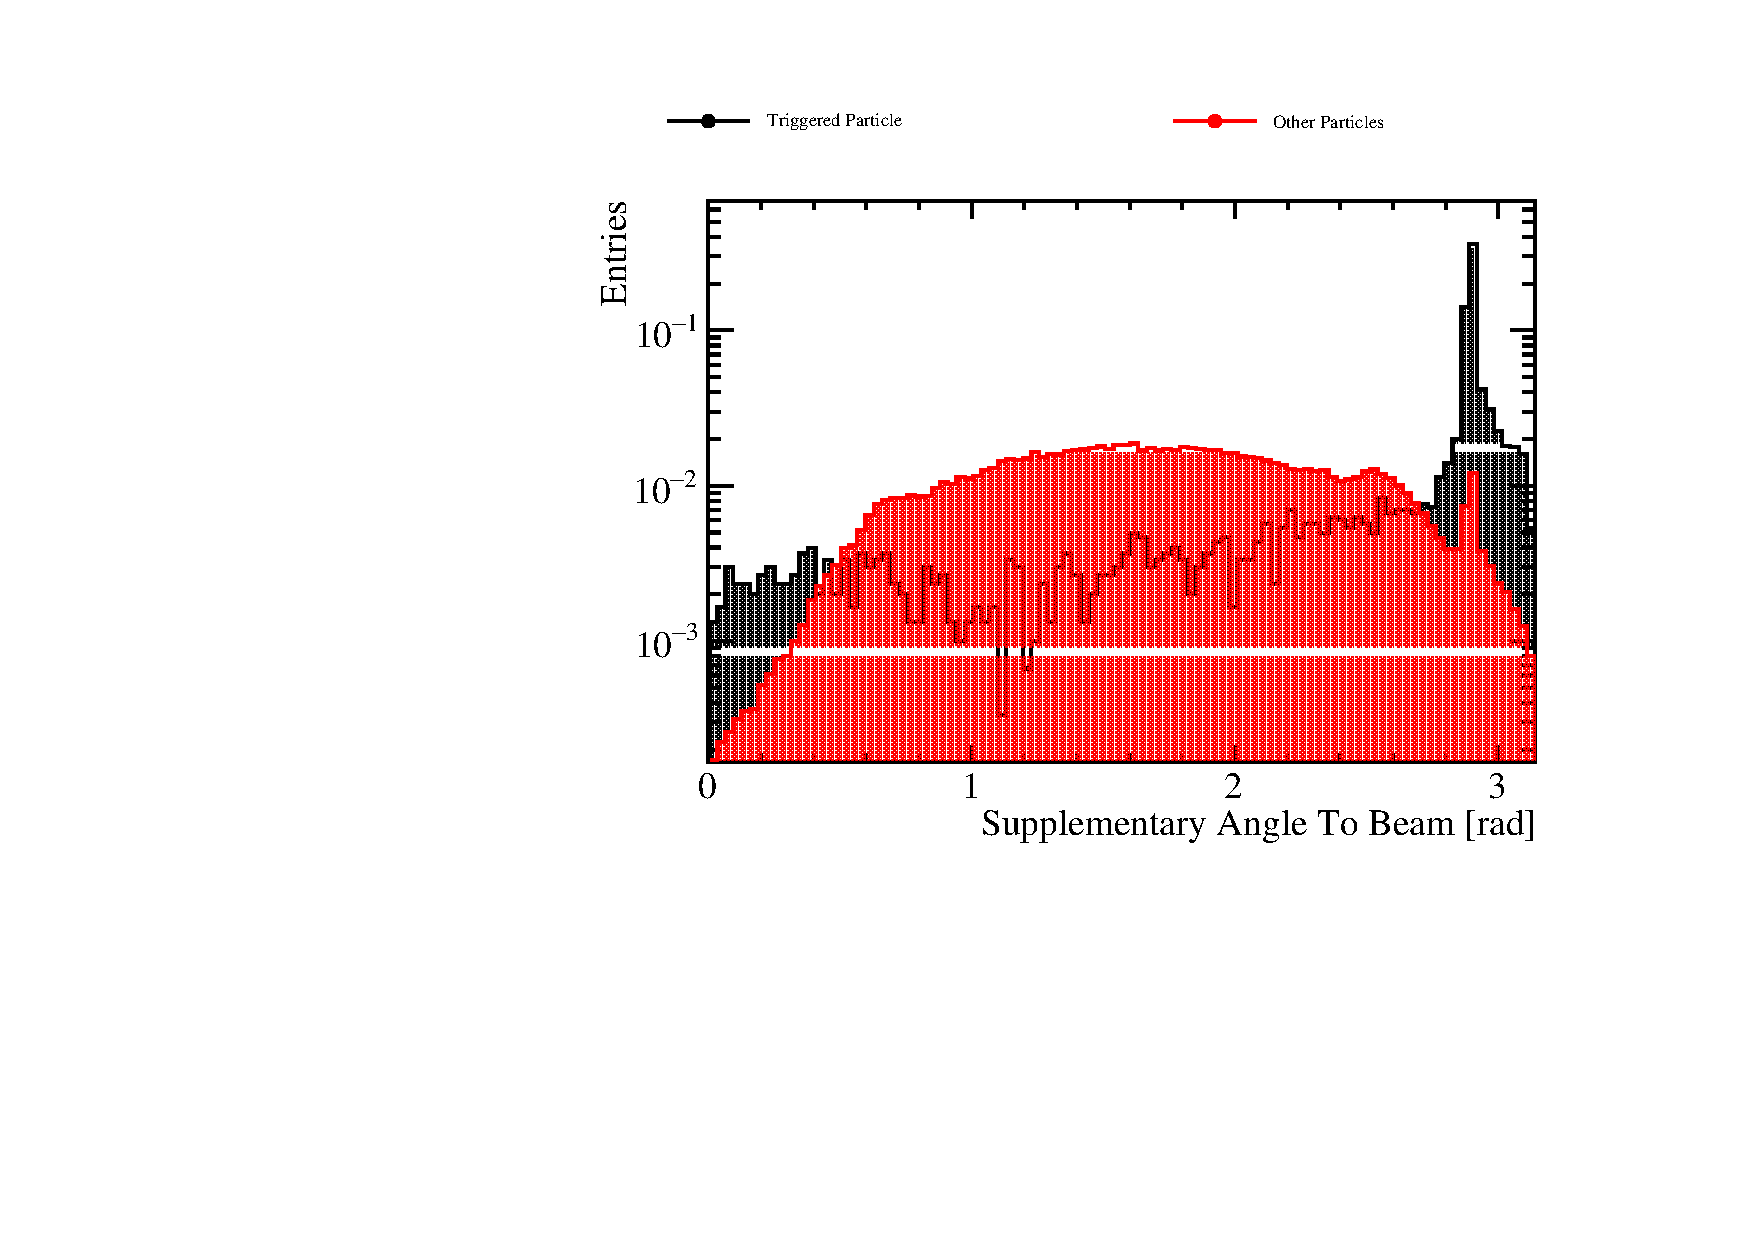
\includegraphics[width=0.5\textwidth]{Figures/TestBeamId/SupplementaryAngleToBeam.pdf}\label{fig:bdtidvar1}}
\subfloat[]{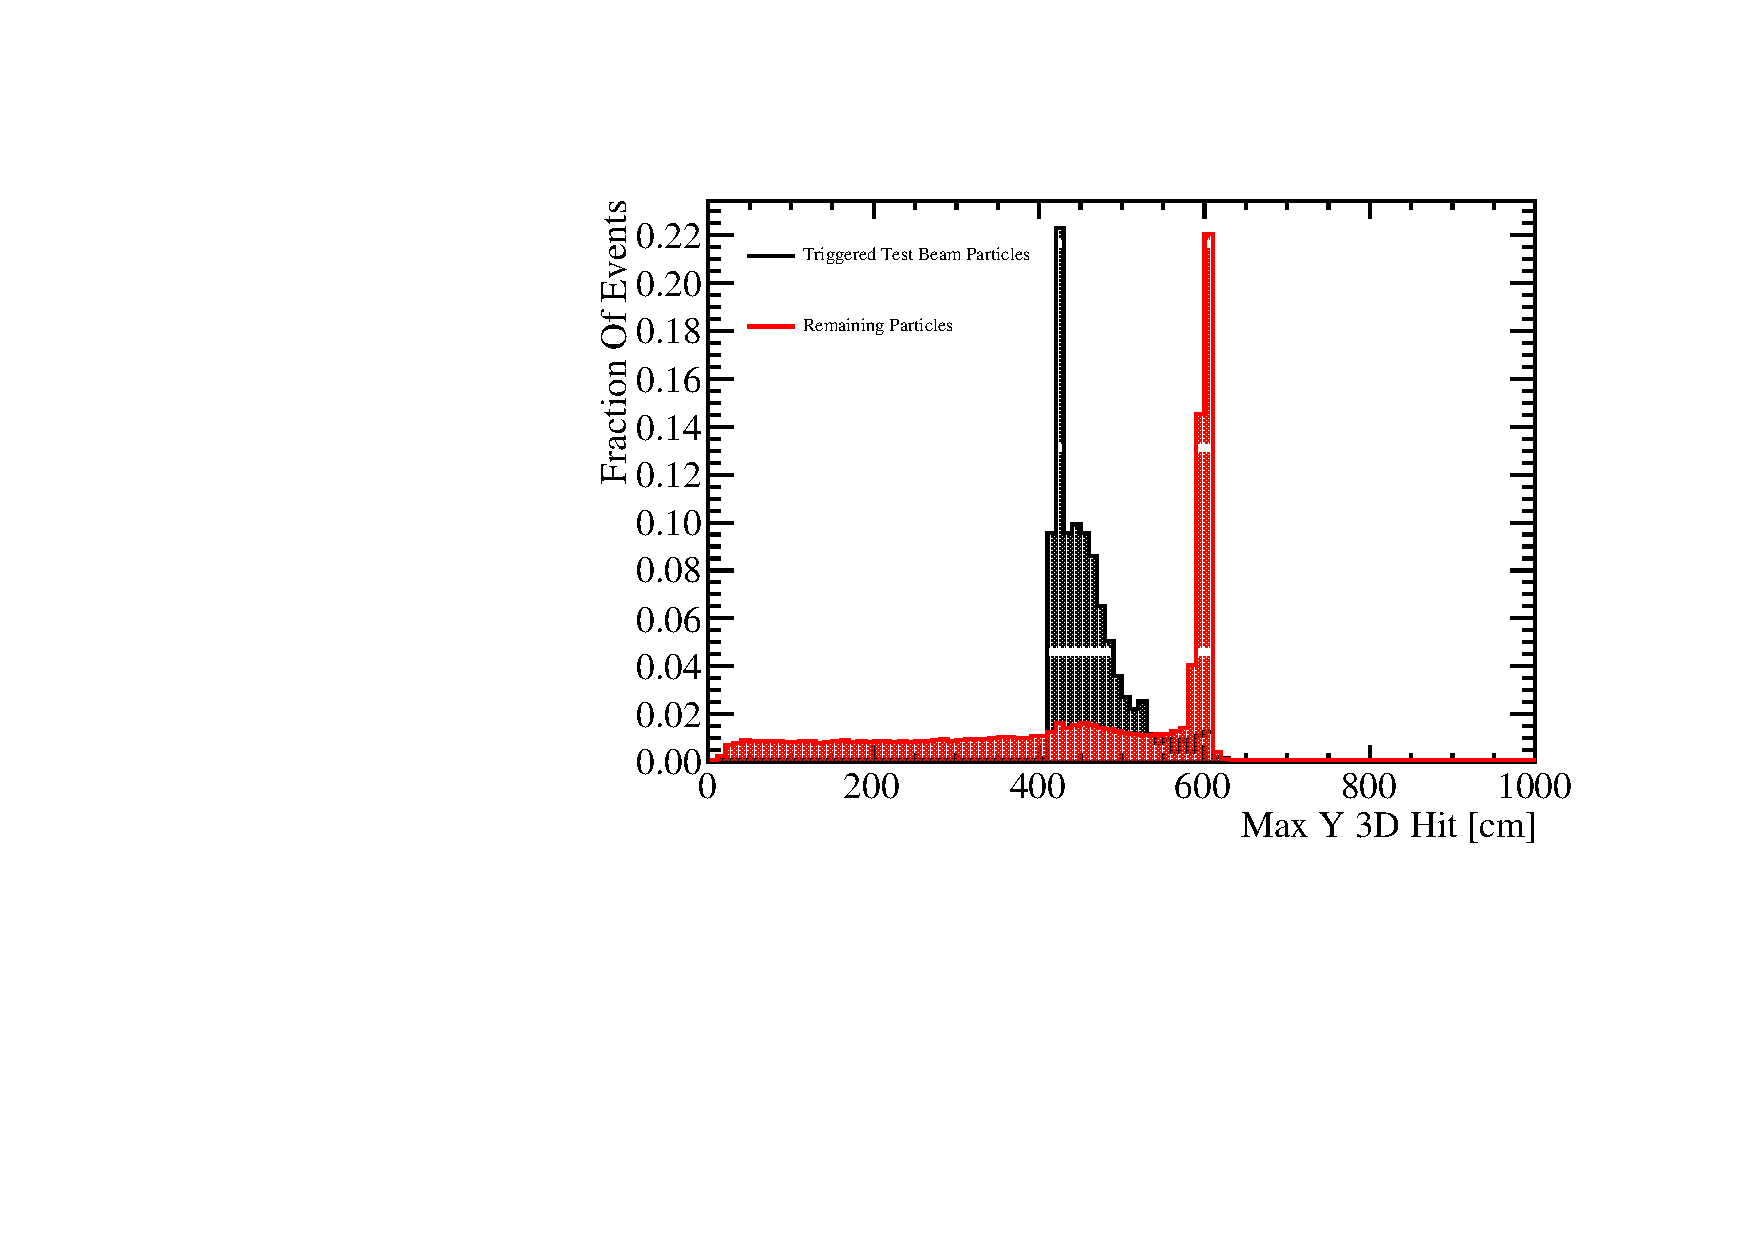
\includegraphics[width=0.5\textwidth]{Figures/TestBeamId/MaxY.pdf}\label{fig:bdtidvar2}}
\caption{Figure \protect\subref{fig:bdtidscore} shows the distribution of the BDT score for triggered test beam particles and all remaining particles.  Figures \protect\subref{fig:bdtidvar1}, and \protect\subref{fig:bdtidvar2} show distributions of selected variables, the supplementary angle to the beam and the max \textit{y} position of any 3D hit in a reconstructed particles respectively, that are used in the test beam identification step.  These variables were calculated using the test beam reconstruction for the slice, however, the corresponding variables obtained using the cosmic-ray muon reconstruction are also propagated into the BDT training step.}
\label{fig:bdtid}
\end{figure}

Figure \ref{fig:examplemcreco} shows an example of the reconstruction output for a simulated ProtoDUNE-SP event, where the test beam particle has been correctly distinguished from the dense cosmic-ray muon background.  Alongside the 3D reconstructed output, this figure also shows the hits identified as being from the test beam particle in the $u$, $v$ and $w$ views.  These 2D views provides a clear demonstration of how correlating features between the three views can help to resolve possible ambiguities that would be present when considering each view independently.  Resolving these ambiguities is a fundamental requirement for being able to determine the particle kinematics in an event.

\begin{figure}
\centering
\subfloat[]{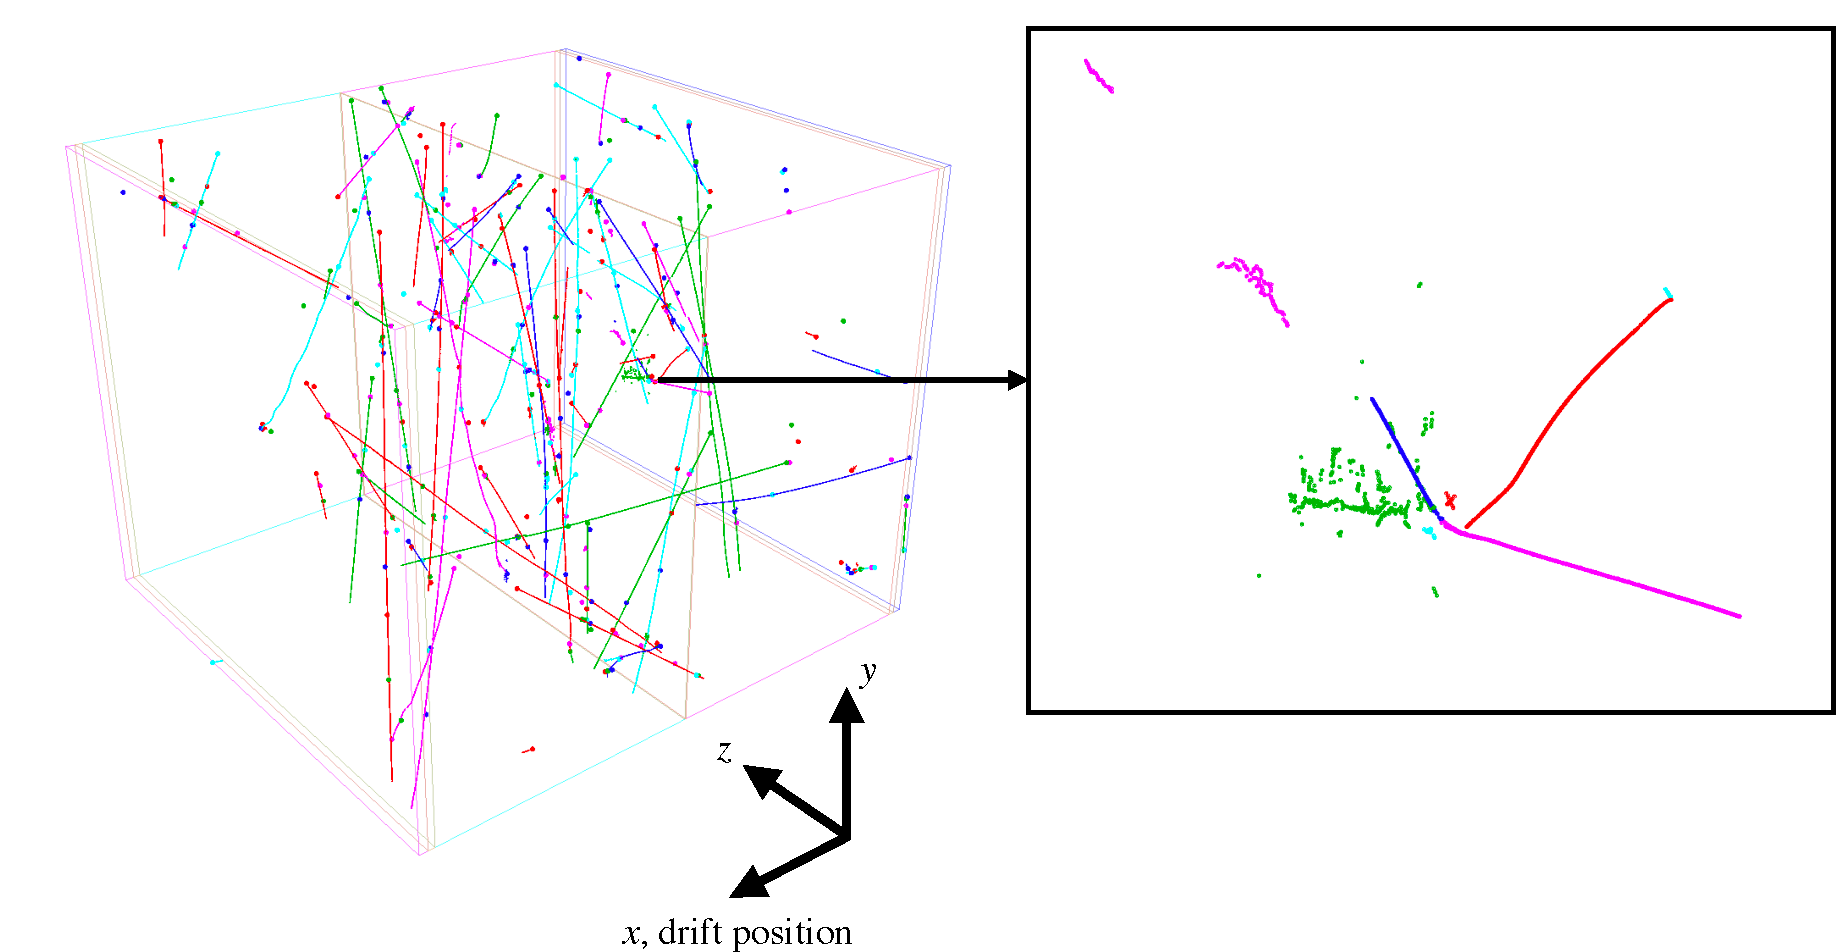
\includegraphics[width=0.75\textwidth]{Figures/EventDisplays/MC/Reconstruction3D.pdf}\label{fig:examplemcrecoa}} \\
\subfloat[]{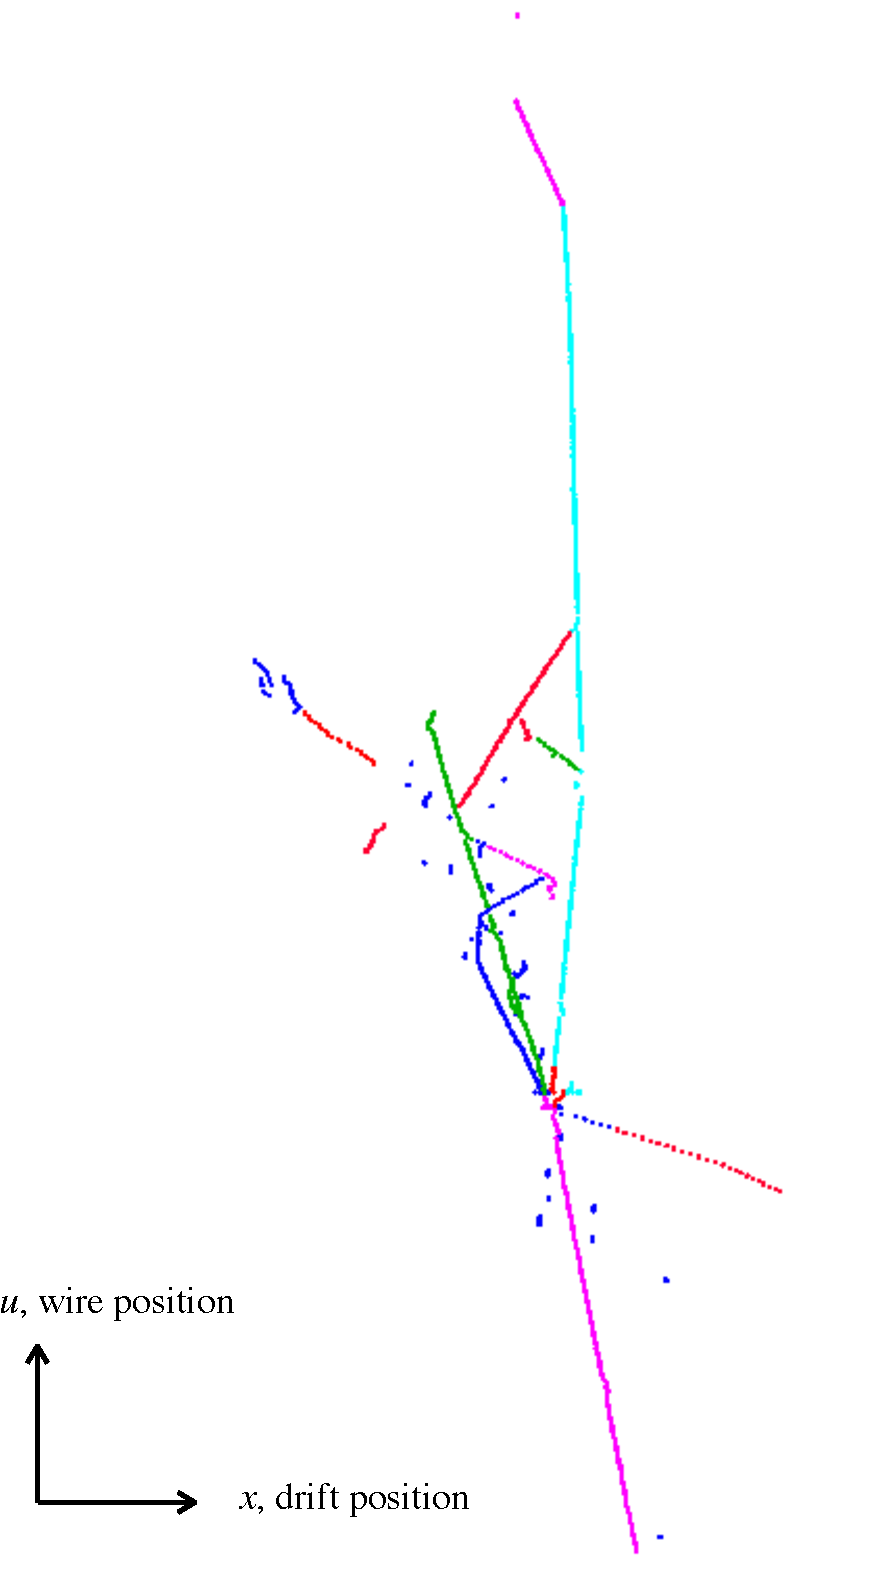
\includegraphics[width=0.29\textwidth]{Figures/EventDisplays/MC/ReconstructionU.pdf}\label{fig:examplemcrecob}}
\subfloat[]{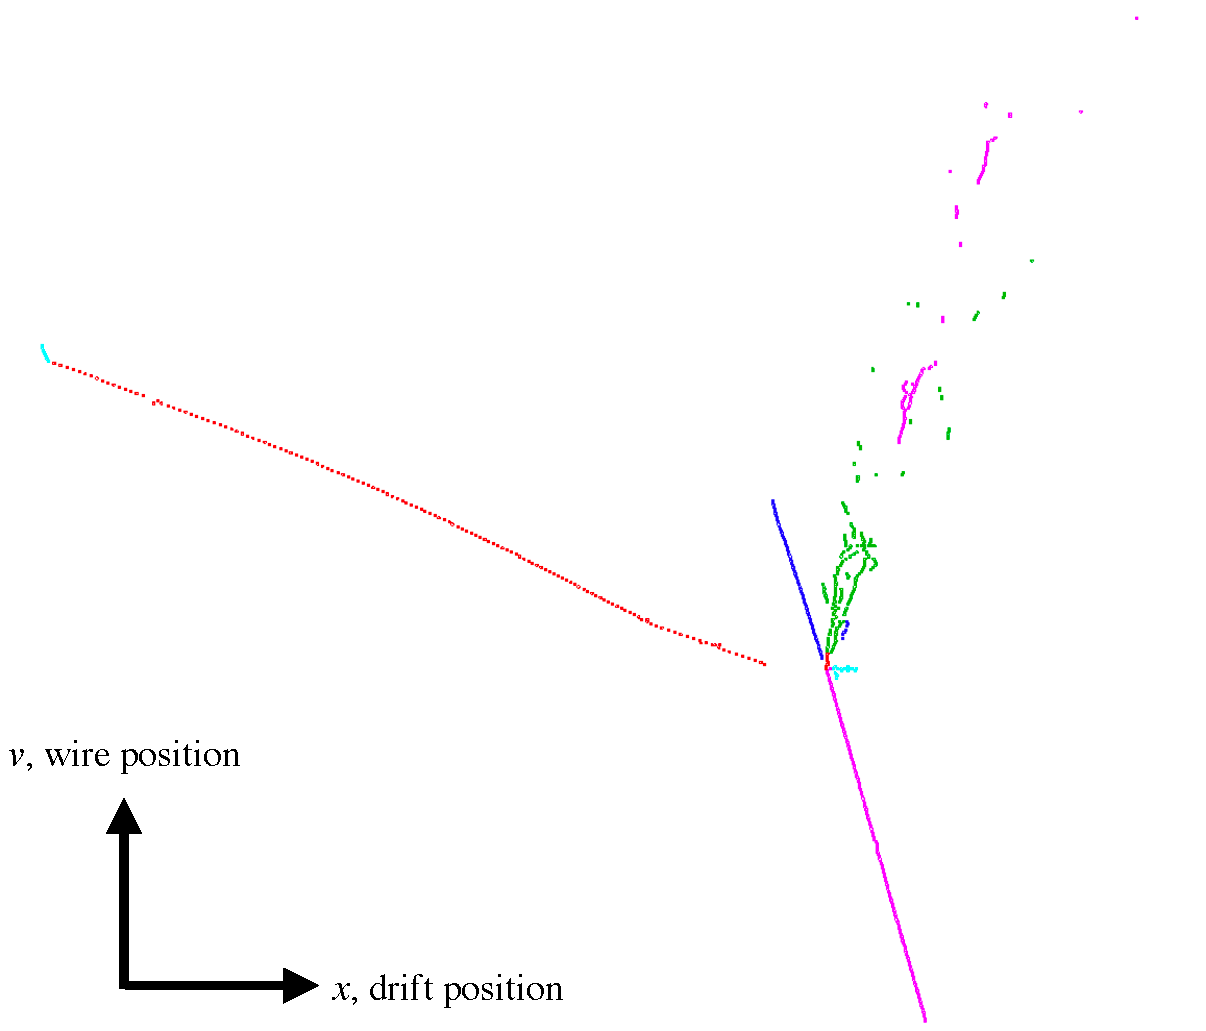
\includegraphics[width=0.34\textwidth]{Figures/EventDisplays/MC/ReconstructionV.pdf}\label{fig:examplemcrecoc}}
\subfloat[]{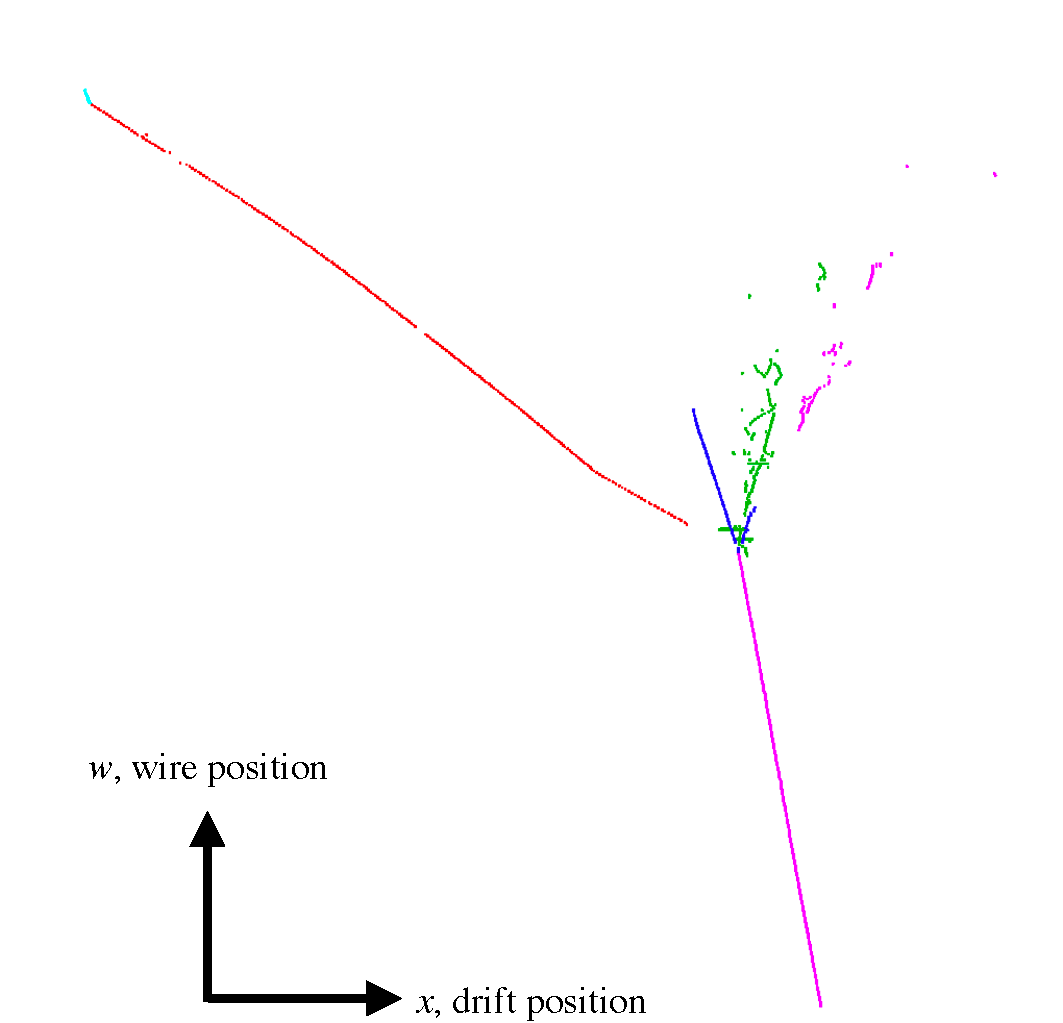
\includegraphics[width=0.3\textwidth]{Figures/EventDisplays/MC/ReconstructionW.pdf}\label{fig:examplemcrecod}} 
\caption{An example of the reconstruction output for a simulated 5~GeV $\pi^{+}$ event at ProtoDUNE-SP.  Figure \protect\subref{fig:examplemcrecoa} shows the 3D reconstruction output, highlighting a reconstructed particle identified as a test beam particle interaction.  Figures \protect\subref{fig:examplemcrecob}, \protect\subref{fig:examplemcrecoc} and \protect\subref{fig:examplemcrecod} show the $u$, $v$ and $w$ view hits respectively for that reconstructed test beam particle.}
\label{fig:examplemcreco}
\end{figure}

\section{Assessment of Pattern Recognition}
\label{sec:assesmentpatrec}

\subsection{Monte-Carlo}
\label{sec:mcmetrics}
For ProtoDUNE-SP a mirrored approach to that taken for evaluating the performance at MicroBooNE was taken \cite{pandorauboone}.  This involves matching Monte-Carlo (MC) particles with reconstructed particles based on the number of shared hits.  

Before evaluating performance metrics, a series of cuts are applied in order to ensure that the MC particles being referenced are "reconstructable", that is they must produce a sufficient number of hits in the LArTPC and must not take the form of an isolated and diffuse topology.  In order for an MC particle to be used in these metrics it must produce at least 15 hits in the detector, with at least 5 hits in at least two of the three views.  Furthermore, MC particle hits produced downstream of a far-travelling neutron, or, if the target particle is track-like, a far-travelling photon, are removed.  This vetoes diffuse topologies originating from particles produced via nuclear excitations. 

Matches between reconstructed and MC particles are made on an event basis by finding the match involving the largest number of shared hits between the reconstructed and MC particle.  Once this match is made the reconstructed and MC particles are declared unavailable, preventing further matches to either being made.  This process is then repeated for all remaining particles in the event.  At this stage all reconstructed and MC particles have at most one match.  Any remaining reconstructed particles that have no match are associated to the MC particle, that by definition must already have a single match, that they share the most hits with irrespective of the number of matches the MC particle currently has.

Once the reconstructed and MC particle matches have been made, the following metrics can be defined:

\begin{itemize}
\item \textbf{Efficiency} : The fraction of MC particles that are matched to at least one reconstructed particle.
\item \textbf{Purity} : The fraction of hits in the reconstructed particle that are shared with the MC particle.
\item \textbf{Completeness} : The fraction of hits in the MC particle that are shared with the reconstructed particle.
\end{itemize}

When MC particles are matched to reconstructed particles, matches are only made if the purity of the match is greater than 50\% in order to ensure that the reconstructed particle is predominantly associated with a single MC particle.  Furthermore, a completeness of 10\% is required in order to veto low quality matches.  These cuts are not applied when reporting the completeness and purity of matches.  

\subsubsection{Test Beam Metrics}
Using the MCC11 ProtoDUNE-SP simulation, the reconstruction of triggered test beam particles was studied.  Table \ref{tab:mcc11species} shows the breakdown of different test beam particle species in this sample.  In order to perform a fair comparison to ProtoDUNE-SP data in following sections, only positively charged triggered test beam particle species are considered.

\begin{table}
\centering
\caption{The number of triggered test beam particle events for the ProtoDUNE-SP MCC11 sample.}
\label{tab:mcc11species} 
\begin{tabular}{cc}
\hline\noalign{\smallskip}
Particle Species & Entries  \\
\noalign{\smallskip}\hline\noalign{\smallskip}
$\pi^{+}$ & 8,874 \\
$e^{+}$ & 6,699 \\
$p$ & 2,164 \\
$K^{+}$ & 452 \\
$\mu^{+}$ & 233 \\
\noalign{\smallskip}\hline
\end{tabular}
\end{table}

Figures \ref{fig:tbrecoeffnhits} show the reconstruction efficiency for the triggered test beam particles as a function of the number of 2D hits in the detector.  As the number of hits in the detector increases, the reconstruction efficiency increases and eventually plateaus around 1,000 hits at $\approx$~80\%.  Inefficiencies in the reconstruction efficiency originate from cosmic-ray muon and beam halo contamination.  If the slice containing the triggered test beam particle contains hits from other sources, then the topological variables used in the test beam particle identification step will be distorted, which can result in the slice being incorrectly classified as a cosmic-ray muon.  Figure \ref{fig:eventdecomp} shows an example of the input hits in \textit{w} view for a simulated event where hits from a triggered test beam particle would be contaminated with those from a beam halo particle due to their close proximity.  

Figure \ref{fig:tbrecoeffbrkdwnnhits} shows how reconstruction efficiency as a function of the number of hits changes when sequentially removing cosmic-ray muons and beam halo from the simulation.  Removing cosmic-ray muons from the simulation increases the reconstruction efficiency of the triggered test beam particle by $\approx 10\%$ uniformly as a function of the number of hits.  Furthermore, removing the beam halo as well yields an additional increase in efficiency of $\approx 10\%$ uniformly as a function of the number of hits.  The remaining failure mode, when both cosmic-ray muons and beam halo have been removed, is the intrinsic inefficiency in the test beam particle identification BDT.  This failure mode occurs when a slice containing a triggered beam particle has topological properties that differ significantly from what is expected by the BDT.  This predominantly occurs for particles that produce a small number of hits in the detector because the precision on the topological properties used by the BDT degrades as the number of hits used for calculating the properties decreases.  

Figure \ref{fig:tbrecoeffp} show the reconstruction efficiency for the triggered test beam particles as a function of the momentum of the particle.  The reconstruction efficiency as a function of the test beam particle momentum increases from 87.5\% at 1~GeV to 92.7\% at 3~GeV before falling to 75.4\% at 7~GeV.  At low beam momenta, the number of hits in the triggered test beam particle is low resulting in more inaccurate topological variables being fed into the test beam identification BDT and the lower efficiency.  At high beam momentum, the affect of beam halo contamination dominates the efficiency.  

Figure \ref{fig:tbrecoeffbrkdwnp} shows the impact on the reconstruction efficiency as a function of momentum of removing cosmic-ray muons and beam halo from the simulation.  Removing the comsic-ray muon background improves the efficiency by approximately $\approx 10\%$ uniformly as a function of momentum.  Removing the beam halo in addition to this results in a gain in reconstruction efficiency of $\approx 10\%$ at 1~GeV, almost no gain at 3~GeV and a significant gain of almost $\approx 20\%$ at 7~GeV.  This indicates that the affect of beam halo contamination grows as a function of triggered test beam momenta and that, at high high test beam momenta, it is the dominate source of error in the reconstruction efficiency.  

Figures \ref{fig:tbrecopur} and \ref{fig:tbrecocomp} show the purity and completeness of the reconstructed test beam particle respectively.  Both of these distributions have a strong peak at one, indicating that the triggered test beam particle is being reconstructed as a single complete particle.  There are low value tails in both of these distributions; 14.9\% of events have a purity of less than 80\% and 14.6\% of events have completeness of less than 80\%.  A low value of purity indicates that hits from separate primary MC particles have been merged together.  The effects of contamination, whether from cosmic-ray muons or beam halo, will degrade the triggered test beam particle purity.  Any deviation from unity in the completeness indicates that the triggered test beam particle has been split into several reconstructed particles.  An example of this is given in figure \ref{fig:completenessfig}, which shows the reconstruction output in the \textit{w} view for a simulated 7~GeV $\pi^{+}$ event without cosmic-ray muon and beam halo contamination.  

Figure \ref{fig:tbrecoeffbrkdwnpur} and \ref{fig:tbrecoeffbrkdwncomp} show the effect of sequentially removing cosmic-ray muons and beam halo from the simulation on the purity and completeness respectively.  Removing the cosmic-ray muons improves both the purity and completeness resulting in 5.6\% of events have a purity of less than 80\% and 6.7\% of events have completeness of less than 80\%.  This improvement is expected as hits from cosmic-ray muons will no longer be contaminating the reconstructed beam slice leading to a higher purity.  Furthermore, the completeness also improves because the slicing algorithms will be less active without the cosmic-ray muon hits to seed the creation of new slices.  This means the triggered test beam particle is less likely to be split into different slices that would result in a lower completeness.  Removing both cosmic-ray muons and beam halo leads to all particles having a purity of 100\%, because all possible sources of contamination have been removed.  In comparison to the effect of removing cosmic-ray muons, the completeness change when also removing beam halo from the simulation is negligible.  This is to be expected as there are significantly more primary MC particles per event originating from cosmic-ray muons than from beam halo.  This results in the slicing algorithm, a source of incomplete triggered test beam particles, becoming far less active for events where comsic-ray muons have been removed irrespective of the presence of the second order small beam halo affect.

\begin{figure}
\centering
\subfloat[]{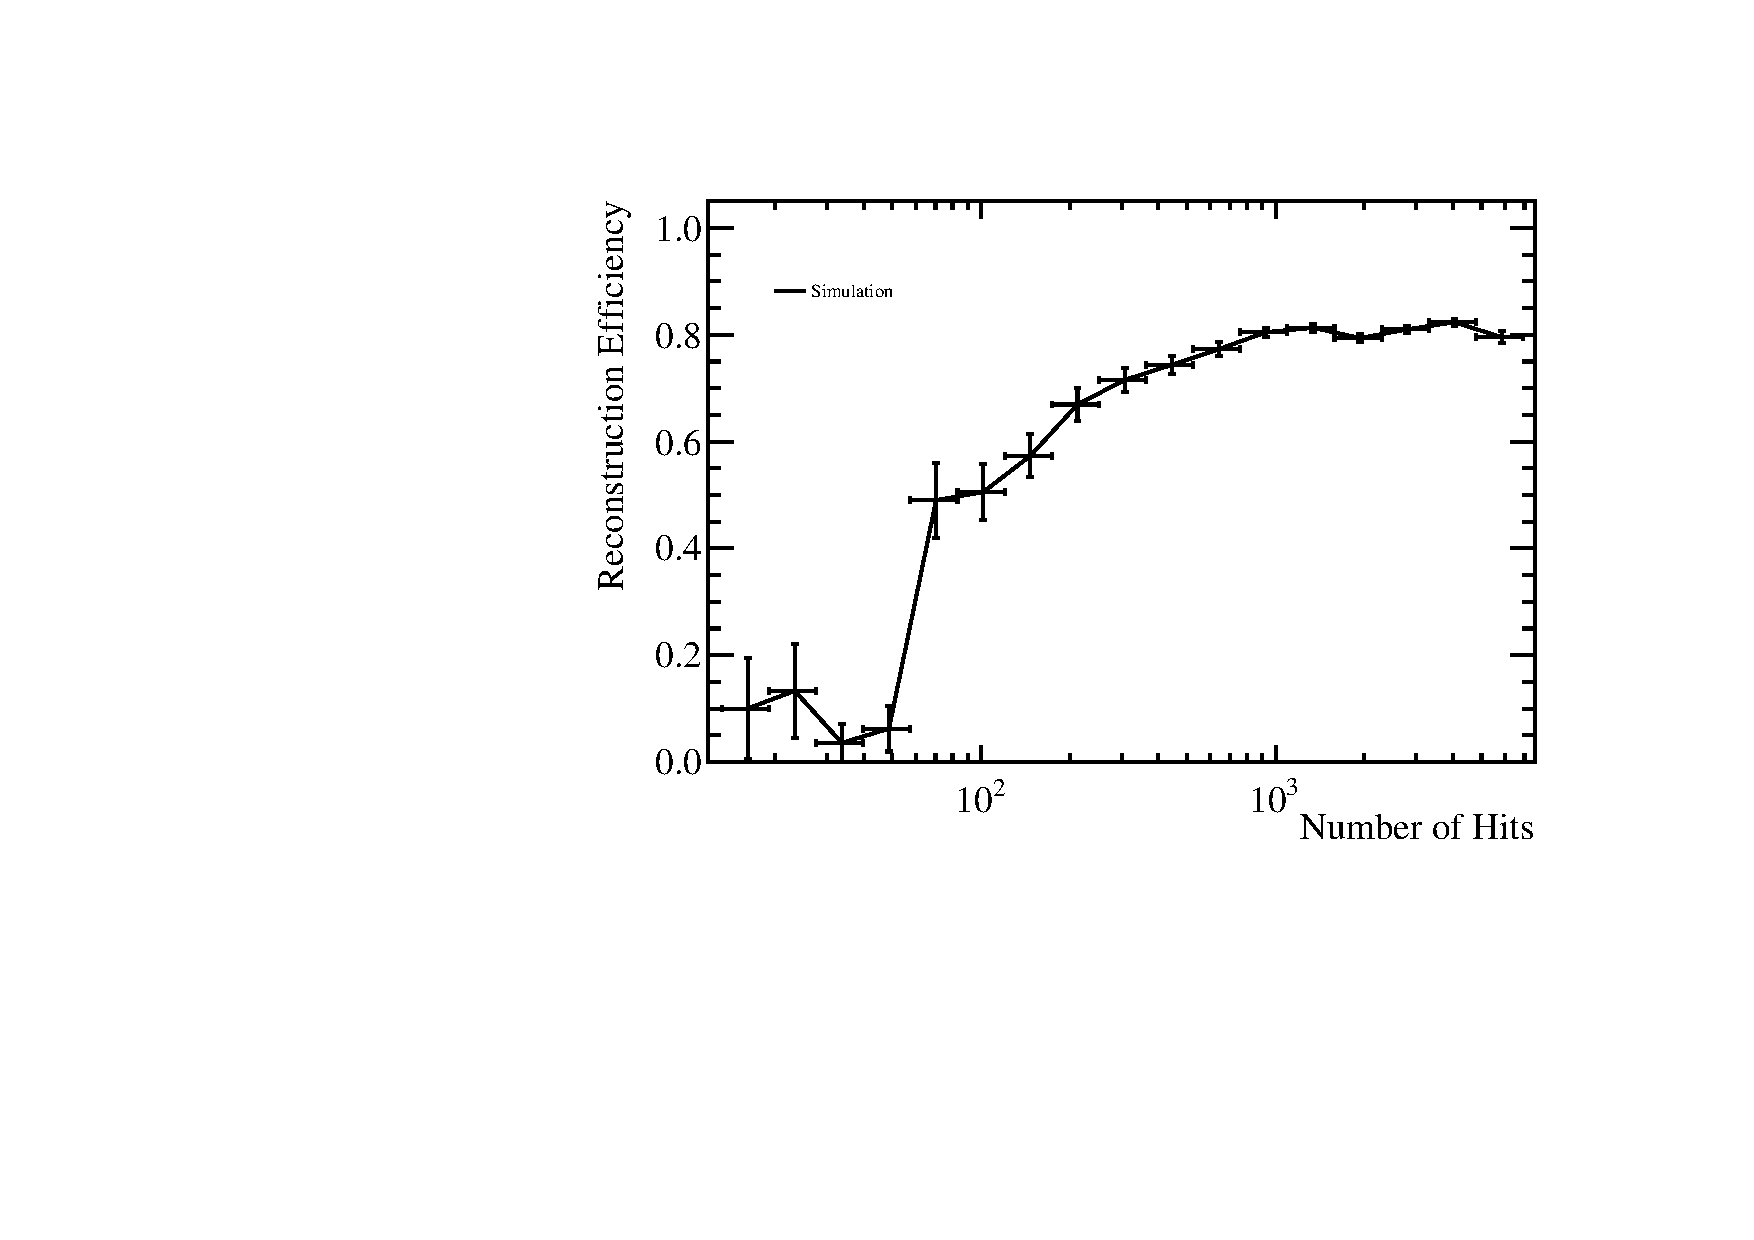
\includegraphics[width=0.45\textwidth]{Figures/Metrics/MC/Beam/BeamParticleEfficiencyVsNHits.pdf}\label{fig:tbrecoeffnhits}}
\subfloat[]{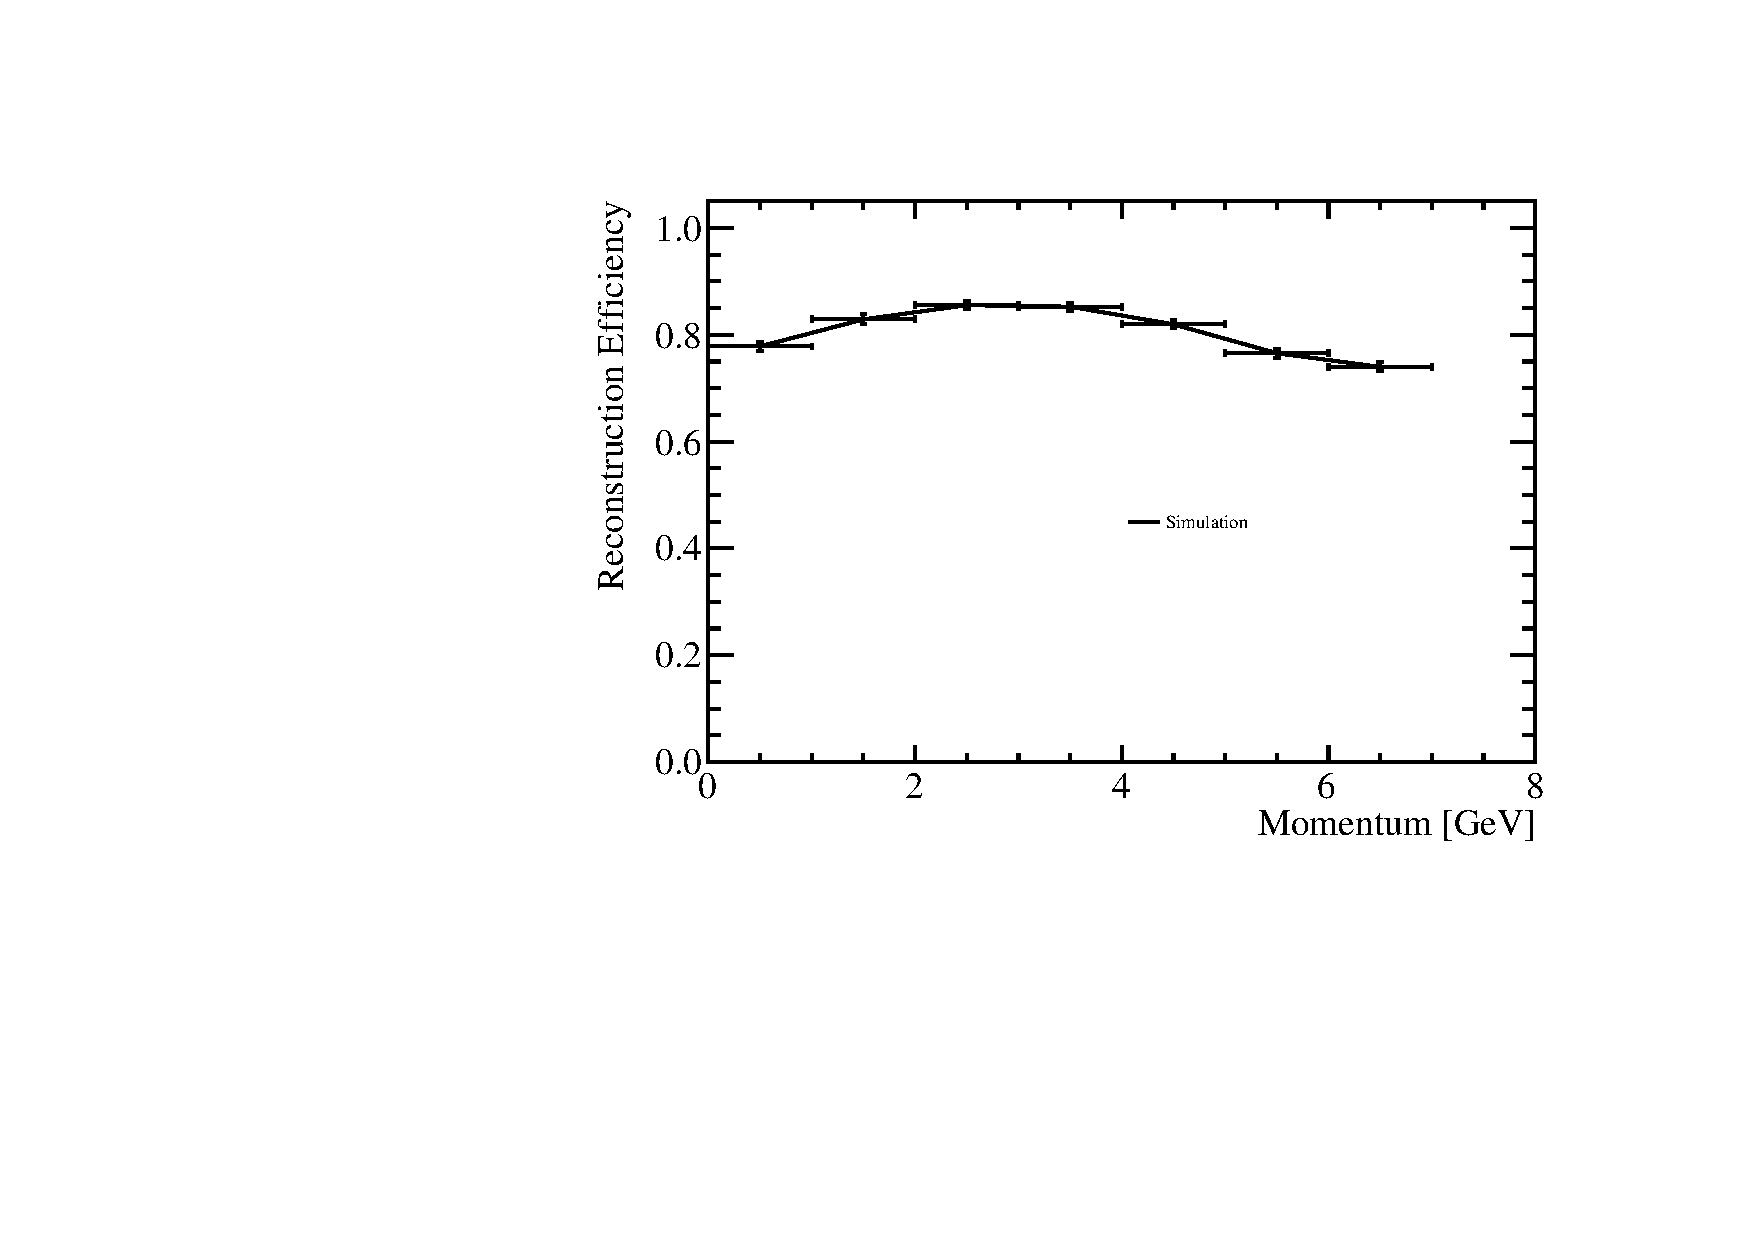
\includegraphics[width=0.45\textwidth]{Figures/Metrics/MC/Beam/BeamParticleEfficiencyVsMomentum.pdf}\label{fig:tbrecoeffp}} \\
\subfloat[]{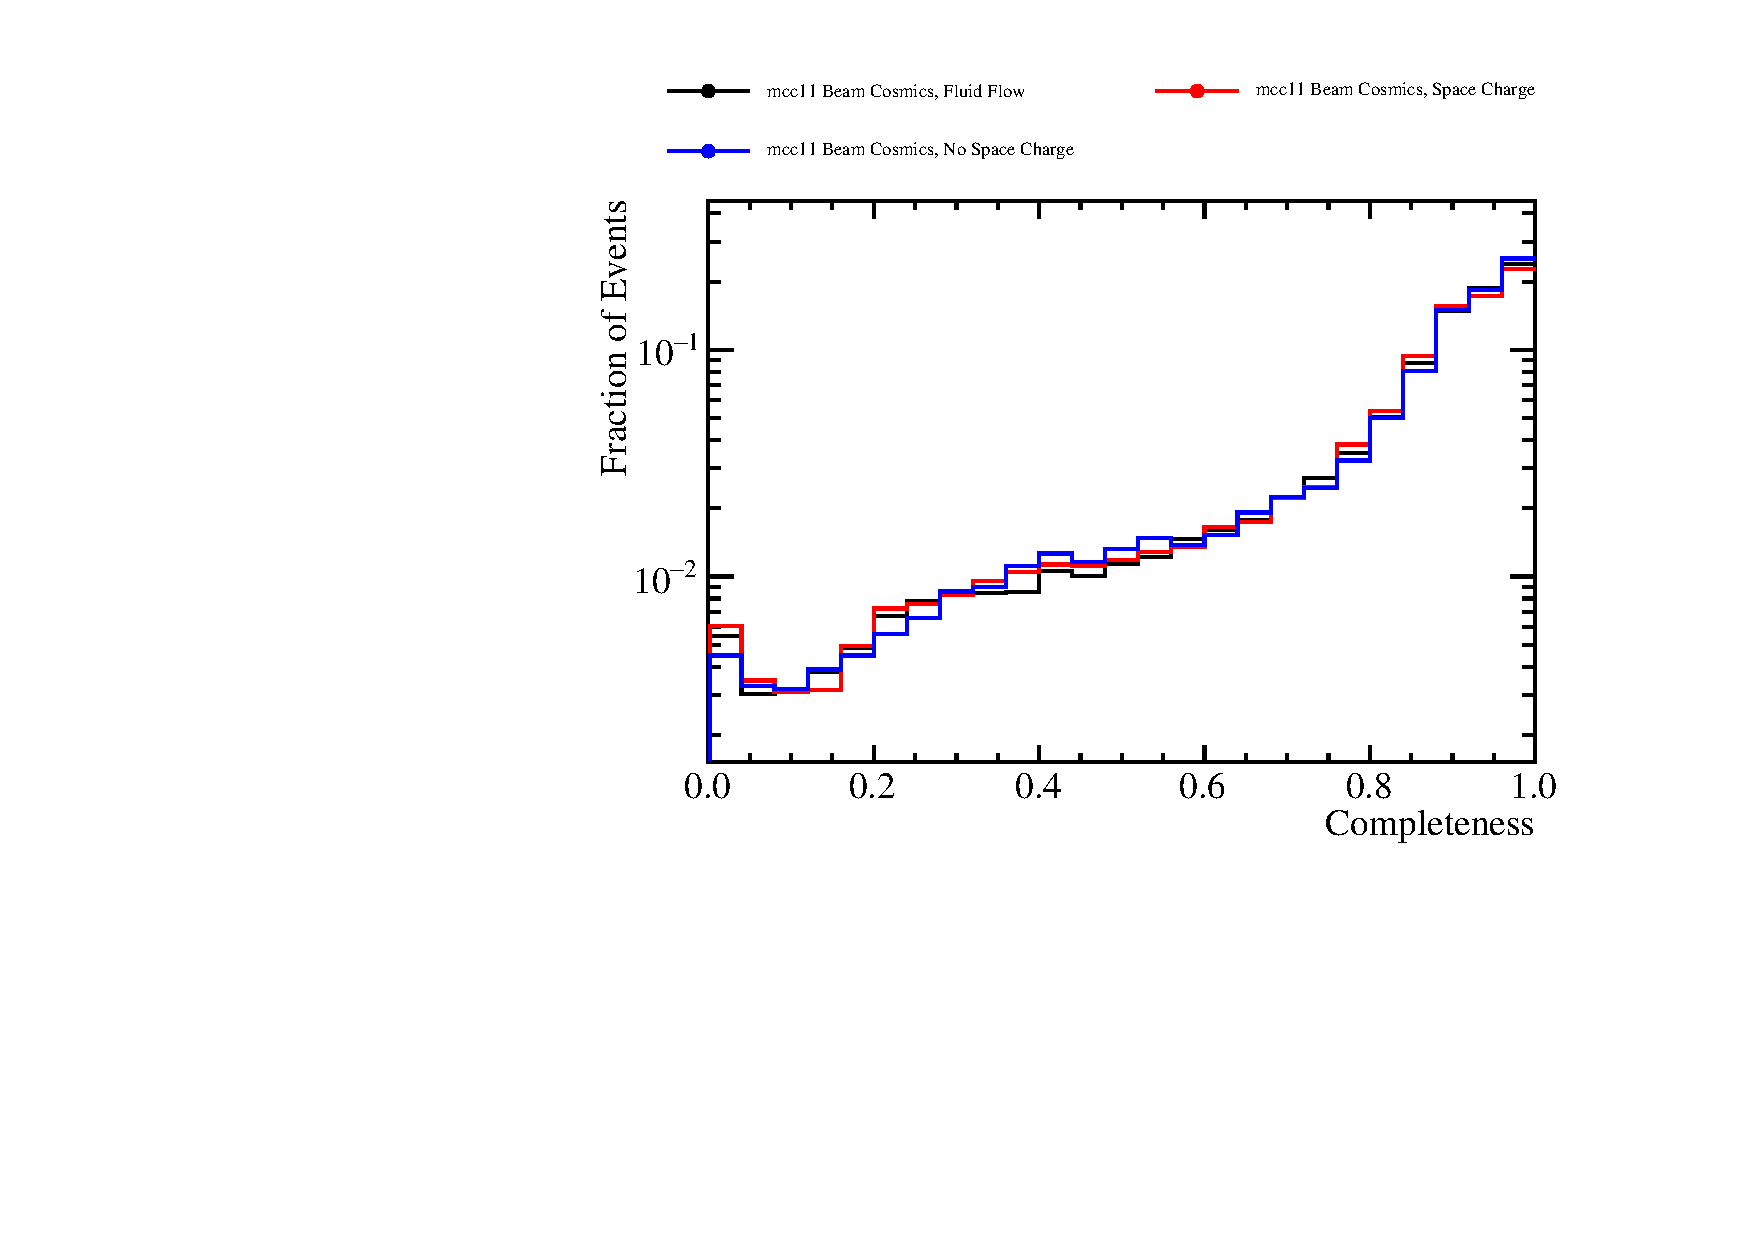
\includegraphics[width=0.45\textwidth]{Figures/Metrics/MC/Beam/BeamParticleCompleteness.pdf}\label{fig:tbrecocomp}}
\subfloat[]{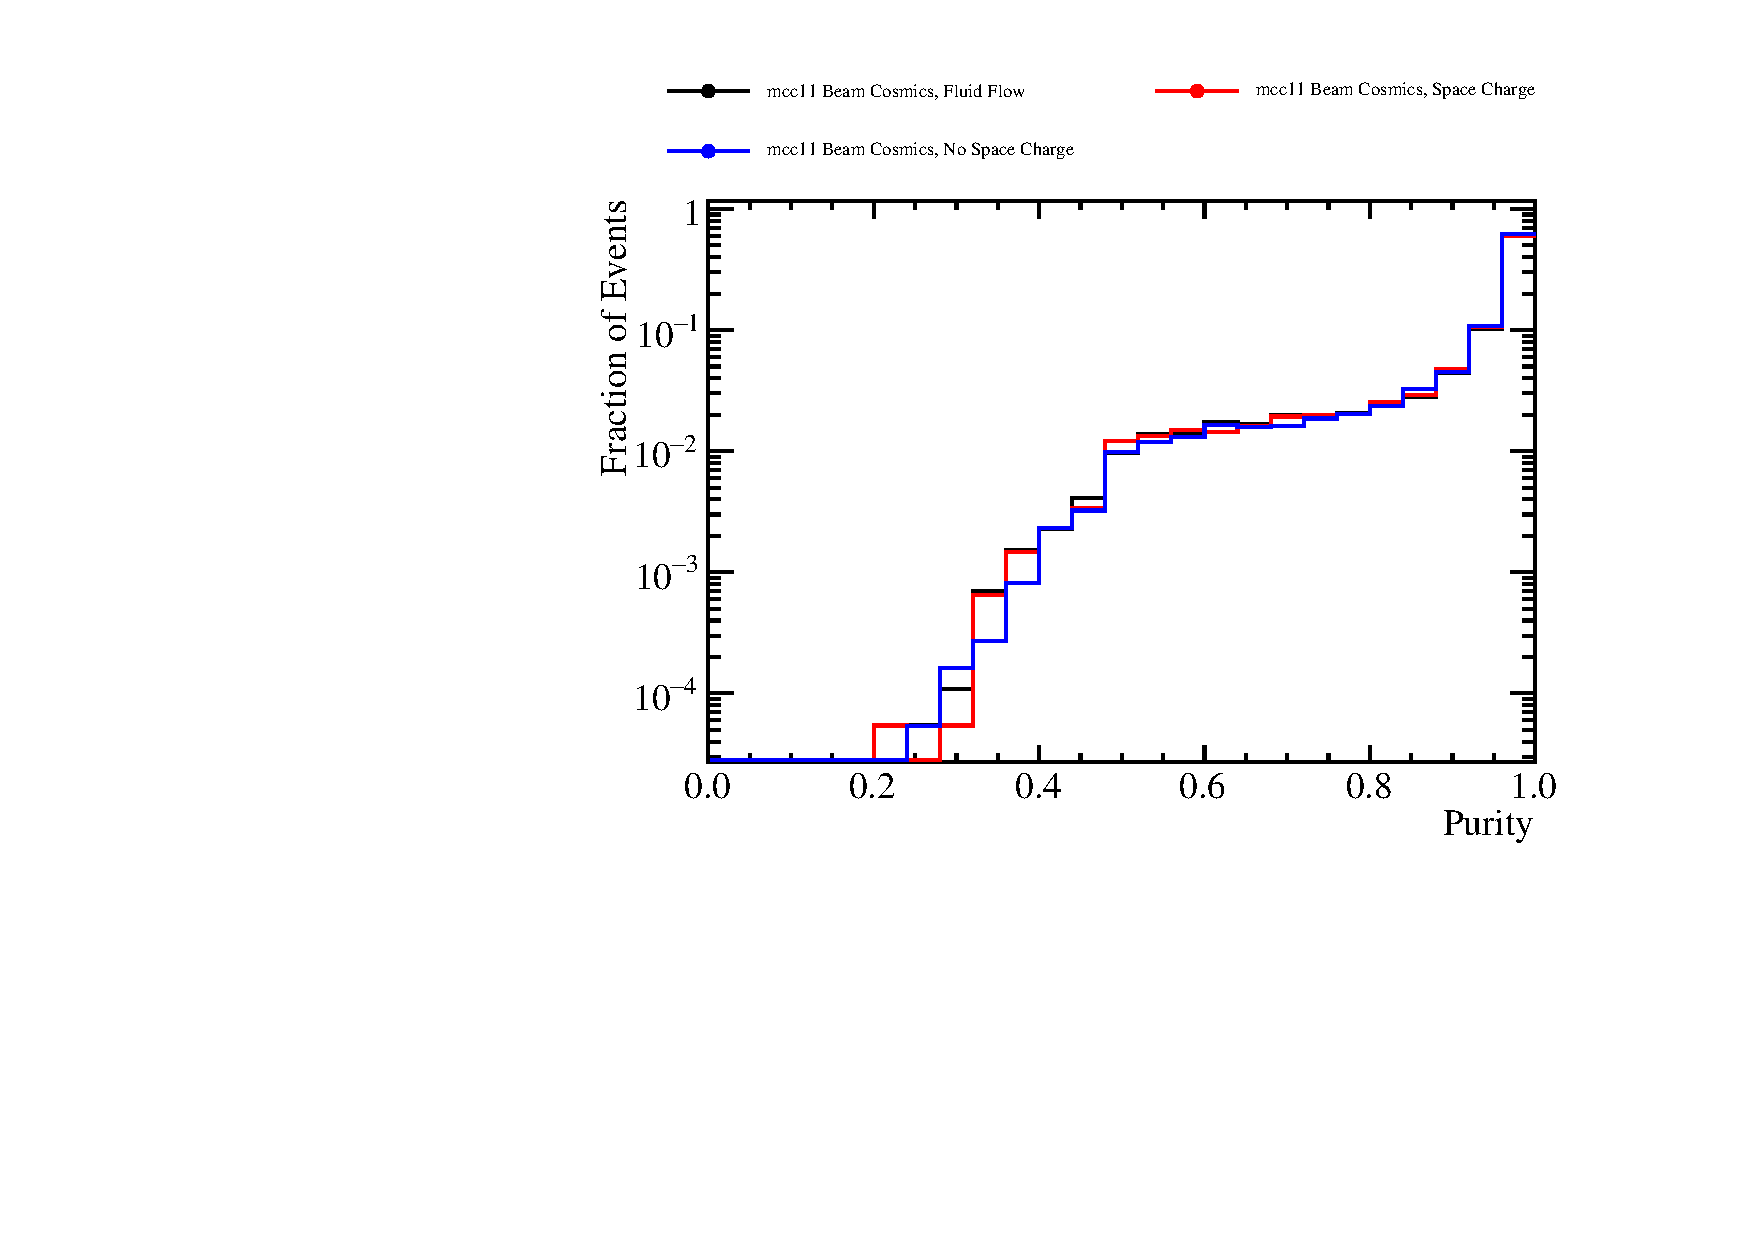
\includegraphics[width=0.45\textwidth]{Figures/Metrics/MC/Beam/BeamParticlePurity.pdf}\label{fig:tbrecopur}}
\caption{The test beam particle reconstruction efficiency as a function of \protect\subref{fig:tbrecoeffnhits} the number of hits produced by the test beam particle and \protect\subref{fig:tbrecoeffp} the momentum of the test beam particle in simulation.  The error bars on the reconstruction efficiency show the statistical error.  Figures \protect\subref{fig:tbrecocomp} and \protect\subref{fig:tbrecopur} show the completeness and purity of the reconstructed test beam particle.}
\label{fig:tbrecoeff}
\end{figure}

\begin{figure}
\centering
\subfloat[]{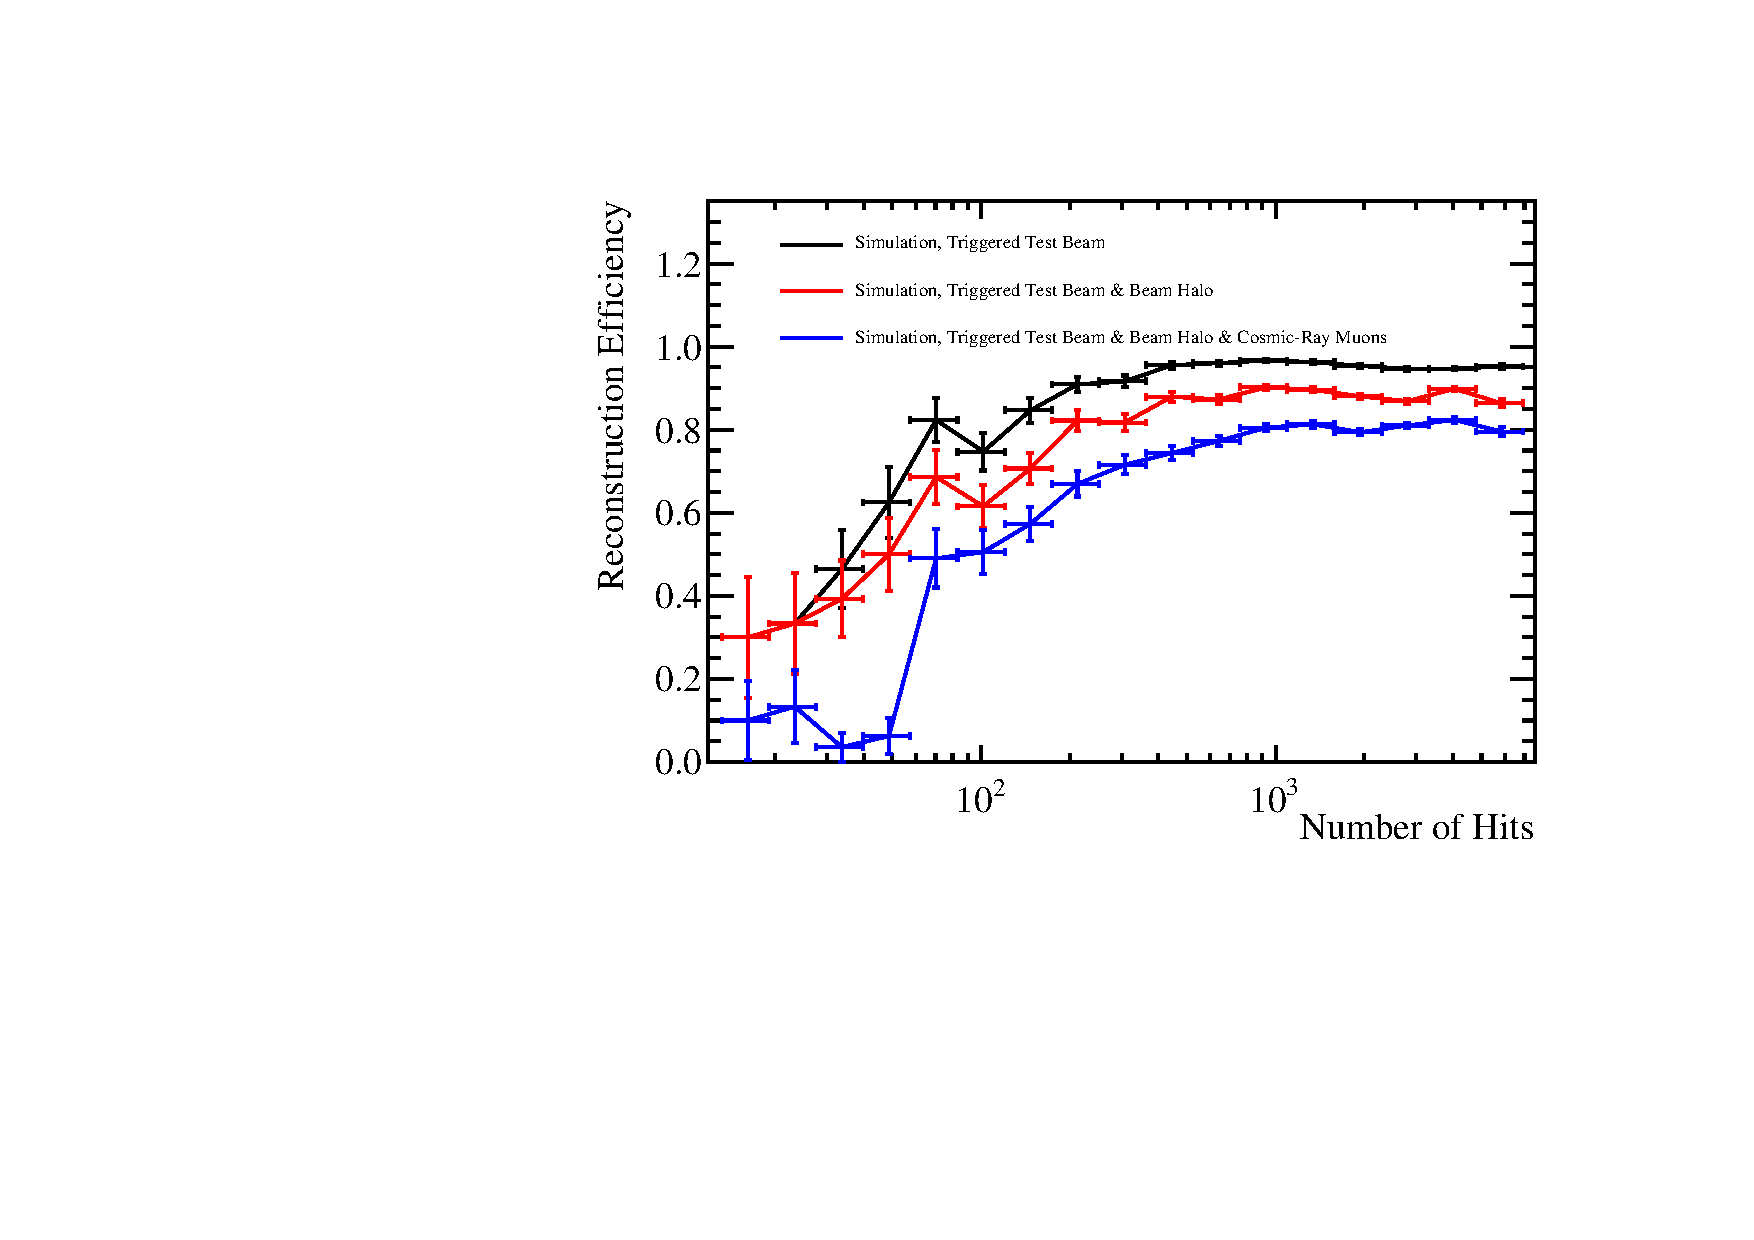
\includegraphics[width=0.45\textwidth]{Figures/Metrics/MC/Beam/Breakdown/BeamParticleEfficiencyVsNHits.pdf}\label{fig:tbrecoeffbrkdwnnhits}}
\subfloat[]{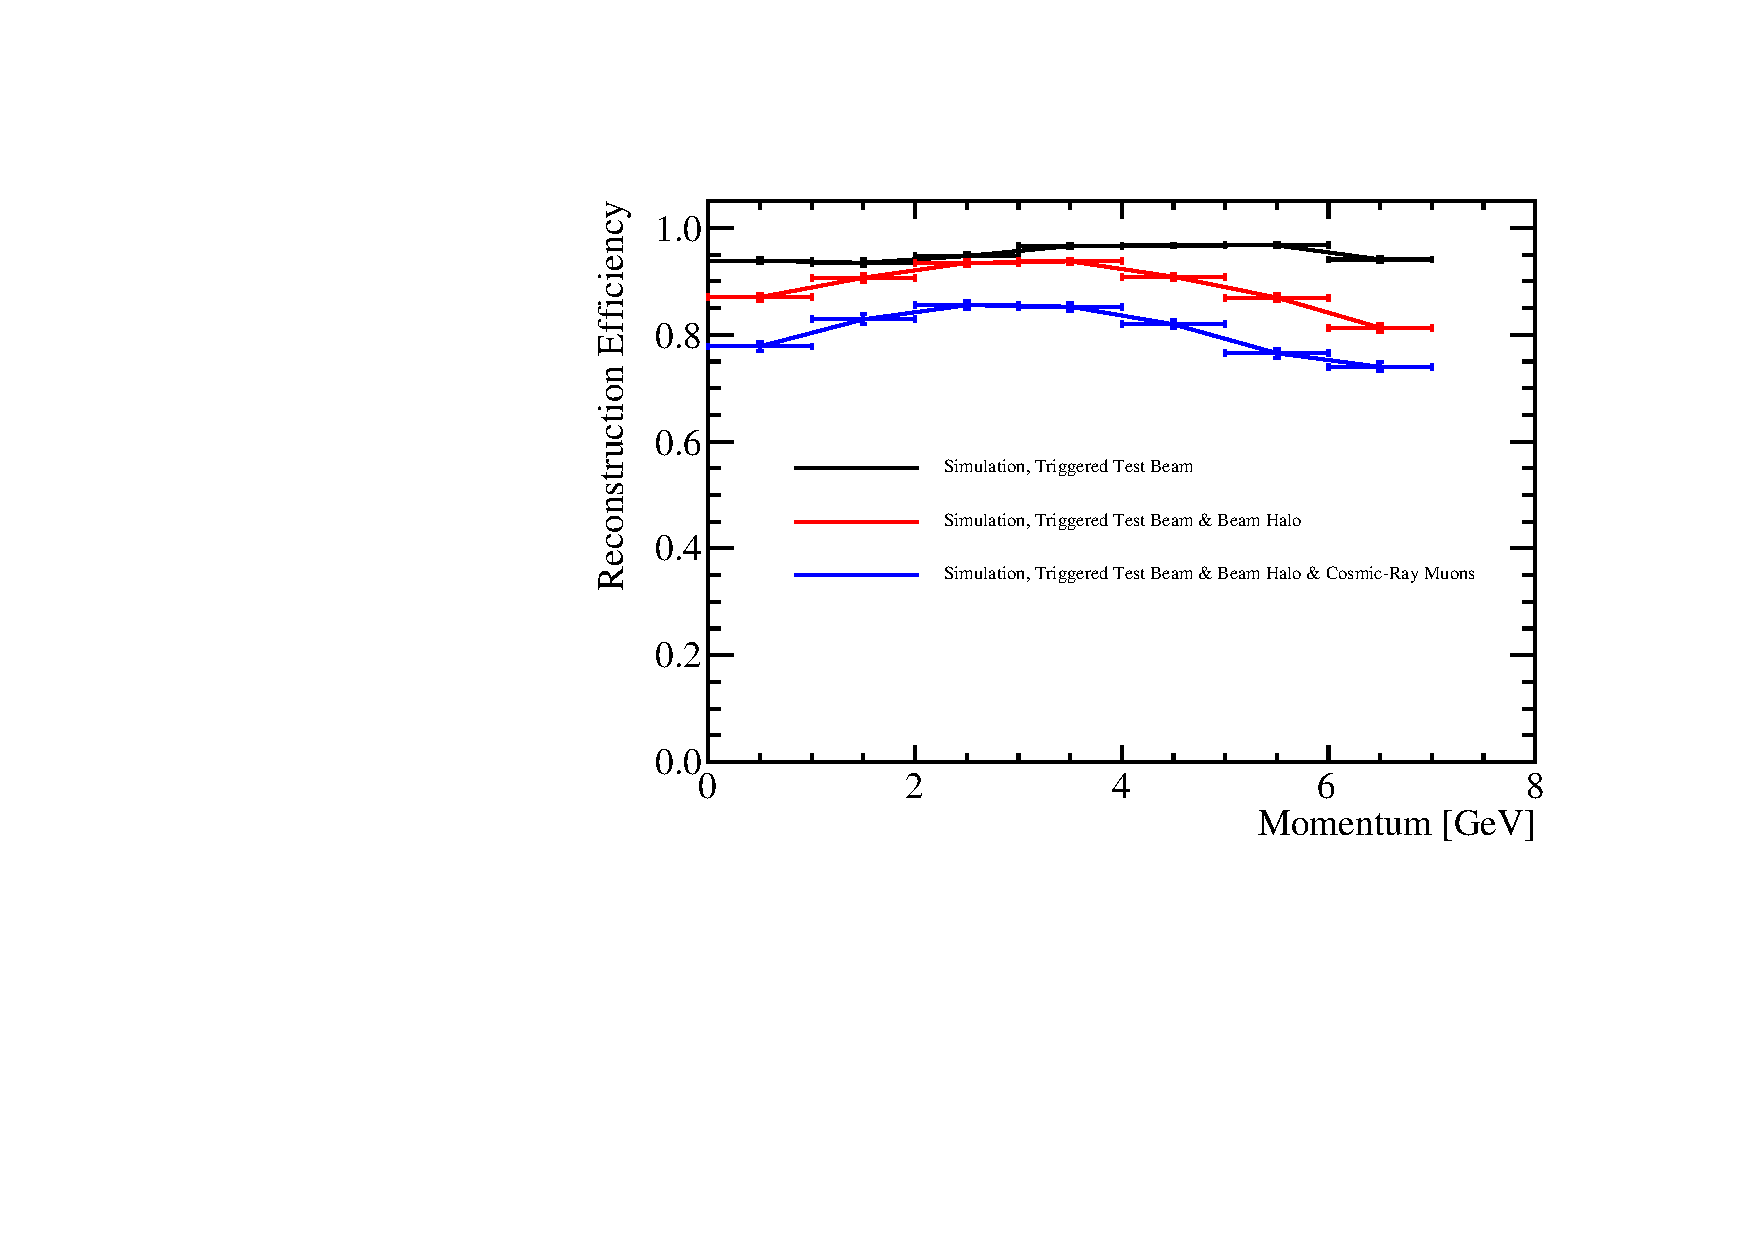
\includegraphics[width=0.45\textwidth]{Figures/Metrics/MC/Beam/Breakdown/BeamParticleEfficiencyVsMomentum.pdf}\label{fig:tbrecoeffbrkdwnp}} \\
\subfloat[]{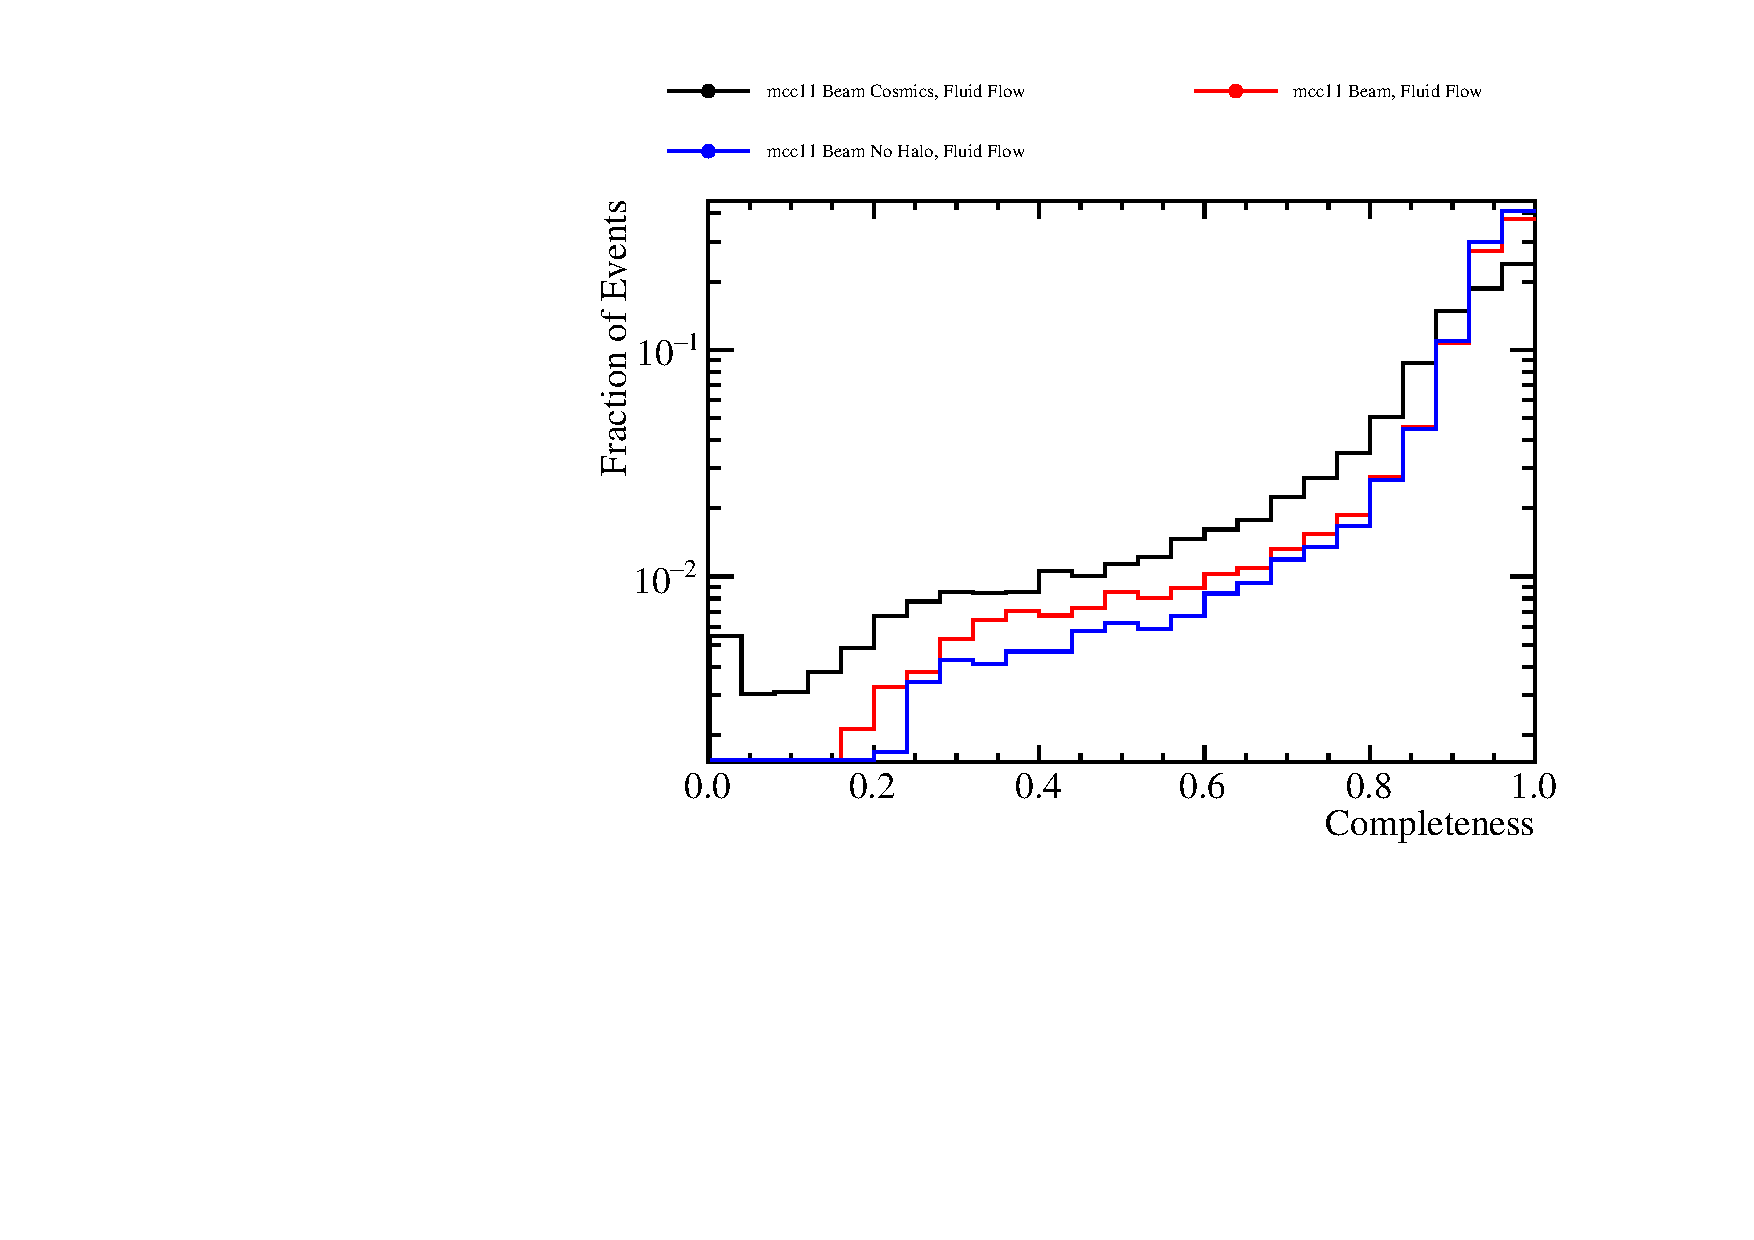
\includegraphics[width=0.45\textwidth]{Figures/Metrics/MC/Beam/Breakdown/BeamParticleCompleteness.pdf}\label{fig:tbrecoeffbrkdwncomp}}
\subfloat[]{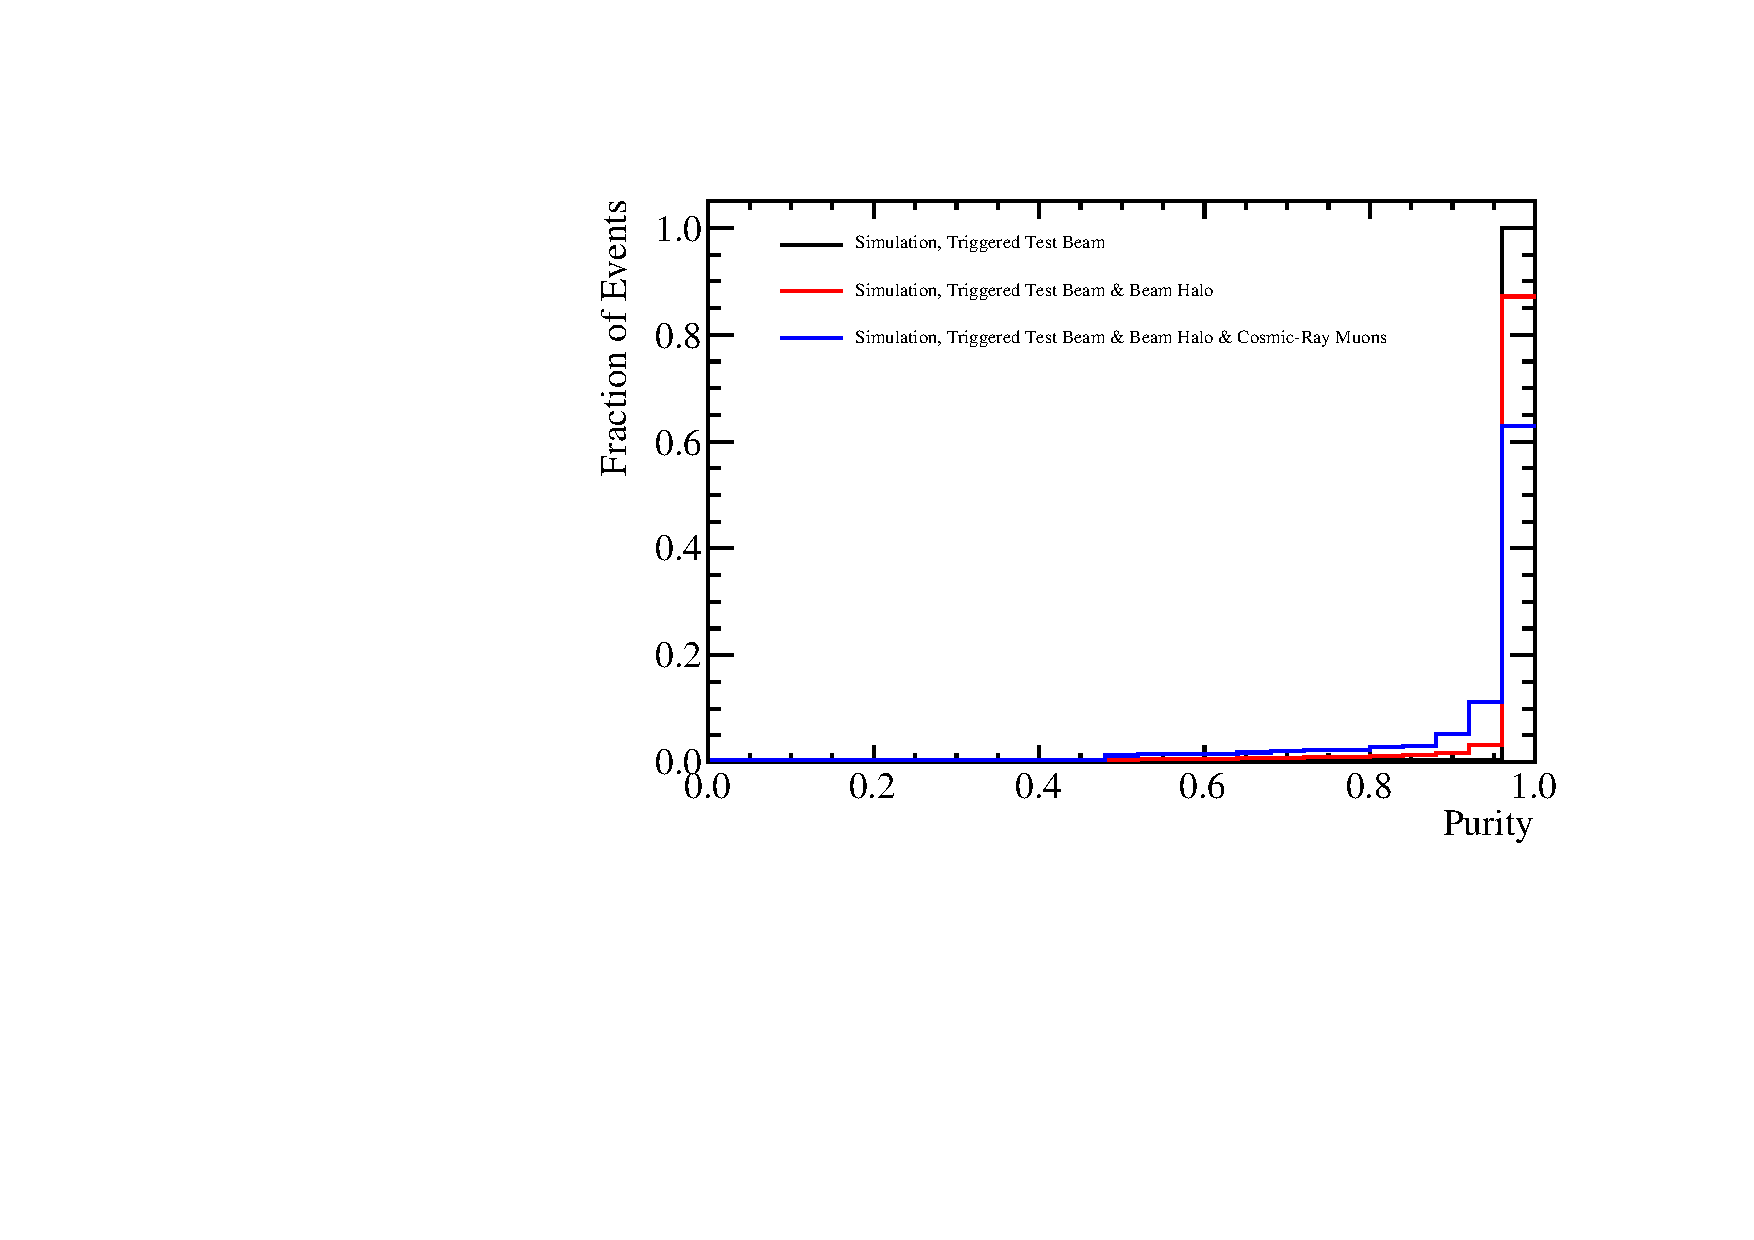
\includegraphics[width=0.45\textwidth]{Figures/Metrics/MC/Beam/Breakdown/BeamParticlePurity.pdf}\label{fig:tbrecoeffbrkdwnpur}}
\caption{The test beam particle reconstruction efficiency as a function of \protect\subref{fig:tbrecoeffbrkdwnnhits} the number of hits produced by the test beam particle and \protect\subref{fig:tbrecoeffbrkdwnp} the momentum of the test beam particle in simulation.  The error bars on the reconstruction efficiency show the statistical error.  Figures \protect\subref{fig:tbrecoeffbrkdwncomp} and \protect\subref{fig:tbrecoeffbrkdwnpur} show the completeness and purity of the reconstructed test beam particle.  These figures demonstrate the performance of the Pandora reconstruction in the nominal ProtoDUNE-SP environment (blue), the behaviour when the cosmic-ray muon background is removed (red) and the behaviour when both the cosmic-ray muon and the beam halo backgrounds are removed (black).}
\label{fig:tbrecoeffbrkdwn}
\end{figure}

\begin{figure}
\centering
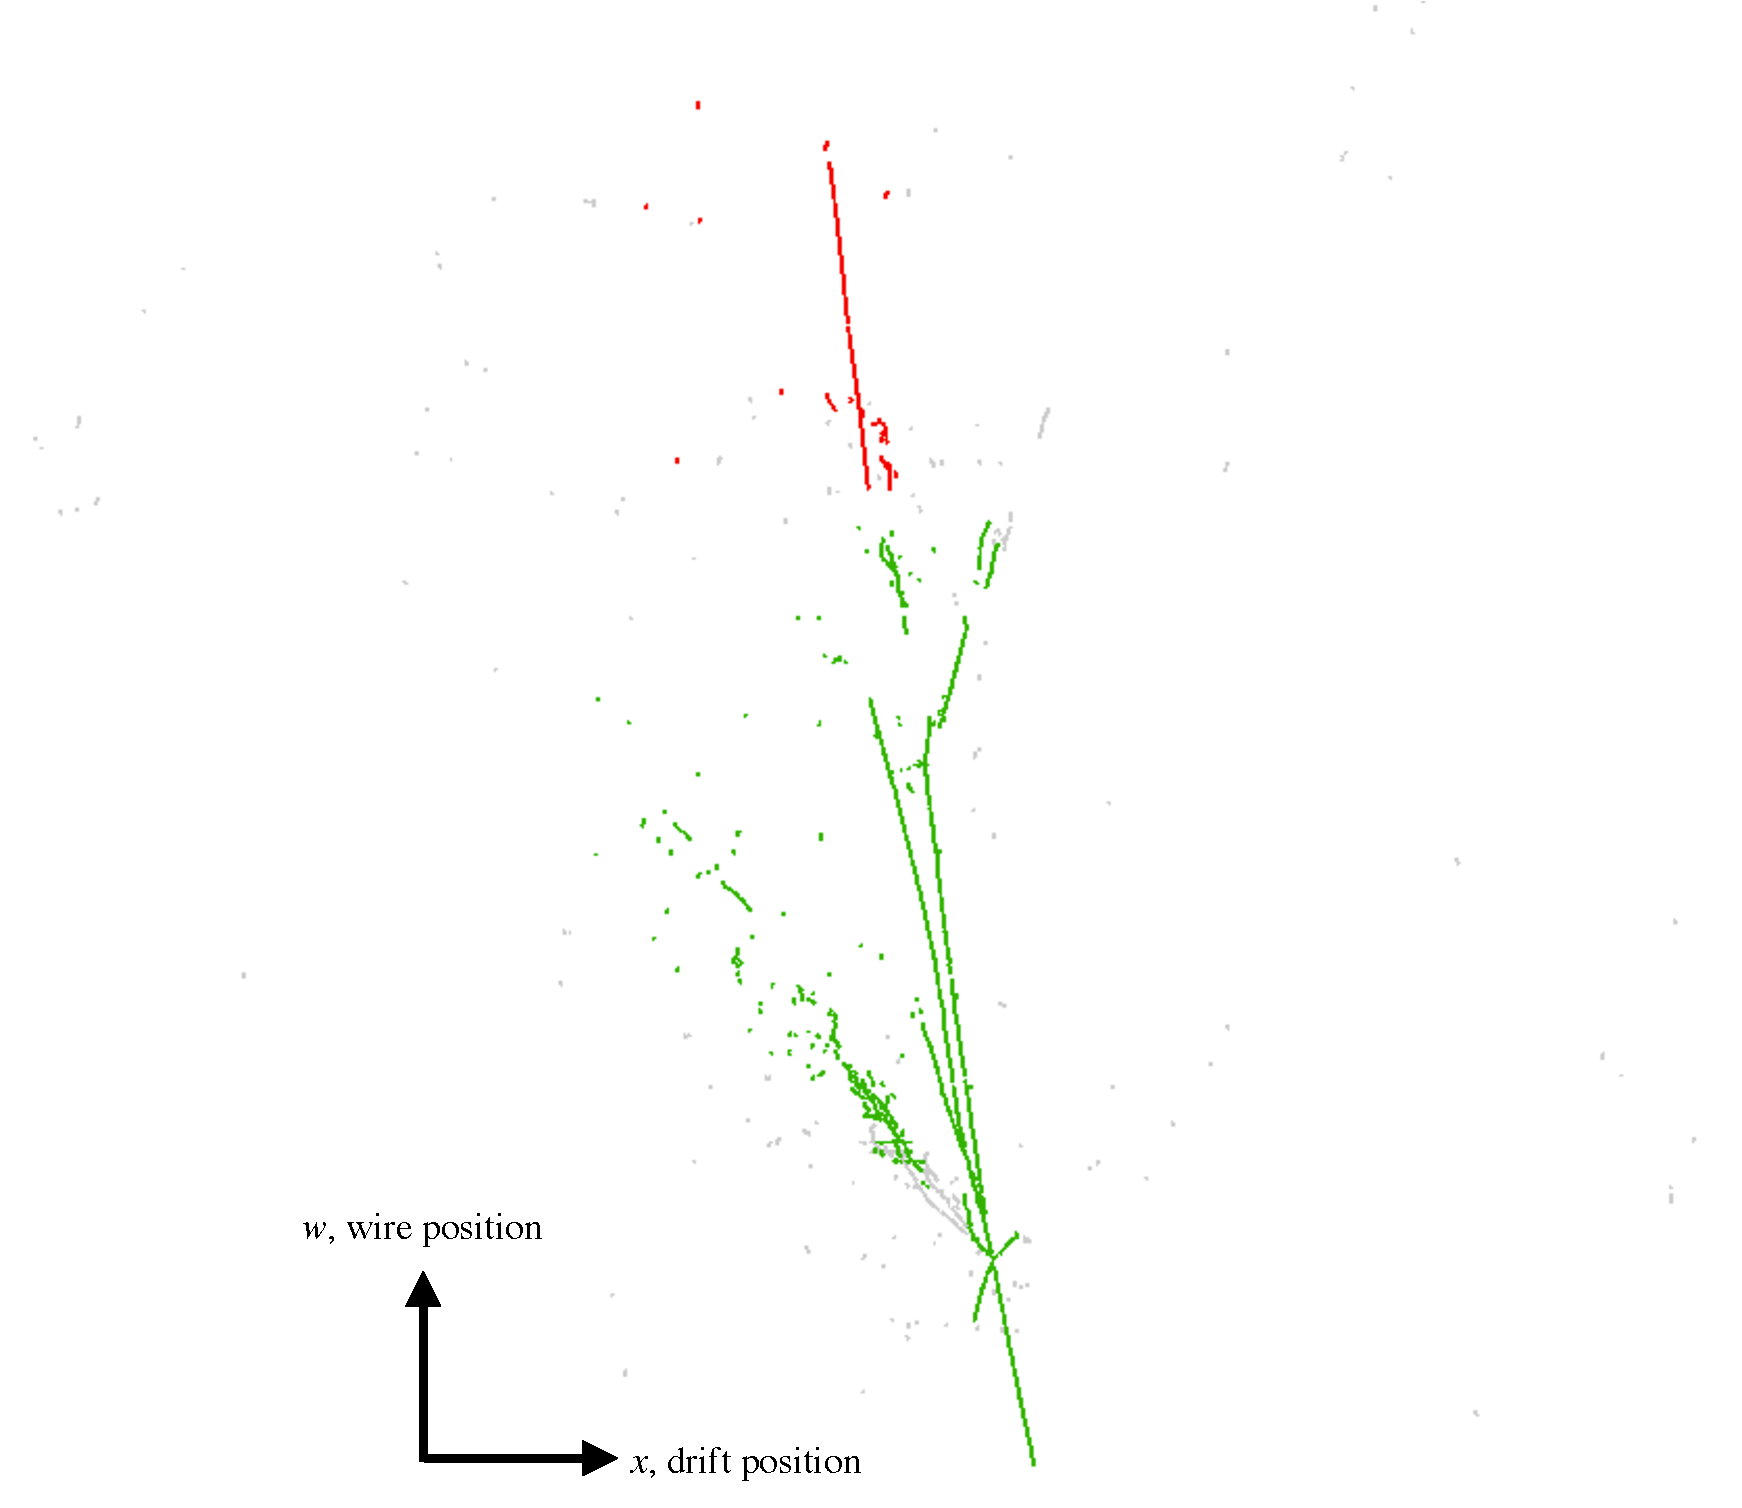
\includegraphics[width=0.5\textwidth]{Figures/EventDisplays/MC/CompletenessFigure.pdf}
\caption{An example of the $w$ view for a simulated 7~GeV $\pi^{+}$ event at ProtoDUNE-SP where the hits have been coloured to indicate the reconstructed particle they belong to; triggered beam particle (green) and cosmic-ray muon (red).  The remaining hits (grey) are diffuse hits that do not pass the reconstructable criteria.  This event contains only hits that originate from the triggered test beam particle and so serves as an example of how particles can be split up by the reconstruction leading a completeness of less than one.}
\label{fig:completenessfig}
\end{figure}

\begin{table}
\centering
\caption{The reconstruction efficiency for the test beam particle in ProtoDUNE-SP simulation as a function of beam momenta.}
\label{tab:1} 
\begin{tabular}{cc}
\hline\noalign{\smallskip}
Beam Momenta [GeV] & Reconstructed Efficiency  \\
\noalign{\smallskip}\hline\noalign{\smallskip}
1 & 87.5$\pm$0.8 \\
2 & 91.0$\pm$0.7 \\
3 & 92.7$\pm$0.6 \\
4 & 89.8$\pm$0.5 \\
5 & 89.0$\pm$0.5 \\
6 & 82.1$\pm$0.7 \\
7 & 75.4$\pm$0.7 \\
\noalign{\smallskip}\hline
\end{tabular}
\end{table}

\subsubsection{Cosmic-Ray Muon Reconstruction Metrics}
\label{sec:crmetrics}
Figure \ref{fig:crrecoeff} shows the reconstruction efficiency for cosmic-ray muons as a function of the number of hits in the detector, which yields an integrated efficiency of 95\%.  The purity and completeness of the reconstructed cosmic-ray muons are shown in figure \ref{fig:crrecopurcom}, both of which show strong peaks at one.

\begin{figure}
\centering
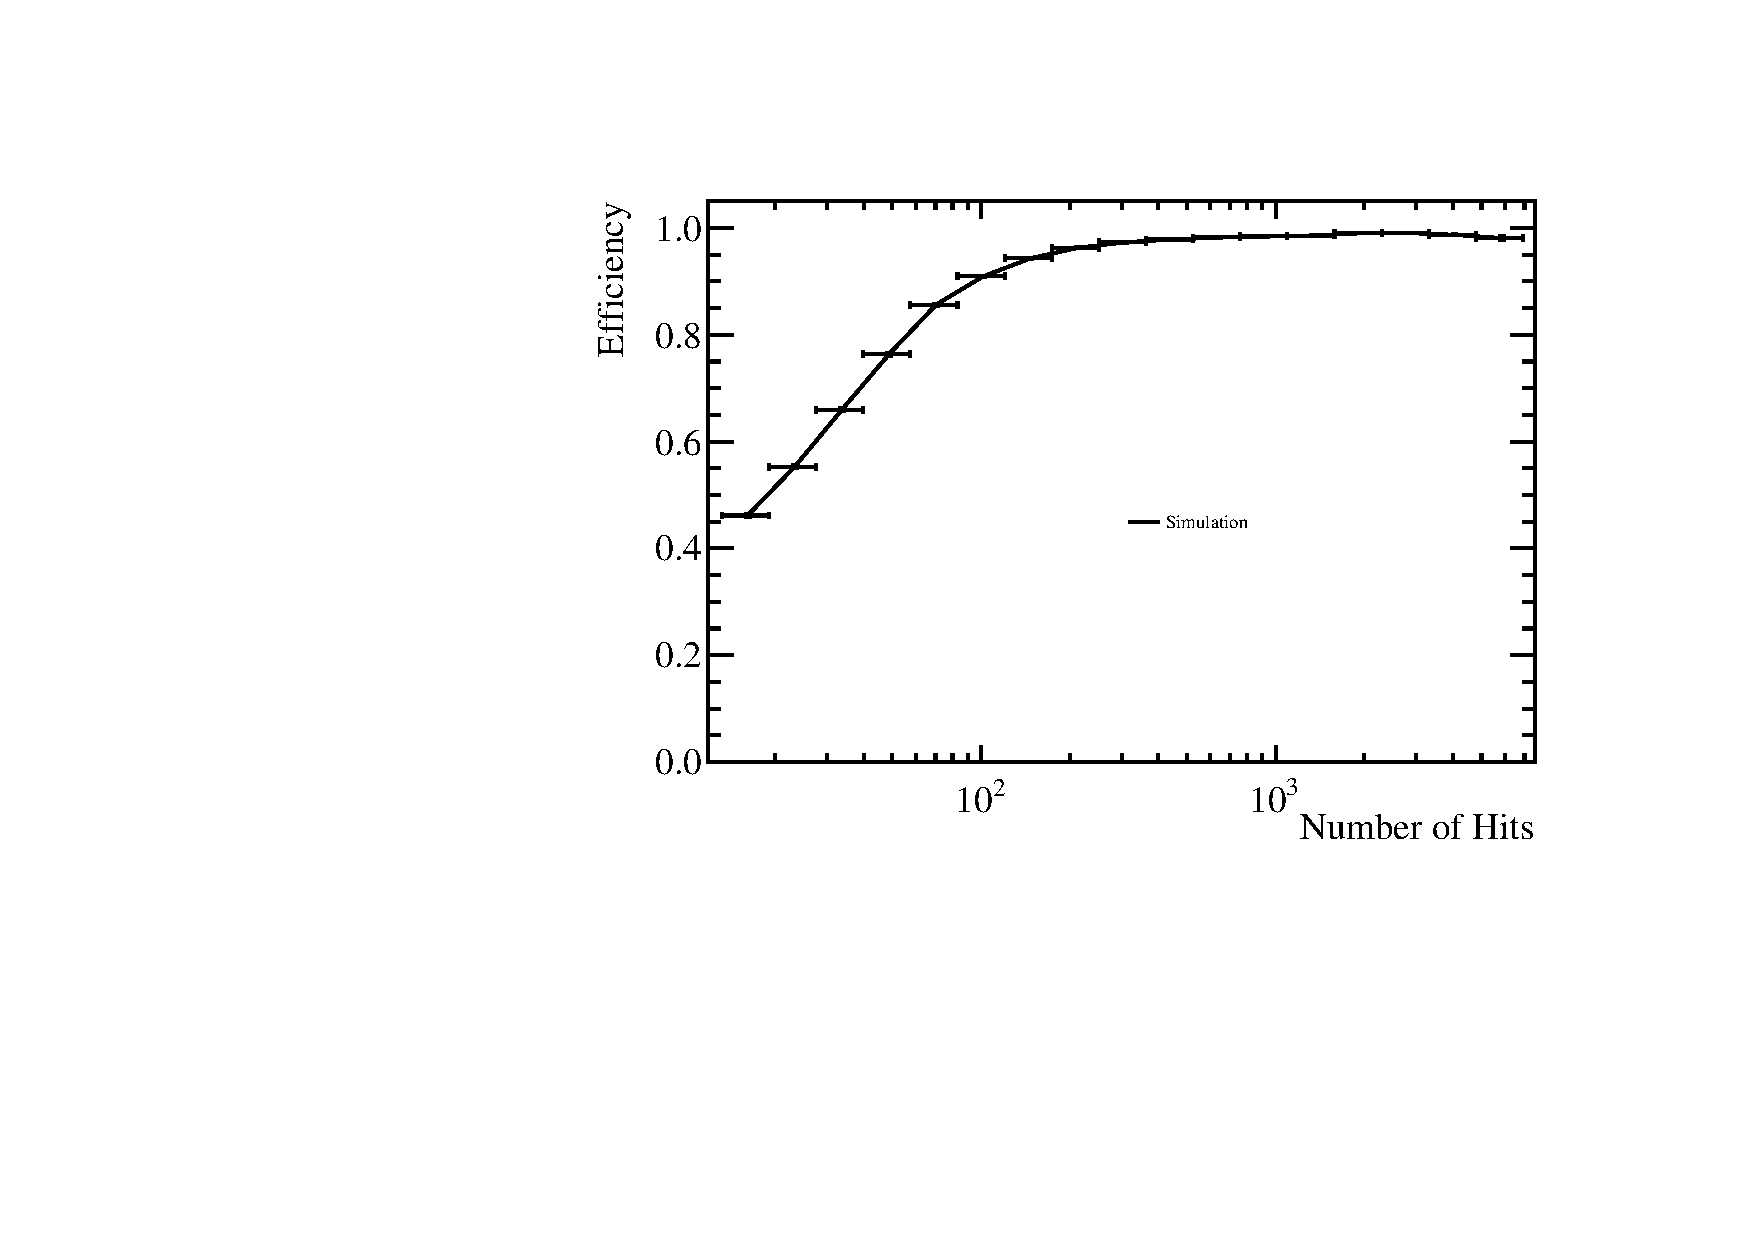
\includegraphics[width=0.75\textwidth]{Figures/Metrics/MC/Cosmics/CosmicRayEfficiencyVsNHits.pdf}
\caption{The reconstruction efficiency for cosmic-ray muons in ProtoDUNE-SP simulation as a function of number of hits.}
\label{fig:crrecoeff}
\end{figure}

\begin{figure}
\subfloat[]{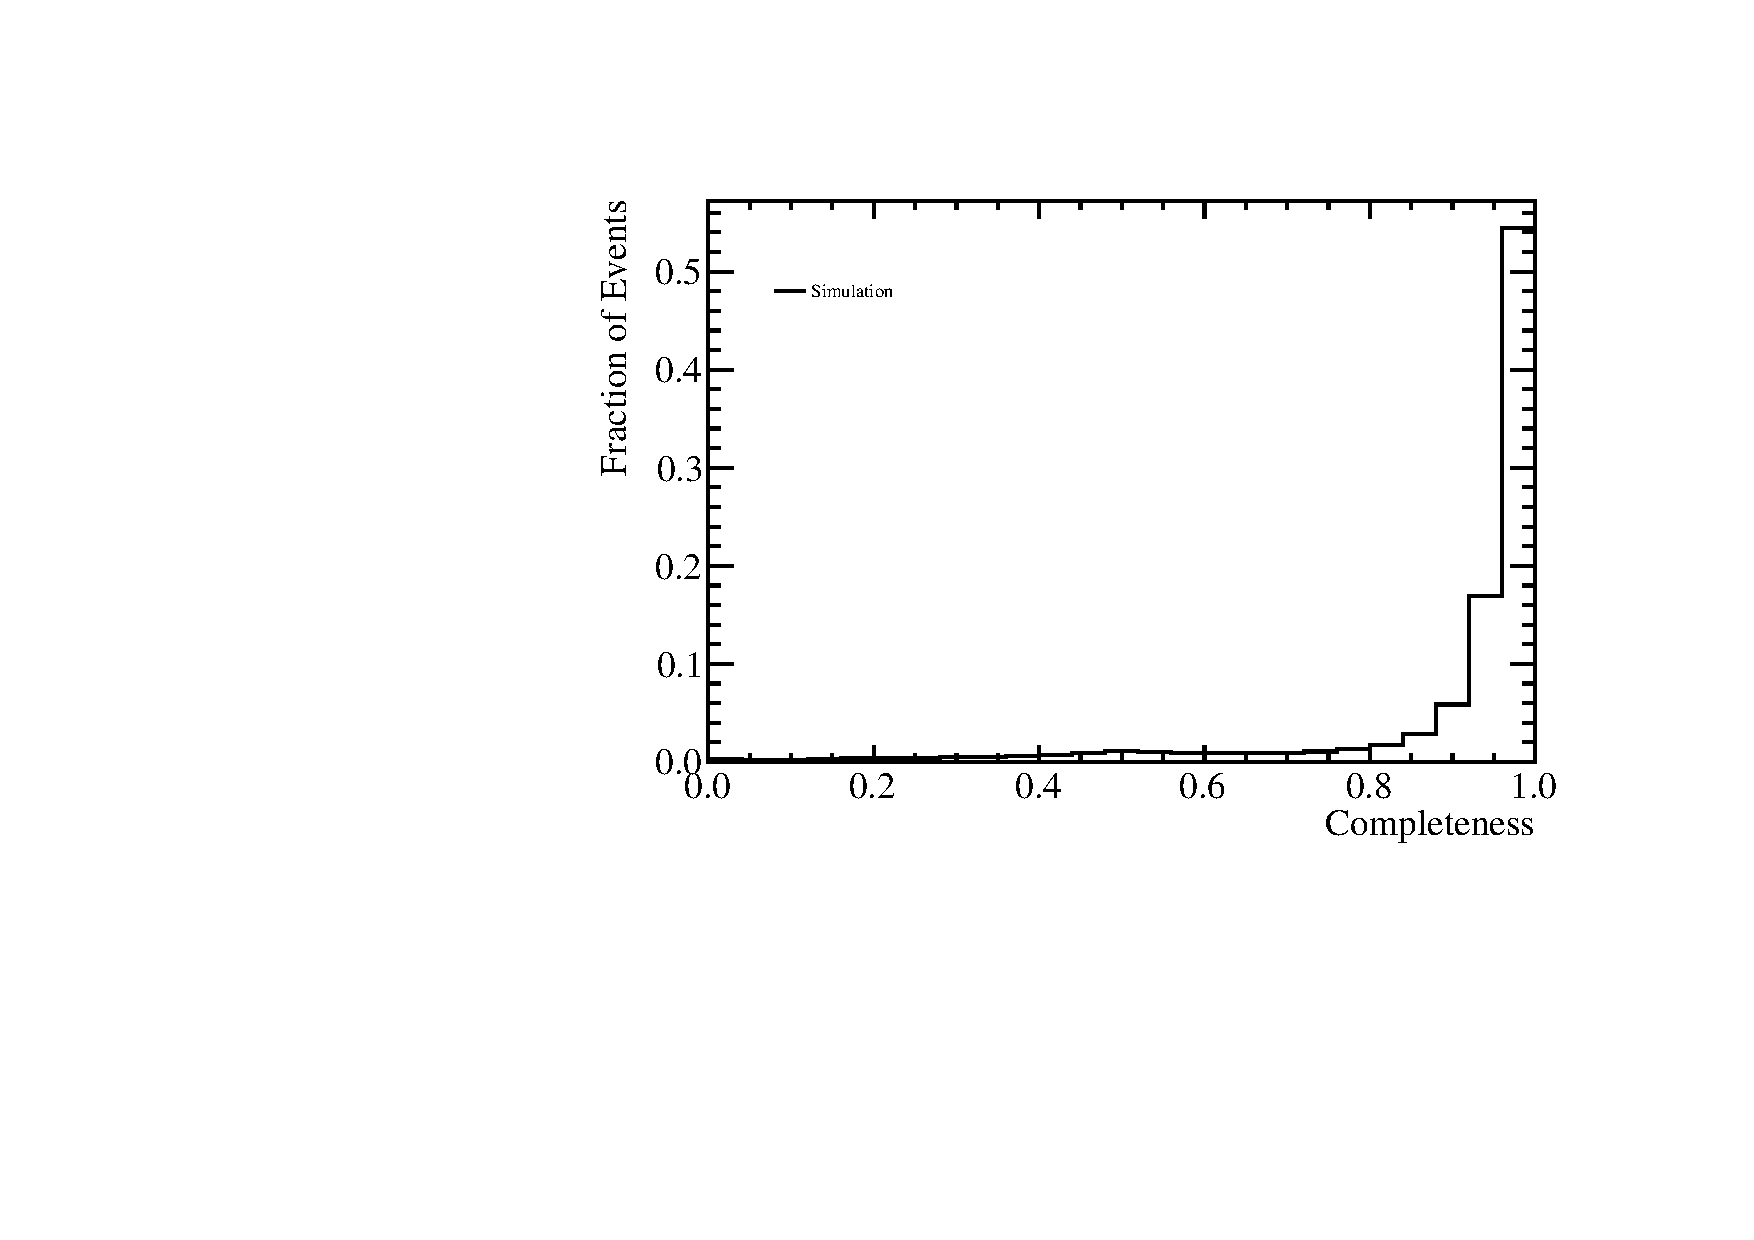
\includegraphics[width=0.5\textwidth]{Figures/Metrics/MC/Cosmics/CosmicRayCompleteness.pdf}\label{fig:crrecocom}}
\subfloat[]{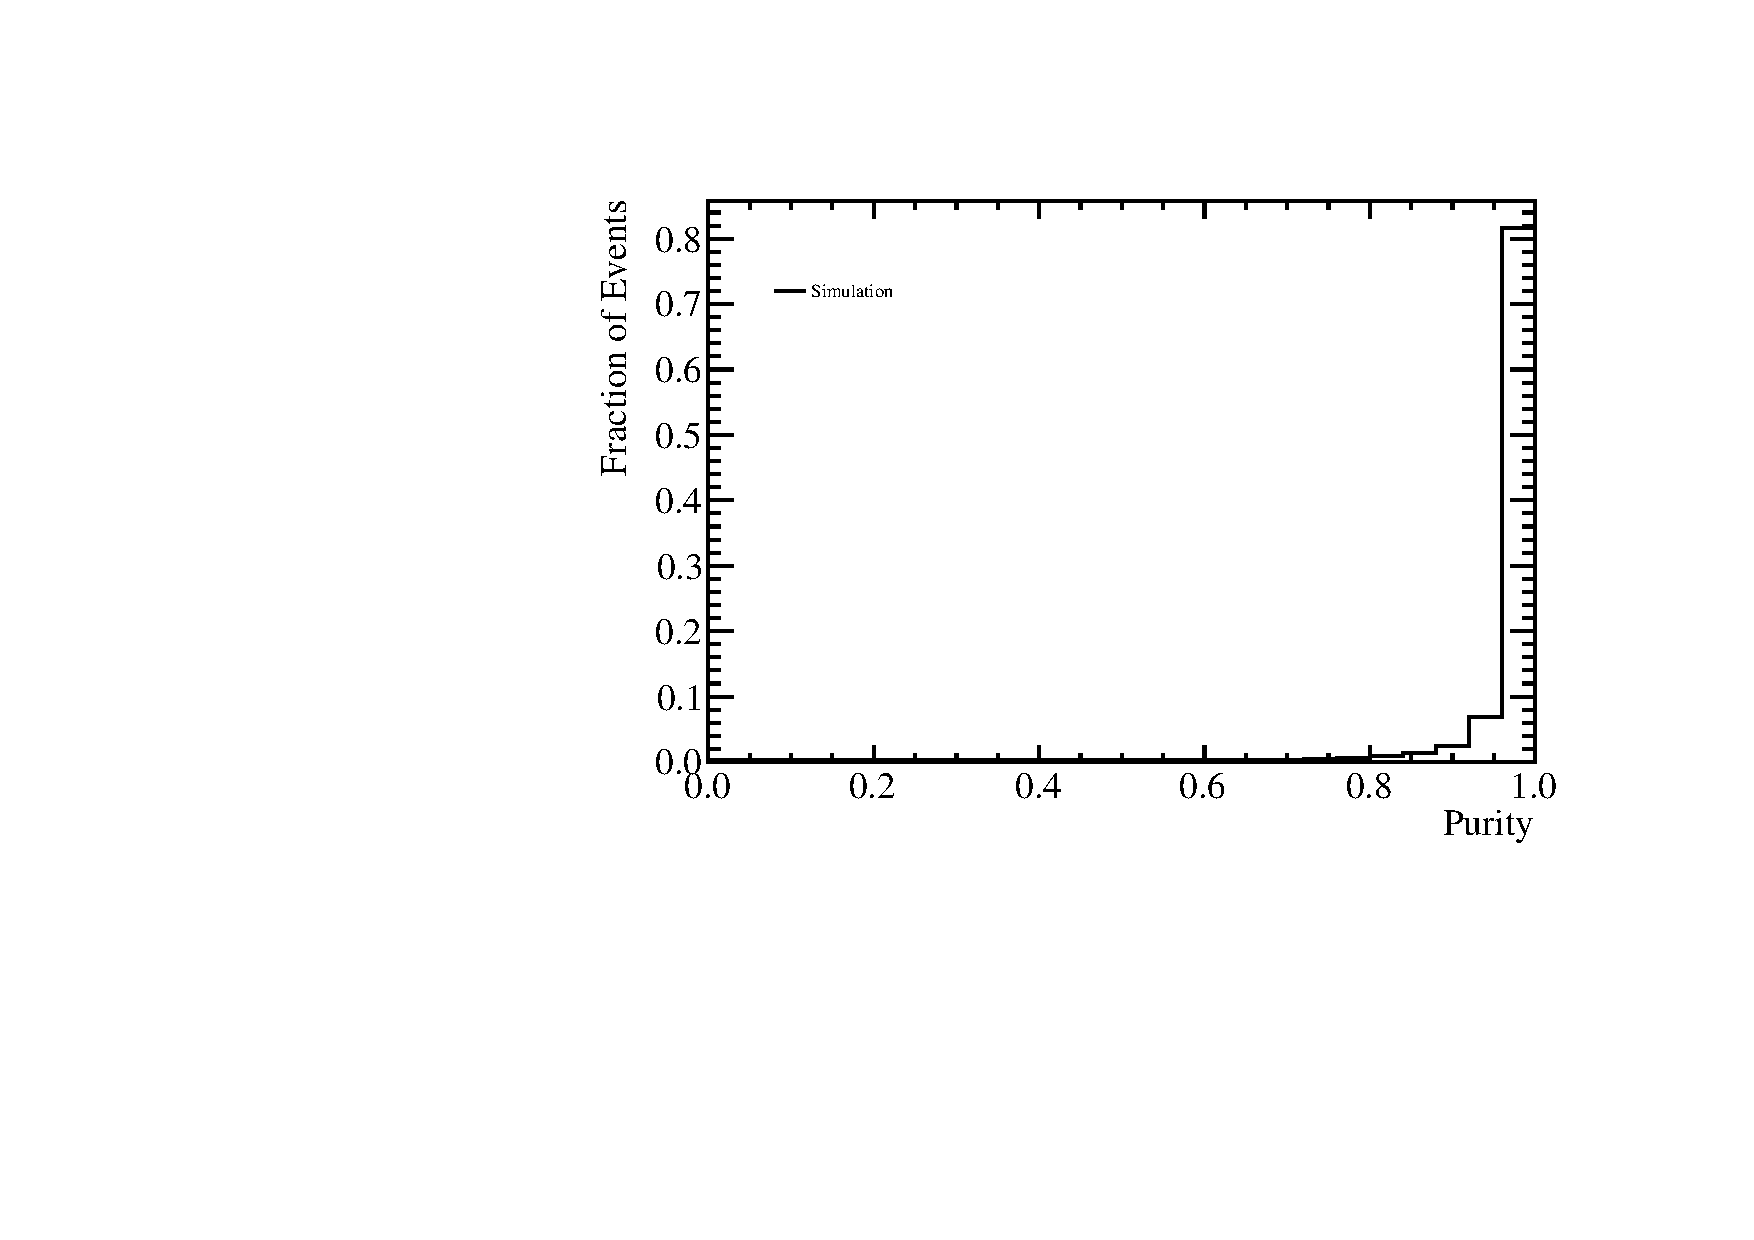
\includegraphics[width=0.5\textwidth]{Figures/Metrics/MC/Cosmics/CosmicRayPurity.pdf}\label{fig:crrecopur}}
\caption{\protect\subref{fig:crrecocom} the completeness and \protect\subref{fig:crrecopur} purity of reconstructed cosmic-ray muon particles in simulation.}
\label{fig:crrecopurcom}
\end{figure}

It is also possible to tag the true $T_{0}$ of reconstructed cosmic-ray muons if they are stitched by the process discussed in section \ref{sec:consolidatedreco}.  The distribution of the resolution of the reconstructed $T_{0}$ for cosmic-ray muons is shown in figure \ref{fig:crt0res}.  As expected, the impact of space charge \todo{description and reference to space charge} in the simulation leads to a degradation in the $T_{0}$ resolution and the addition of the fluid flow model, which includes asymmetric space charge effects, leads to further degradation.  

\begin{figure}
\centering
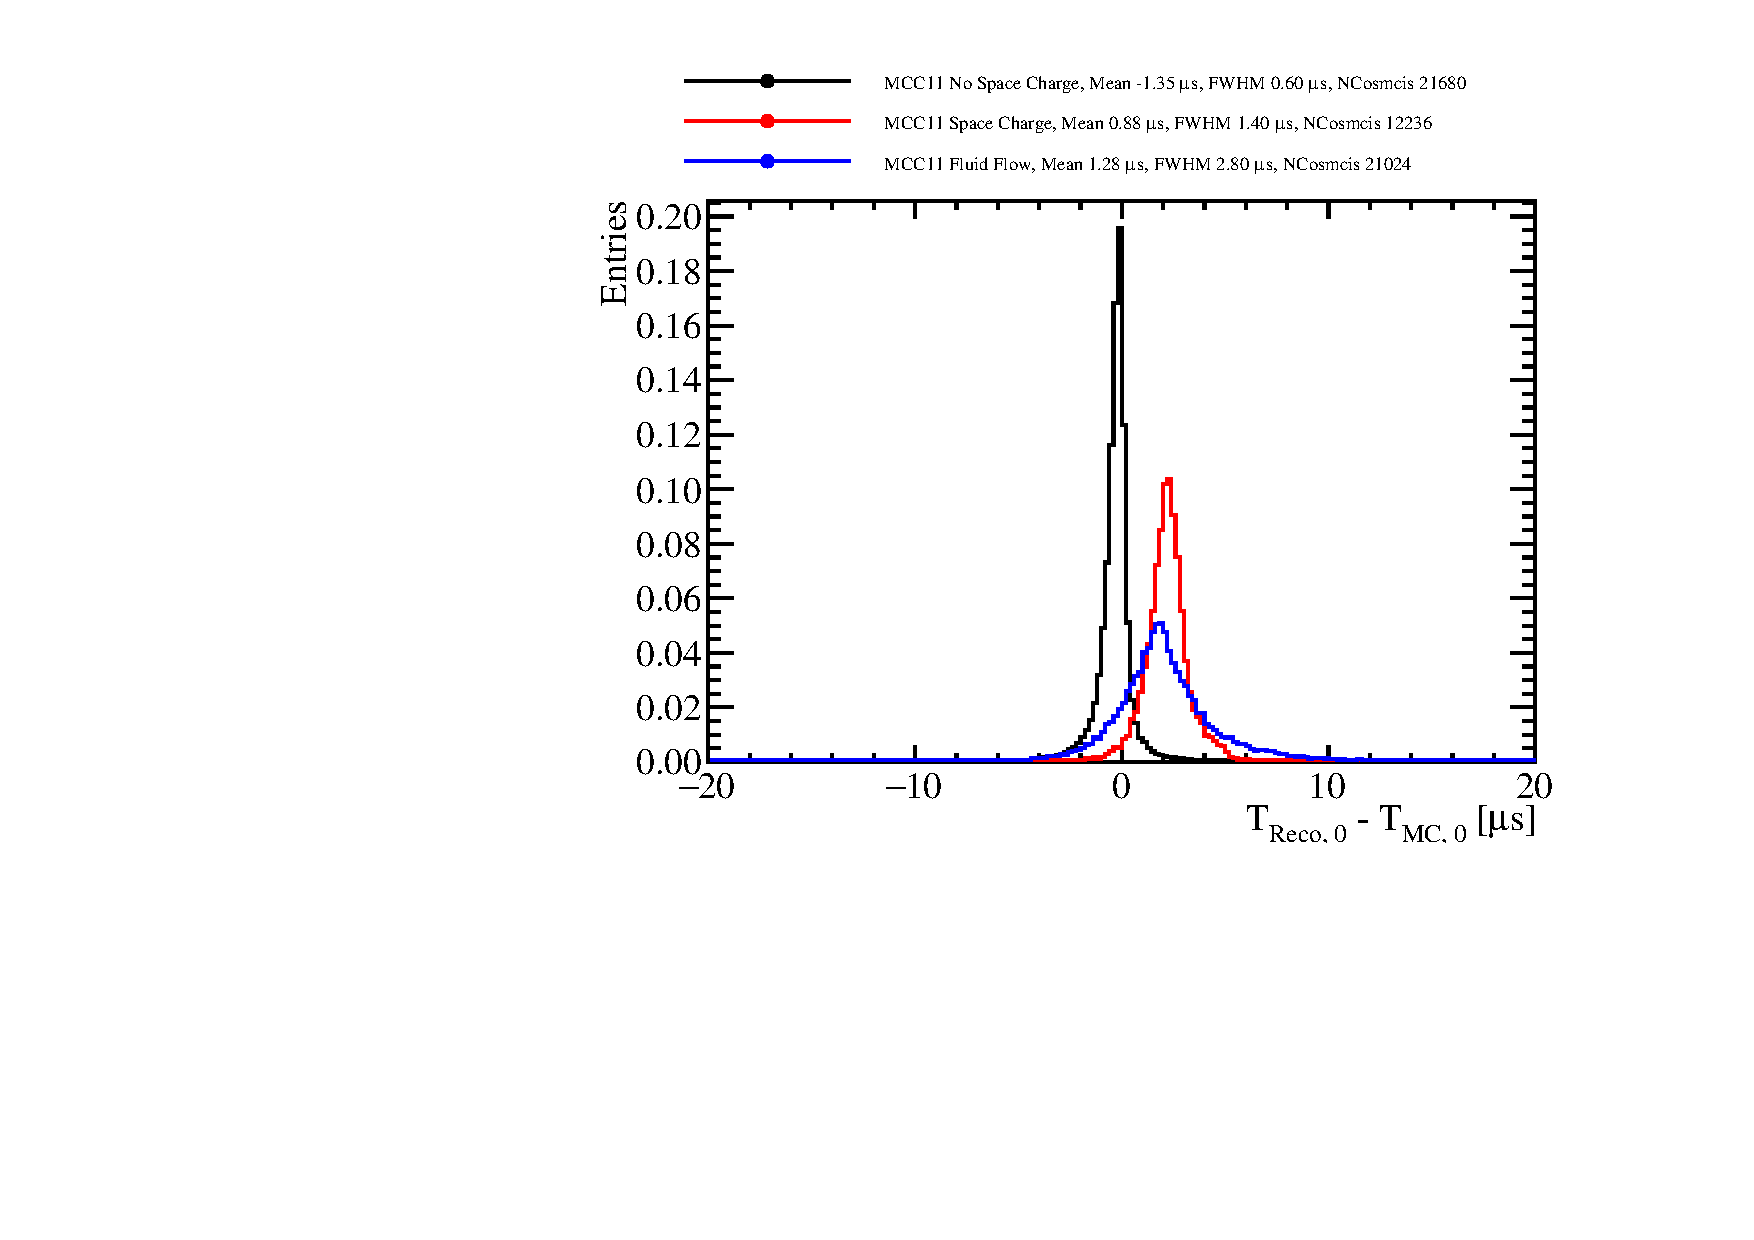
\includegraphics[width=0.75\textwidth]{Figures/Metrics/MC/Cosmics/CosmicRayT0Resolustion.pdf}
\caption{The resolution on the reconstructed $T_{0}$ for cosmic-ray muons in MC.}
\label{fig:crt0res}
\end{figure}

In order to give context to the topologies that the reconstruction is faced with at ProtoDUNE-SP an estimate of the number of cosmic-ray muons passing through the detector per event has been made.  The number of reconstructed cosmic-ray muons matched to clear cosmic-ray muons, i.e. depositing more than 100 hits in the detector, is shown as a function of the number of clear cosmic-ray muons in figure \ref{fig:crnperevt}.  This shows that, on a per event basis, the reconstruction is predominantly working on the reconstruction of cosmic-ray muons.

\begin{figure}
\centering
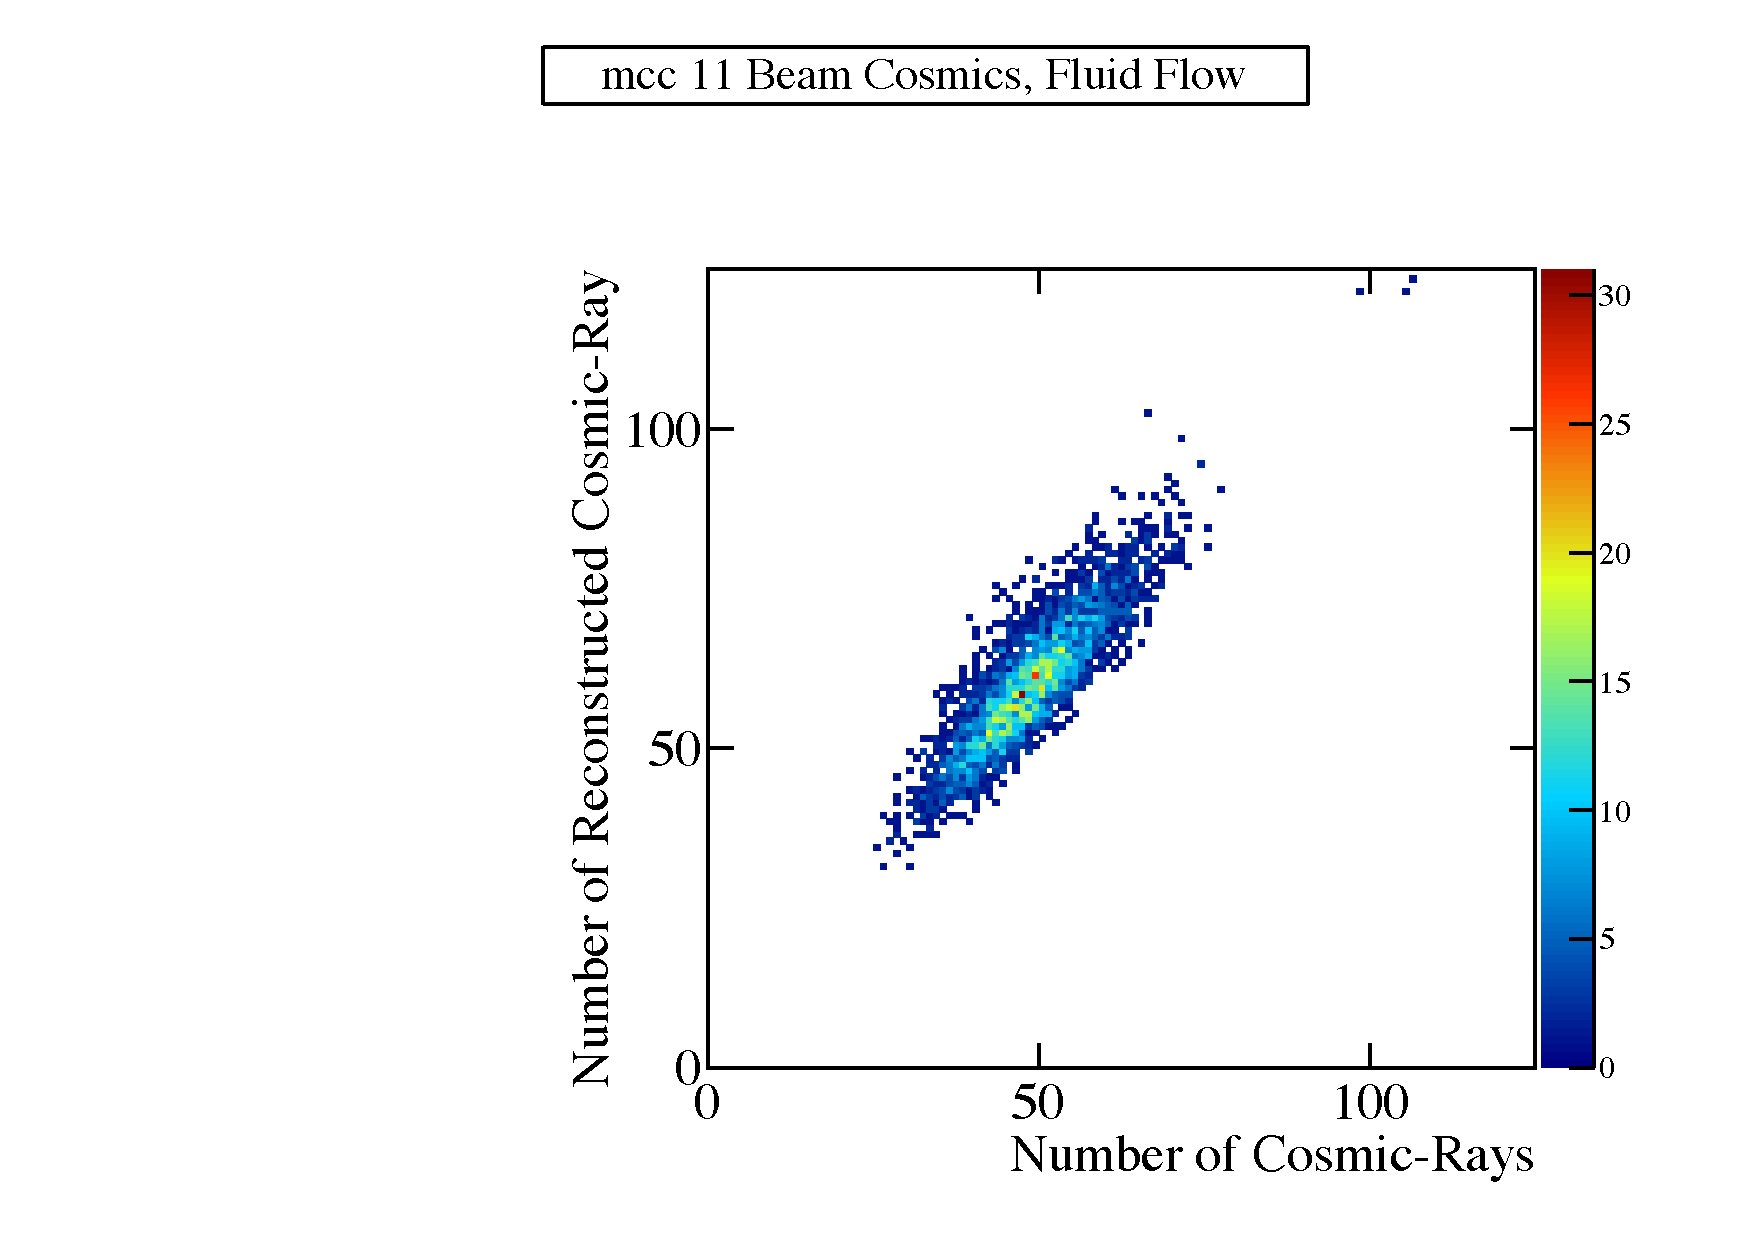
\includegraphics[width=0.75\textwidth]{Figures/Metrics/MC/Cosmics/CRMatchesCosmicRayEvent.pdf}
\caption{The number of matched reconstructed cosmic-ray muons per event as a function of the true number of cosmic-ray muons for cosmic-ray muons depositing more than 100 hits in the detector.  The cut at 100 hits allows a clearer comparison to be made to data in subsequent studies due to the higher reconstruction efficiency for these cosmic-ray muons with respect to those depositing less than 100 hits.}
\label{fig:crnperevt}
\end{figure}

\subsection{Data}

ProtoDUNE-SP took test beam data at CERN between October and December 2018.  What follows is a flavour of how the Monte-Carlo metrics discussed above compare to data.  This data presents the Pandora reconstruction with several unique challenges that have not been seen at other active LArTPC experiments, such as stitching of cosmic-ray muons due to the presence of multiple drift volumes and the reconstruction of test beam particle interactions as opposed to neutrino interactions.  

\subsubsection{Test Beam Metrics}
A crucial metric describing the performance of the pattern recognition at ProtoDUNE-SP is the triggered test beam particle reconstruction efficiency.  This metric folds in effects from each step of the reconstruction procedure and crucially the test beam particle id step.  In order for a reconstructed event to be counted as efficient, a reconstructed object must be classified as originating from the test beam.  As access to the underlying truth information for data is not possible, the reconstruction metric used for this data MC comparison does not use the matching procedure described in section \ref{sec:mcmetrics}.  Instead an event is deemed efficient when for:

\begin{itemize}
    \item \textbf{Data} The trigger is active and indicates the presence of a single particle and there is a reconstructed test beam particle in the event output.
    \item \textbf{Monte-Carlo} There is a triggered test beam particle in the MC particle hierarchy and there is a reconstructed test beam particle in the event output.
\end{itemize}

The reconstruction efficiency for ProtoDUNE for separate beam momentum runs is shown in table \ref{tab:dataeff}.  

\begin{table}
\centering
\caption{The reconstruction efficiency for test beam particle interactions in data as a function of beam momenta for ProtoDUNE-SP.}
\label{tab:dataeff} 
\begin{tabular}{cc}
\hline\noalign{\smallskip}
Beam Momenta [GeV] & Reconstructed Efficiency  \\
\noalign{\smallskip}\hline\noalign{\smallskip}
1 & 70.6$\pm$0.3 \\
2 & 84.2$\pm$0.3 \\
3 & 86.8$\pm$0.2 \\
6 & 85.2$\pm$0.2 \\
7 & 83.7$\pm$0.2 \\
\noalign{\smallskip}\hline
\end{tabular}
\end{table}

The ProtoDUNE trigger also measures the momentum of the triggered test beam particle, therefore the reconstruction efficiency is plotted as a function of the triggered test beam particle momentum in figure \ref{fig:datamcrecoeff}.  

\begin{figure}
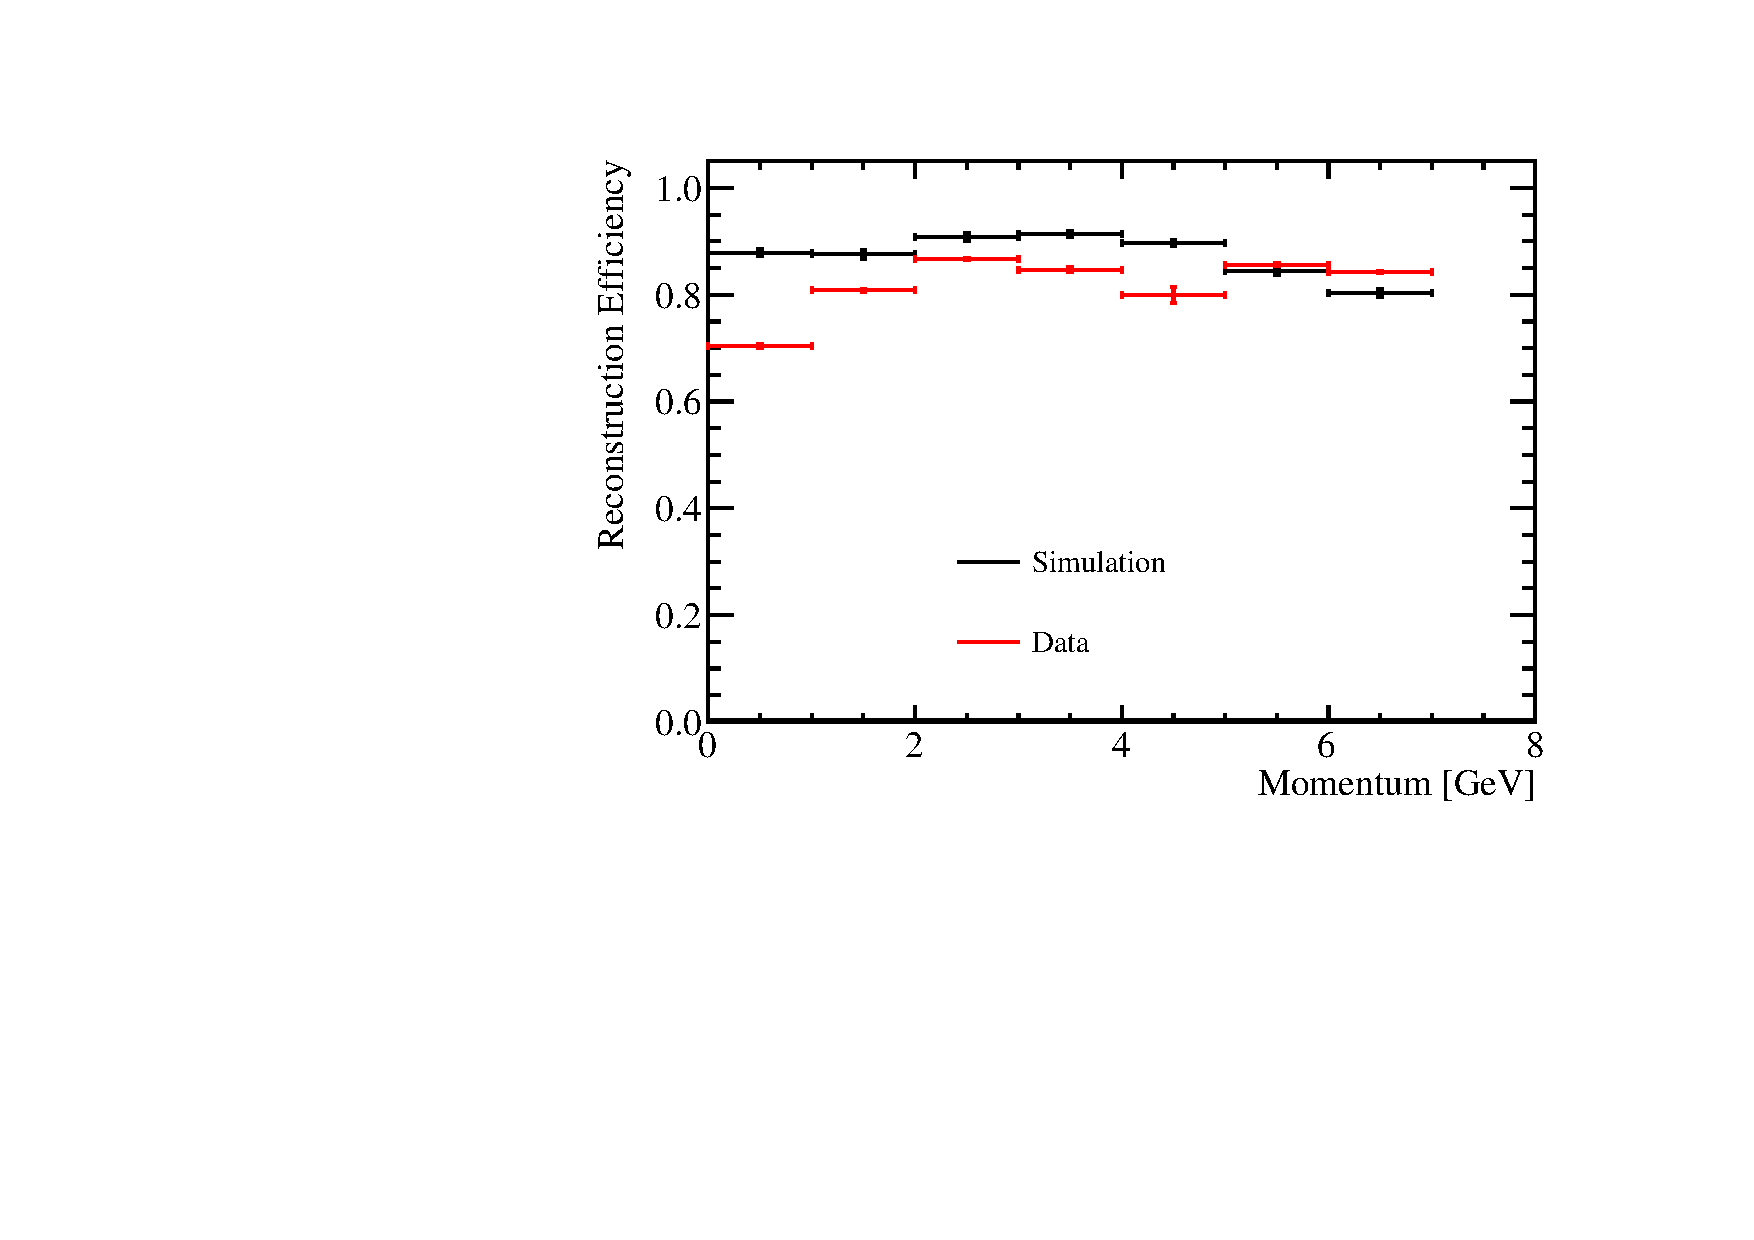
\includegraphics[width=1.0\textwidth]{Figures/Metrics/Data/Beam/BeamParticleEfficiencyVsMomentum.pdf}
\caption{The test beam particle reconstruction efficiency as a function of the number of hits in the test beam particle and the test beam particle momentum.}
\label{fig:datamcrecoeff}
\end{figure}

Overall, there is a typically good agreement between the reconstruction efficiency for data and MC with integrated efficiencies of ~80\% and ~80\% respectively.  As a function of momentum, additional features are present.  In particular, at low momentum, where the reconstruction efficiency for data is lower than MC, and high momentum, where the reconstruction efficiency is higher for data than MC.  The disparity at low momenta is due to the trigger being active for certain events, but no clear test beam particle appearing in the detector. \todo{Expect request for justification}  For high momenta, the disparity is due to an overestimation of the beam halo in the MC samples.  This is evident from figure \ref{fig:tbrecoeffbrkdwn}, which indicates that the impact of cosmic-ray muons at high beam momenta is almost negligible, while the beam halo dominates in inefficiencies in the reconstruction efficiency.  

In addition to the reconstruction efficiency it is also possible to evaluate higher level metrics for the reconstructed test beam particle describing the quality of the reconstructed object.  For example figure \ref{fig:openingangles} shows the opening angle between the reconstructed and expected direction of the triggered test beam particle.  For data the trigger provides a measurement of the particle direction, while for MC truth information is used for comparison.  While differences are present it is encouraging that both of these distributions peak at low values of opening angle.  The same distributions divided into track and shower like triggered test beam particles are included.  The broader distribution for showers indicates that, as expected, estimation of the direction of a clean single track like 3D particle is more precise than the estimation of a more disperse shower like object.   

\begin{figure}
\subfloat[]{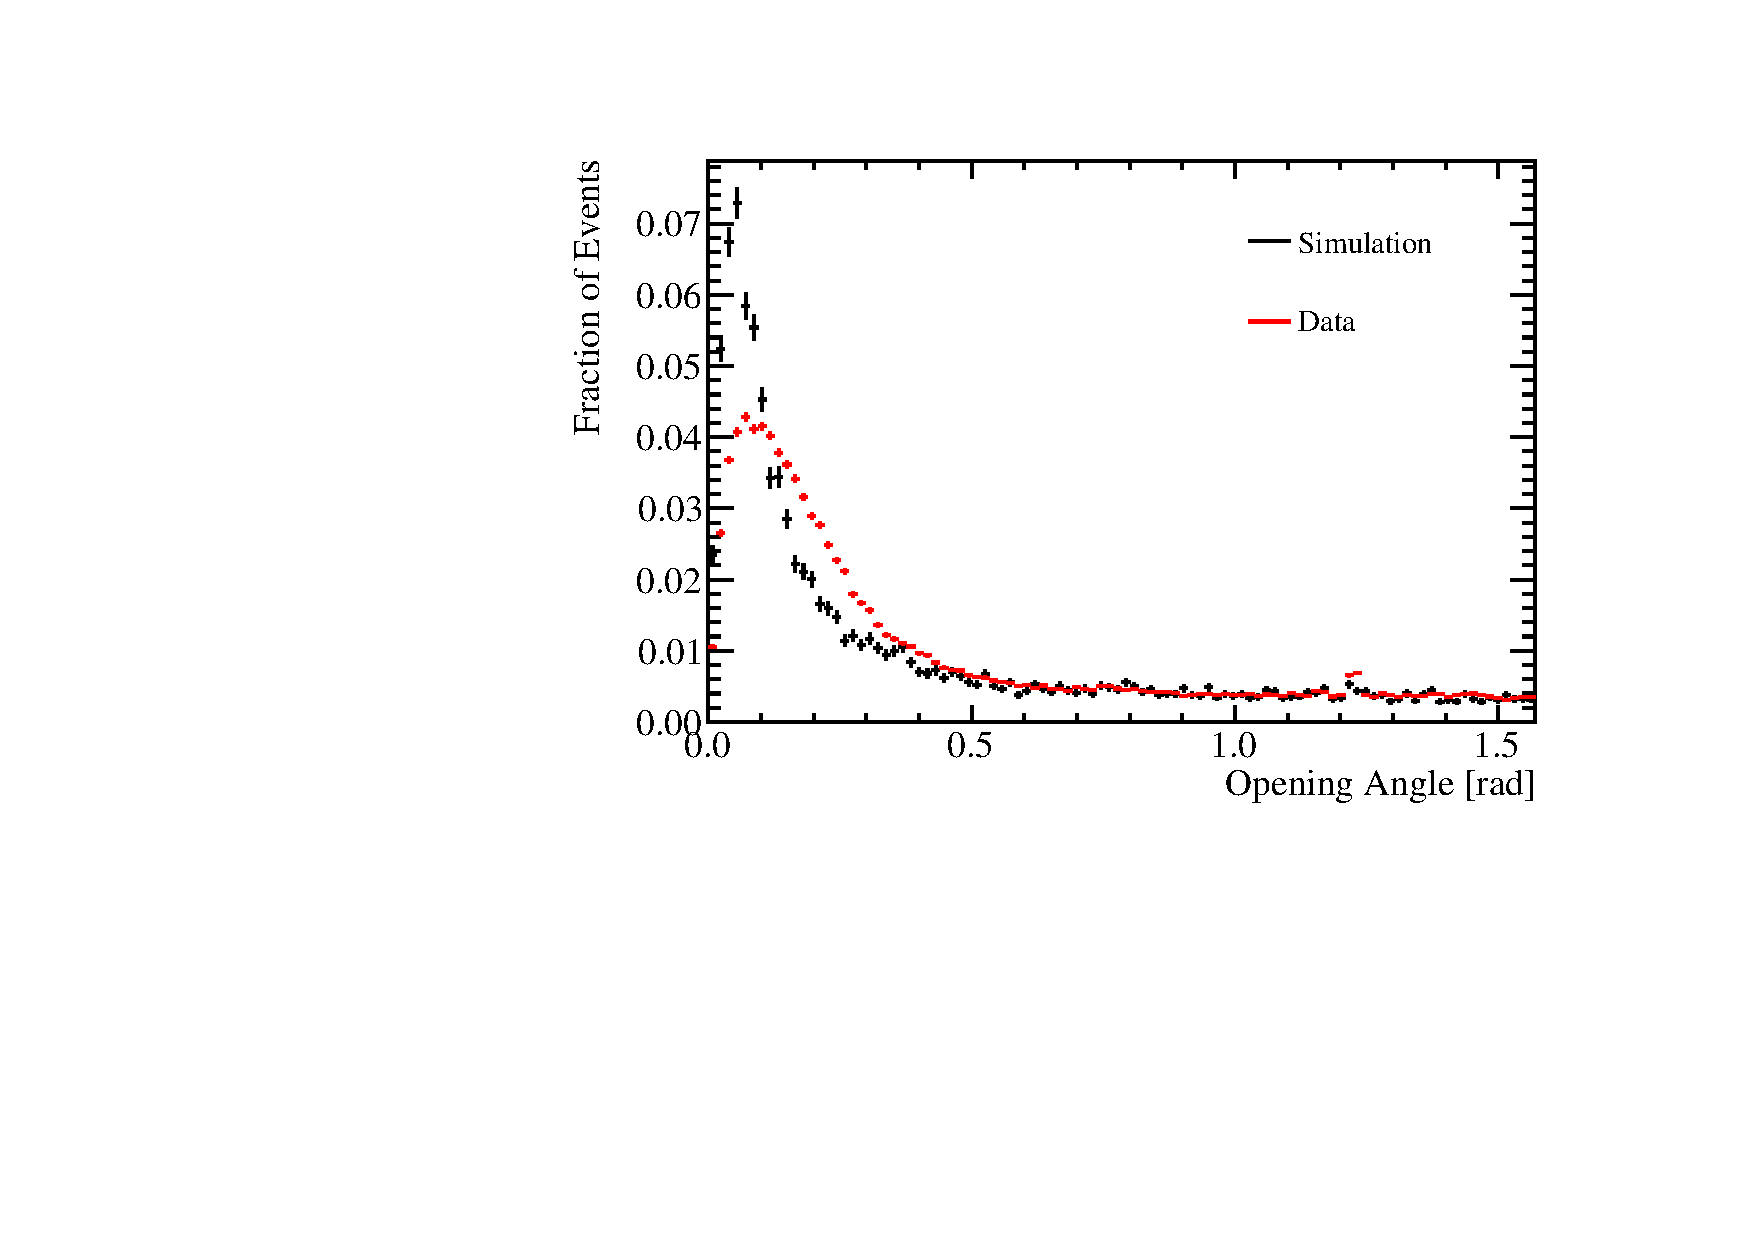
\includegraphics[width=1.0\textwidth]{Figures/Metrics/Data/Beam/BeamParticleOpeningAngle.pdf}\label{fig:openingangle}} \\
\subfloat[]{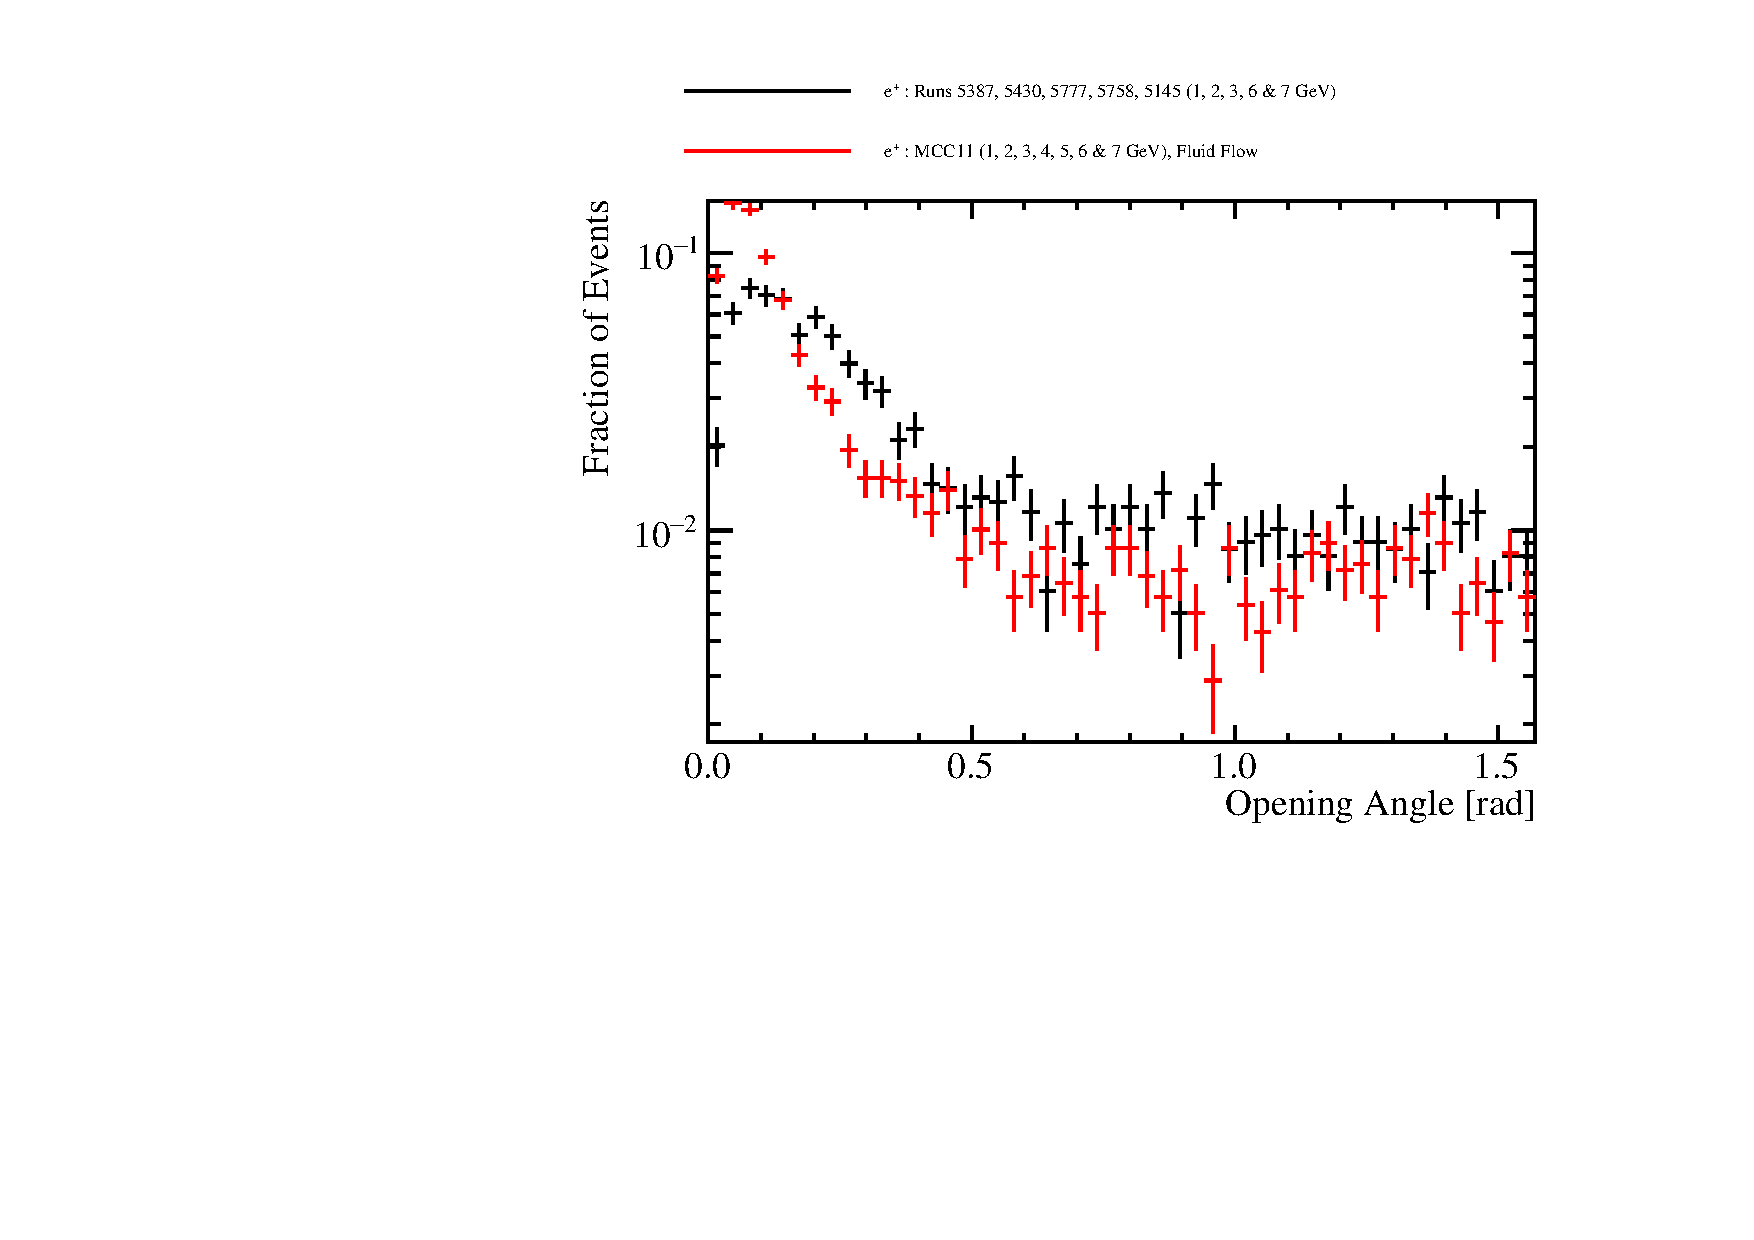
\includegraphics[width=0.5\textwidth]{Figures/Metrics/Data/Beam/BeamParticleOpeningAngleElectron.pdf}\label{fig:openingangleshw}}
\subfloat[]{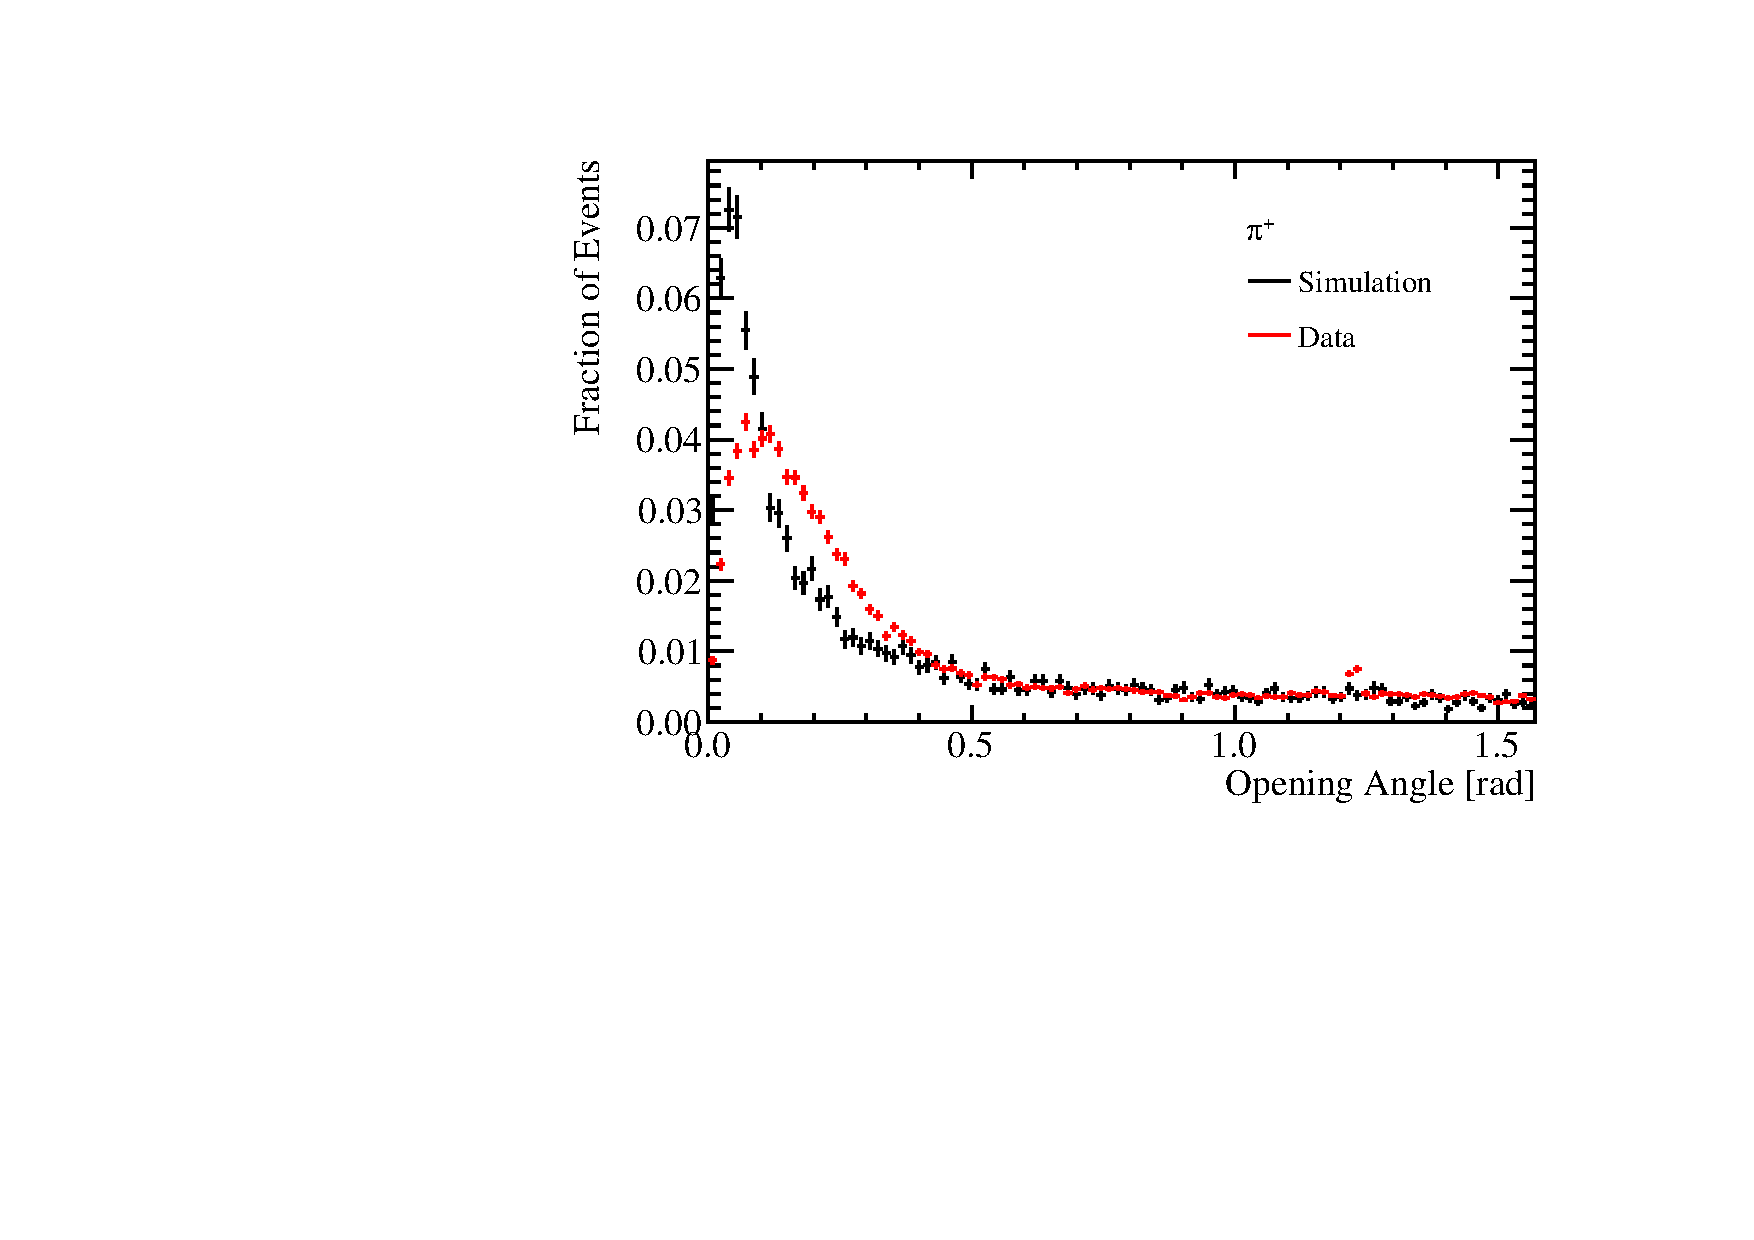
\includegraphics[width=0.5\textwidth]{Figures/Metrics/Data/Beam/BeamParticleOpeningAnglePiPlus.pdf}\label{fig:openingangletrk}}
\caption{\protect\subref{fig:openingangle} the opening angle between a linear fit to the start of the reconstructed test beam particle as it enters the TPC and the MC truth direction direction.  \protect\subref{fig:openingangleshw} and \protect\subref{fig:openingangletrk} show the same distributions for $e^{+}$ and $\pi^{+}$ triggered particles only.}
\label{fig:openingangles}
\end{figure}

\subsubsection{Cosmic-Ray Muon Reconstruction Metrics}

Reconstruction metrics for reconstructed cosmic-ray muon data have also been evaluated.  Figure \ref{fig:ncrdata} shows the number of reconstructed particles tagged as clear cosmic-ray muons per event in ProtoDUNE.  For a cosmic-ray muon to be tagged as clear it must deposit at least 100 hits in the detector.  This cut is applied in order to ensure a minimum reconstruction efficiency of ~90\%, based on the MC efficiencies in figure \ref{fig:crrecoeff}.  Therefore, this metric gives an accurate reflection of the true number of large cosmic-ray muons in the detector.  

There is excellent agreement between data and MC in the number of clear cosmic-ray muons per event, with both distributions peaking around 50 cosmic-ray muons per event.  The width of both distributions is similar, however the MC distribution is slightly broader and contains a high tail indicating that the MC flux is slightly overestimated in simulation.  

\begin{figure}
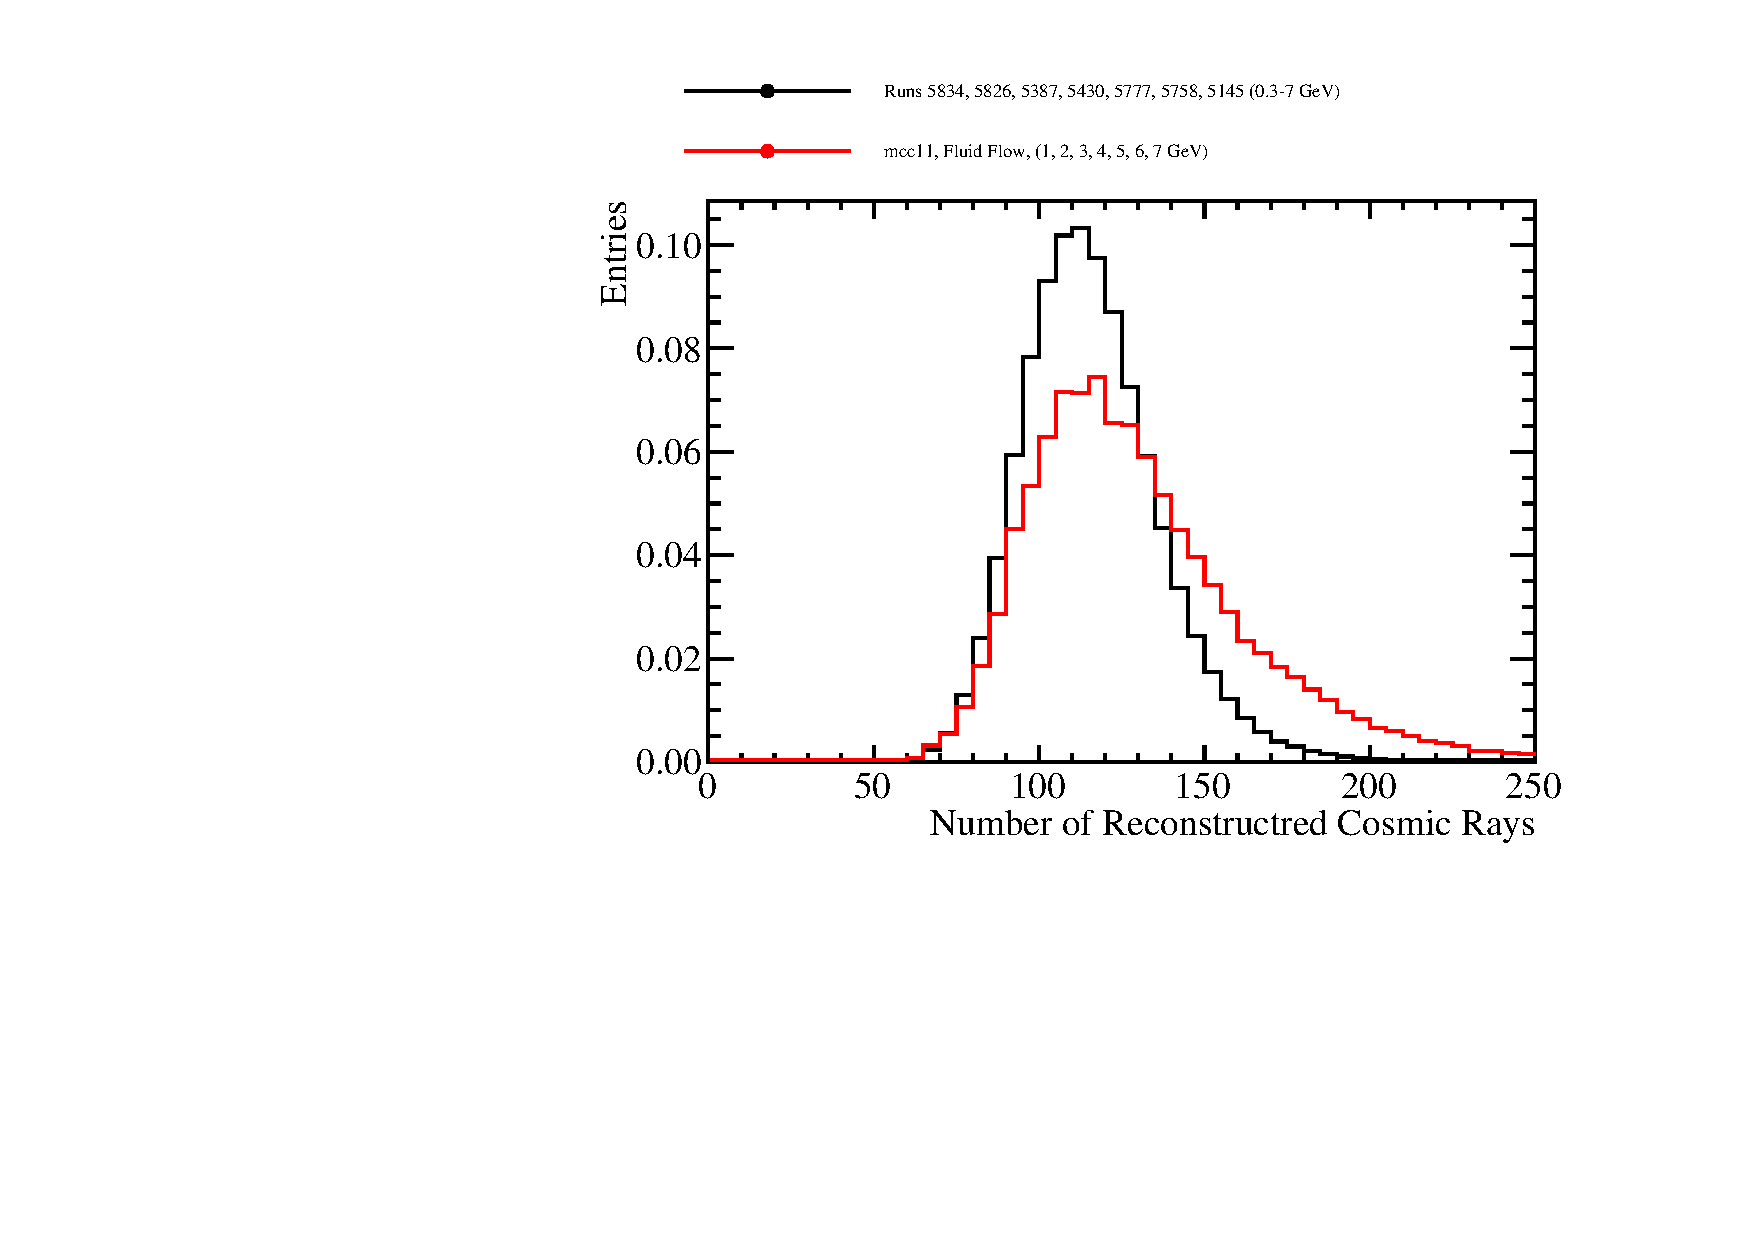
\includegraphics[width=1.0\textwidth]{Figures/Metrics/Data/Cosmics/NumberofReconstructedCosmicRays.pdf}
\caption{The number of reconstructed clear cosmic-ray muon particles per event.  A reconstructed particle is classified as a clear cosmic-ray muon if it has been reconstructed and tagged as a cosmic-ray muon and has deposited at least 100 hits in the detector.}
\label{fig:ncrdata}
\end{figure}

The distribution of the reconstructed $T_{0}$ values for cathode crossing cosmic-ray muons is shown in figure \ref{fig:recoT0data}.  The width of this distribution is determined by the readout time window and the drift time of the ProtoDUNE detector.  Both distributions for data and MC are in excellent agreement.  There height of the distribution is determined by the normalization of the plot.  There is a peak in the data reconstructed $T_{0}$ around 50~$\mu$s that is currently under investigation.  % Most likely due to CPA supports.

\begin{figure}
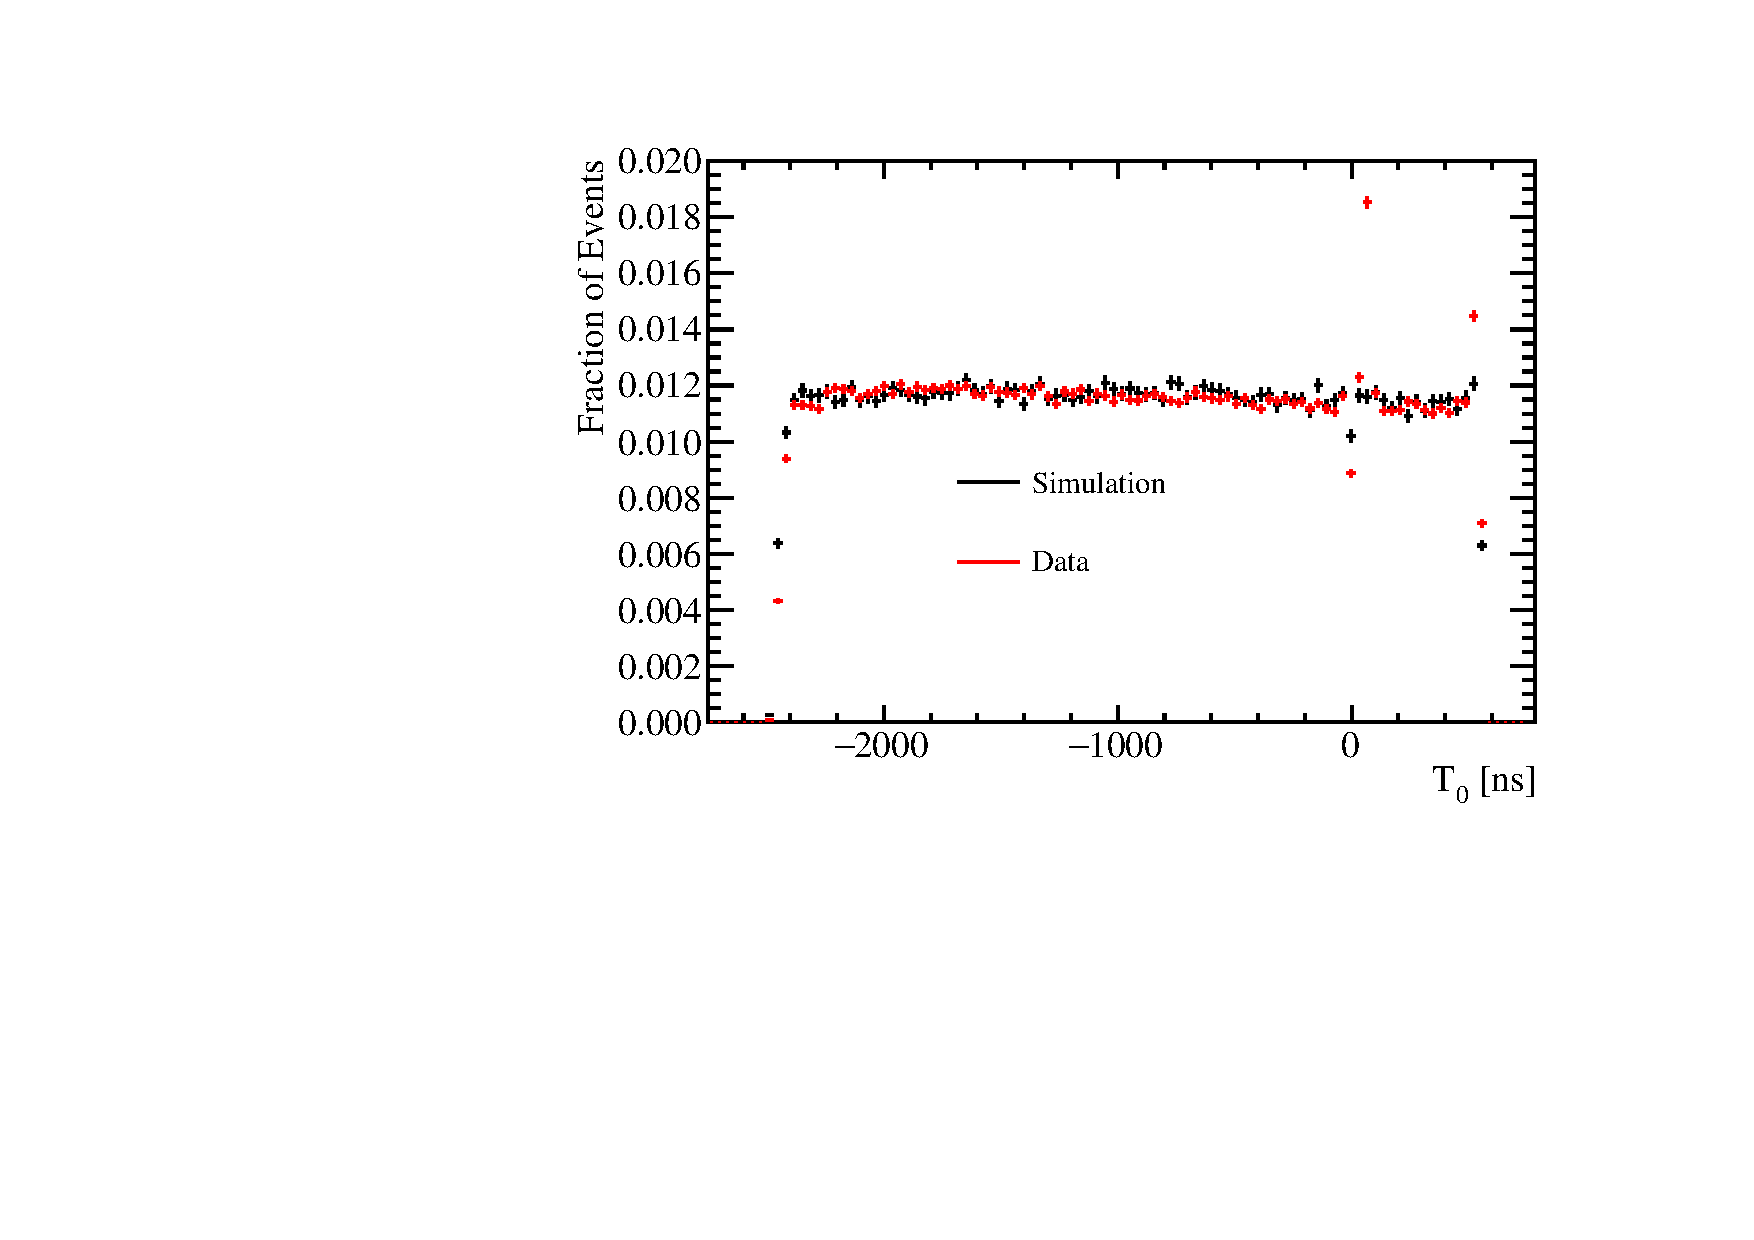
\includegraphics[width=1.0\textwidth]{Figures/Metrics/Data/Cosmics/StitchedT0.pdf}
\caption{The reconstructed $T_{0}$ distribution for data and MC.}
\label{fig:recoT0data}
\end{figure}

\section{Conclusions}
A summary of Pandora, a LArTPC pattern recognition software package, has been presented alongside relevant modifications allowing it to be applied to ProtoDUNE-SP.  The performance of Pandora has been extensively evaluated for simulation of the ProtoDUNE-SP detector.  Similarly, several pattern recognition metrics have been created and evaluated enabling a data MC comparison to be applied.  While differences are present, there is a generally good agreement between the two.  

The evaluation of the performance of Pandora for ProtoDUNE-SP is an important stepping stone in developing pattern recognition for the DUNE far detector.  The efficiencies quoted here must not be too readily extrapolated to the far detector.  Neutrino interactions in the far detector will be significantly easier to reconstruct in comparison to ProtoDUNE-SP because, unlike the underground far detector, ProtoDUNE-SP is a surface detector resulting in extensive cosmic-ray muon backgrounds.  The peak of the momentum distribution is  similar to what is expected from primary particles produced from neutrino interactions \todo{reference this}, therefore, the successful reconstruction of test beam particles is extremely encouraging for preparing a reconstruction for the DUNE far detector.  Additionally over the coming years developments to the pattern recognition are to be expected from the development of new algorithms and the incorporation of deep learning techniques.  

\begin{acknowledgements}
This material is based upon work supported by the following: The European Union’s Horizon 2020 Research and Innovation programme under grant agreement No. 776262.
\end{acknowledgements}

% BibTeX users please use one of
%\bibliographystyle{spbasic}      % basic style, author-year citations
%\bibliographystyle{spmpsci}      % mathematics and physical sciences
%\bibliographystyle{spphys}       % APS-like style for physics
%\bibliography{}   % name your BibTeX data base

% Non-BibTeX users please use
\begin{thebibliography}{}
%
% and use \bibitem to create references. Consult the Instructions
% for authors for reference list style.
%
\bibitem{pandorasdk}
Marshall, J. S. and Thomson, M. A., The Pandora Software Development Kit for Pattern Recognition, Eur. Phys. J., C75, 439 (2015)
\bibitem{pandorauboone}
Acciarri, R. and others, The Pandora multi-algorithm approach to automated pattern recognition of cosmic-ray muon and neutrino events in the MicroBooNE detector, Eur. Phys. J., C78, 82 (2018)
\bibitem{pdtdr}
Abi, B. and others [DUNE Collaboration], arXiv:1706.07081 [physics.ins-det]
%\bibitem{RefJ}
% Format for Journal Reference
%Author, Article title, Journal, Volume, page numbers (year)
% Format for books
%\bibitem{RefB}
%Author, Book title, page numbers. Publisher, place (year)
% etc
\end{thebibliography}

\end{document}
% end of file template.tex

